\documentclass[aspectratio=169, 10pt]{beamer}

% This is a template by Philipp Hennig for the University of Tuebingen.
% It was generated using ChatGPT by having it look in a similar style to the slides of Philipp Hennig.

% --- Packages ---
\usepackage{fontspec}
\usepackage{graphicx}
\usepackage{tikz}
\usetikzlibrary{shapes.geometric, positioning, arrows.meta}
\usepackage{xcolor}
\usepackage{amsmath, amssymb}
\usepackage{booktabs}
\usepackage{newunicodechar}
\usepackage{hyperref}
\usepackage{listings}
\usepackage[most]{tcolorbox} % Powerful box engine
\usepackage{eurosym} % Euro symbol support

% --- Bibliography ---
\usepackage[backend=biber, style=authoryear-comp, maxcitenames=2, maxbibnames=99, uniquename=false, uniquelist=false]{biblatex}
\addbibresource{references.bib}
% Smaller citation font for slides
\renewcommand*{\citesetup}{\tiny\color{TuebingenGray}}
\AtBeginBibliography{\tiny}

% --- Typography ---
\usefonttheme{professionalfonts}
\setmainfont{RobotoCondensed-Light}
\setsansfont{RobotoCondensed-Light}
\renewcommand{\familydefault}{\sfdefault}

% Map Unicode arrow to LaTeX command
\newunicodechar{→}{\ensuremath{\rightarrow}}

% --- COLOR PALETTE (Sampled from Screenshots) ---
\definecolor{TuebingenAnthrazit}{HTML}{32414B} % Dark Header/Text
\definecolor{TuebingenRot}{HTML}{A51E37}      % Primary Red
\definecolor{TuebingenGold}{HTML}{C5913E}      % Bullets / Strings
\definecolor{TuebingenGray}{HTML}{747D88}      % Footer
\definecolor{TuebingenGrayDark}{HTML}{5A6570} % Darker gray for theorem text
\definecolor{TuebingenGreen}{HTML}{4F8128}     % Code Border/Sidebar
\definecolor{TuebingenCyan}{HTML}{368CBF}      % Code methods (np.min)
\definecolor{TuebingenBeige}{HTML}{F5F6F6}     % Theorem Body Background

% --- Beamer Base Colors ---
\setbeamercolor{normal text}{fg=TuebingenAnthrazit}
\setbeamercolor{frametitle}{bg=TuebingenAnthrazit, fg=white}
\setbeamercolor{title}{fg=TuebingenRot}
\setbeamercolor{structure}{fg=TuebingenGold} 
\setbeamercolor{footline}{fg=TuebingenGray}

% --- Geometry ---
\setbeamersize{text margin left=0.8cm, text margin right=0.8cm}
\setbeamertemplate{navigation symbols}{}

% --- Bullets (Gold Triangles) ---
\setbeamertemplate{itemize item}{\scriptsize\raise1.25pt\hbox{\donotcoloroutermaths$\blacktriangleright$}}
\setbeamertemplate{itemize subitem}{\tiny\raise1.5pt\hbox{\donotcoloroutermaths$\blacktriangleright$}}

% --- METADATA ---
\newcommand{\lecturenumber}{01}
\newcommand{\coursename}{Strategic AI: From Vision to Value}
\newcommand{\license}{CC BY-SA 4.0}
\newcommand{\shortdate}{07/01/2026}
\newcommand{\longdate}{7 January 2026}
\title{AI and Coding for C-Level Executives: Foundations, Methods, and Business Patterns}
\subtitle{Guinea Pigs: Jan Köberle and Gabriel Käppler}
\author{Niklas Abraham}

% Faculty/Department/Chair for title slide (see template usage)
\newcommand{\facultyname}{Faculty of Science}
\newcommand{\departmentname}{Department of Computer Science}
\newcommand{\chairname}{Chair of Artificial Intelligence}

% --- SOURCE PLACEHOLDER ---
% Use \framesource{Your source text} in a frame to set the source
\makeatletter
\newcommand{\framesource}[1]{\gdef\@framesource{#1}}
\framesource{} % Initialize as empty

% --- BACKGROUND IMAGE FOR TITLE PAGE ---
% Use \titlebgimage{filename.jpg} to set a background image for the title page
\newcommand{\titlebgimage}[1]{\gdef\@titlebgimage{#1}}
\titlebgimage{} % Initialize as empty
\makeatother

% ==============================================================================
%   SPECIAL ELEMENTS
% ==============================================================================

% 1. THEOREM BOX (Red Header, Beige Body)
% Matches: image_fcac79.png
\newtcolorbox{theorembox}[2][]{
    enhanced,
    colback=TuebingenBeige,      % Light beige interior
    colframe=TuebingenRot,       % Red border
    colbacktitle=TuebingenRot,   % Red Title background
    coltitle=white,              % White Title text
    coltext=TuebingenAnthrazit,  % Dark grey text color (#32414b)
    fonttitle=\bfseries\large,
    title={#2},
    arc=4pt, outer arc=4pt,      % Rounded corners
    boxrule=0.8pt,               % Thin border
    left=6pt, right=6pt, top=6pt, bottom=6pt,
    titlerule=0mm,
    toptitle=0.8mm, bottomtitle=0.8mm,  % Slimmer red title bar
    width=0.95\textwidth,        % Make theorem block narrower
    center,                      % Center the narrower box
    #1
}

% 2. CODE BOX (Green Border, Green Sidebar)
% Matches: image_fcac1f.png
\newtcolorbox{codebox}{
    enhanced,
    colback=white,
    colframe=TuebingenGreen,     % Green Border
    arc=5pt, outer arc=5pt,      % Rounded corners on all sides
    boxrule=1.5pt,               % Thicker border
    left=6mm,                    % Space for sidebar
    top=0mm, bottom=0mm,
    overlay={
        % The Solid Green Sidebar for numbers with rounded left corners
        \fill[TuebingenGreen, rounded corners=5pt] 
            (frame.south west) -- 
            ([xshift=6mm]frame.south west) -- 
            ([xshift=6mm]frame.north west) -- 
            (frame.north west) -- 
            cycle;
    }
}

% 3. CODE LISTING STYLE
\lstdefinestyle{TuebingenStyle}{
    language=Python,
    basicstyle=\ttfamily\footnotesize\color{black},
    keywordstyle=\color{TuebingenRot}\bfseries, % import, as
    stringstyle=\color{TuebingenGold},          % "strings"
    commentstyle=\color{TuebingenGreen},        % # comments
    identifierstyle=\color{black},
    % Custom highlighting for methods like .min
    classoffset=1, 
    morekeywords={min, max, mean, array, choice},
    keywordstyle=\color{TuebingenCyan}, 
    classoffset=0,
    numbers=left,
    numberstyle=\scriptsize\color{white}\hfill,   % Line number centered in its space
    numbersep=10pt,
    breaklines=true,
    showstringspaces=false,
    frame=none
}
\lstset{style=TuebingenStyle}

% Python style for code comparison
\lstdefinestyle{pythonstyle}{
    language=Python,
    basicstyle=\ttfamily\tiny\color{black},
    keywordstyle=\color{TuebingenRot}\bfseries,
    stringstyle=\color{TuebingenGold},
    commentstyle=\color{TuebingenGreen}\itshape,
    numbers=left,
    numberstyle=\tiny\color{white}\hfill,
    numbersep=8pt,
    breaklines=true,
    showstringspaces=false,
    frame=none,
    morekeywords={as, with, True, False, None}
}

% Java style for code comparison
\lstdefinestyle{javastyle}{
    language=Java,
    basicstyle=\ttfamily\tiny\color{black},
    keywordstyle=\color{TuebingenRot}\bfseries,
    stringstyle=\color{TuebingenGold},
    commentstyle=\color{TuebingenGreen}\itshape,
    numbers=left,
    numberstyle=\tiny\color{white}\hfill,
    numbersep=8pt,
    breaklines=true,
    showstringspaces=false,
    frame=none,
    morekeywords={var, record}
}

% Go style for code comparison
\lstdefinestyle{gostyle}{
    language=C,
    basicstyle=\ttfamily\tiny\color{black},
    keywordstyle=\color{TuebingenRot}\bfseries,
    stringstyle=\color{TuebingenGold},
    commentstyle=\color{TuebingenGreen}\itshape,
    numbers=left,
    numberstyle=\tiny\color{white}\hfill,
    numbersep=8pt,
    breaklines=true,
    showstringspaces=false,
    frame=none,
    morekeywords={func, defer, range, nil, error, fmt, os, float64, int}
}

% ==============================================================================
%   SLIDE LAYOUTS
% ==============================================================================

% --- HEADER (Dark Bar + Logo) ---
\makeatletter
\setbeamertemplate{frametitle}{
    \nointerlineskip
    \begin{beamercolorbox}[wd=\paperwidth, ht=1.2cm, dp=0.3cm]{frametitle}
        \begin{tikzpicture}
            \useasboundingbox (0,0) rectangle (\paperwidth,1.2);
            % Title
            \node[anchor=north west, white, align=left] at (0.25, 1.05) {\Large \insertframetitle};
            % Subtitle
            \node[anchor=north west, color=gray!50, align=left] at (0.25, 0.3) {\small \insertframesubtitle};
            % Logo (Top Right)
            \node[anchor=north east] at (\paperwidth-0.2cm, 1.1) {
                \IfFileExists{logo_white.png}{
                    \includegraphics[height=0.665cm]{logo_white.png}
                }{
                    \tikz\node[draw=white, text=white, inner sep=2pt] {\scriptsize LOGO};
                }
            };
            % Sources Placeholder (Below Logo)
            \node[anchor=north east, align=right] at (\paperwidth-0.2cm, 0.25) {
                \small \color{gray!50} 
                \ifx\@framesource\empty
                    % then empty
                    \textcolor{white}{ }
                \else
                    \@framesource
                \fi
            };
        \end{tikzpicture}
    \end{beamercolorbox}
}
\makeatother

% --- FOOTER (Standard) ---
\setbeamertemplate{footline}{
    \ifnum\thepage>1 % Skip footer on title page (usually)
    \begin{tikzpicture}[remember picture, overlay]
        \node[anchor=south west, align=left] at ([xshift=0.5cm, yshift=0.2cm]current page.south west) {
            \tiny \color{TuebingenGray} Course Name \#\lecturenumber \ -- \ \the\year \ \insertauthor, \license \ -- \ \shortdate
        };
        \node[anchor=south east, align=right] at ([xshift=-0.5cm, yshift=0.2cm]current page.south east) {
            \tiny \color{TuebingenGray} \insertframenumber
        };
    \end{tikzpicture}
    \fi
}

% --- TITLE PAGE (Complex Layout) ---
\makeatletter
\setbeamertemplate{title page}{
    \begin{tikzpicture}[remember picture, overlay]
        % Optional Background Image
        \ifx\@titlebgimage\empty
            % No background image, use white background
        \else
            \node[anchor=center, opacity=0.15] at (current page.center) {
                \includegraphics[width=\paperwidth, height=\paperheight, keepaspectratio=false]{\@titlebgimage}
            };
        \fi
        
        % 1. Titles (Top Center) - Smaller now
        \node[anchor=north, align=center] at ([yshift=-1.5cm]current page.north) {
            {\LARGE \color{TuebingenRot} \textsc{\coursename}} \\[0.15cm]
            {\normalsize \color{TuebingenAnthrazit} \textsc{\inserttitle}} \\[0.05cm]
            {\small \color{TuebingenAnthrazit} \textsc{\insertsubtitle}}
        };

        % 2. Author and Date (Center)
        \node[anchor=center, align=center] at ([yshift=0.3cm]current page.center) {
            {\large \insertauthor} \\[0.3cm]
            {\normalsize \longdate}
        };

        % 3. Logos (Lower Third)
        \node[anchor=south, align=center] at ([yshift=1cm, xshift=0.5cm]current page.south) {
            \begin{minipage}{0.9\textwidth}
                \centering
                % Left: Logo
                \begin{minipage}{0.35\textwidth}
                    \raggedright
                    \IfFileExists{logo_red.png}{
                        \includegraphics[height=2cm]{logo_red.png}
                    }{
                        % Fallback if logo doesn't exist
                    }
                \end{minipage}%
            \end{minipage}
        };

    \end{tikzpicture}
}
\makeatother

% ==============================================================================
%   CONTENT
% ==============================================================================

\begin{document}


% --- 1. TITLE SLIDE ---
\begin{frame}[plain]
    \titlepage
\end{frame}

% --- 2. OUTLINE SLIDE ---
\begin{frame}{Today's Agenda}
    \framesubtitle{What we will cover in this executive briefing}
    \begin{itemize}
        \item \textbf{Act 0: Software Literacy Primer}\\
        \ \small Programming languages, editors, databases, compute
        \item \textbf{Act I: AI Foundations and History}\\
        \ \small What AI is, why now, and the timeline
        \item \textbf{Act II: Modern AI Methods (Deep Dive)}\\
        \ \small From classical ML to deep learning, transformers, RAG, evaluation
        \item \textbf{Act III: Business Patterns}\\
        \ \small Repeatable templates for AI in business
        \item \textbf{Act IV: Governance and Economics}\\
        \ \small Operating models, benchmarking, cost, vendor strategy
        \item \textbf{Act V: Transition and Q\&A}\\
        \ \small Tailored analysis and open questions
    \end{itemize}
    \vspace{0.5em}
    {\small\color{TuebingenGray} Breaks and deep-dive sessions are scheduled throughout.}
\end{frame}

% ==============================================================================
%   INCLUDE ACT CHAPTERS
% ==============================================================================

% Act 0 — Software Literacy Primer
\section{Orientation: Software Foundations Executives Need}

% ==============================================================================
% 0.1 The "Stack Map" (1 slide)
% ==============================================================================

\begin{frame}{The Technology Stack: AI in Context}
    \framesubtitle{Understanding where AI fits in your organization}
    
    {\color{TuebingenGray} AI is not magic—it's software built on data, running on infrastructure, serving business processes.}
    
    \vspace{0.8em}
    \begin{center}
        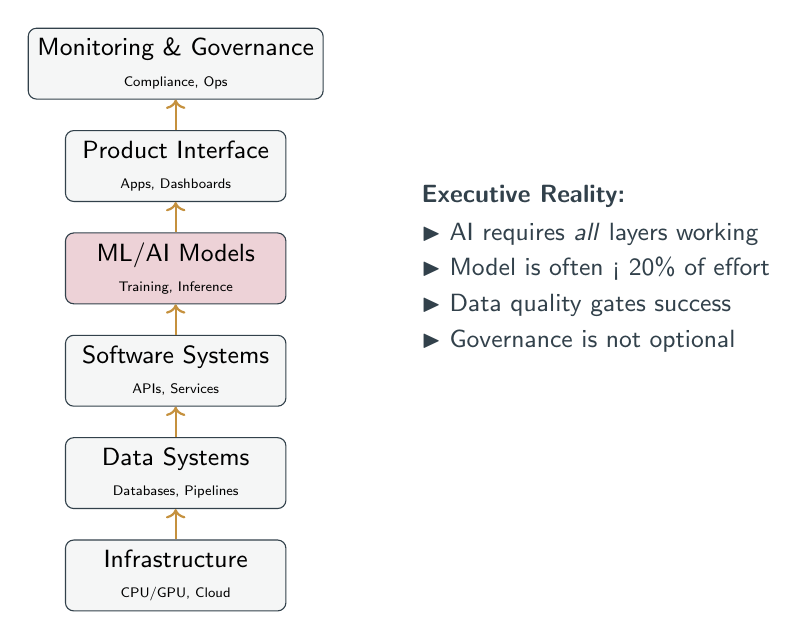
\begin{tikzpicture}[
            box/.style={draw=TuebingenAnthrazit, rounded corners=3pt, minimum width=2.8cm, minimum height=0.9cm, align=center, font=\small},
            arrow/.style={->, thick, TuebingenGold}
        ]
            % Stack layers (bottom to top)
            \node[box, fill=TuebingenBeige] (infra) at (0,0) {Infrastructure\\{\tiny CPU/GPU, Cloud}};
            \node[box, fill=TuebingenBeige] (data) at (0,1.3) {Data Systems\\{\tiny Databases, Pipelines}};
            \node[box, fill=TuebingenBeige] (software) at (0,2.6) {Software Systems\\{\tiny APIs, Services}};
            \node[box, fill=TuebingenRot!20] (ai) at (0,3.9) {ML/AI Models\\{\tiny Training, Inference}};
            \node[box, fill=TuebingenBeige] (product) at (0,5.2) {Product Interface\\{\tiny Apps, Dashboards}};
            \node[box, fill=TuebingenBeige] (govern) at (0,6.5) {Monitoring \& Governance\\{\tiny Compliance, Ops}};
            
            % Arrows
            \draw[arrow] (infra) -- (data);
            \draw[arrow] (data) -- (software);
            \draw[arrow] (software) -- (ai);
            \draw[arrow] (ai) -- (product);
            \draw[arrow] (product) -- (govern);
            
            % Business context
            \node[anchor=west, align=left, font=\small, TuebingenAnthrazit] at (3,3.9) {
                \textbf{Executive Reality:}\\[0.3em]
                $\blacktriangleright$ AI requires \textit{all} layers working\\[0.2em]
                $\blacktriangleright$ Model is often < 20\% of effort\\[0.2em]
                $\blacktriangleright$ Data quality gates success\\[0.2em]
                $\blacktriangleright$ Governance is not optional
            };
        \end{tikzpicture}
    \end{center}
    
    \vspace{0.5em}
    \begin{center}
        \small\color{TuebingenRot} \textbf{Key insight:} "AI" is software + data + evaluation. Invest across the stack.
    \end{center}
\end{frame}

% ==============================================================================
% 0.2 Programming Languages: What Exists and Why It Matters (2 slides)
% ==============================================================================

\begin{frame}{Programming Languages: The Landscape}
    \framesubtitle{Why language choice matters for your AI initiatives}
    
    {\color{TuebingenGray} Different languages serve different purposes. Understanding this helps evaluate team composition and vendor choices.}
    
    \vspace{0.5em}
    \begin{columns}[T]
        \column{0.48\textwidth}
        \textbf{\color{TuebingenRot}Data \& ML Ecosystem:}
        \begin{itemize}
            \setlength\itemsep{0.3em}
            \item \textbf{Python} — dominant for ML/AI
                \begin{itemize}
                    \item Rich libraries (TensorFlow, PyTorch)
                    \item Rapid prototyping
                    \item Data science standard
                \end{itemize}
            \item \textbf{R / MATLAB} — statistical analysis niches
        \end{itemize}
        
        \vspace{0.5em}
        \textbf{\color{TuebingenGold}Enterprise \& Backend:}
        \begin{itemize}
            \setlength\itemsep{0.3em}
            \item \textbf{Java} — enterprise systems, stability
            \item \textbf{Go} — cloud infrastructure, concurrency
            \item \textbf{C\#} — Microsoft ecosystem
        \end{itemize}
        
        \column{0.48\textwidth}
        \textbf{\color{TuebingenGreen}Performance-Critical:}
        \begin{itemize}
            \setlength\itemsep{0.3em}
            \item \textbf{C/C++} — model runtimes, systems
            \item \textbf{Rust} — safety + performance
            \item \textbf{CUDA} — GPU programming
        \end{itemize}
        
        \vspace{0.5em}
        \textbf{\color{TuebingenCyan}Product Interfaces:}
        \begin{itemize}
            \setlength\itemsep{0.3em}
            \item \textbf{JavaScript/TypeScript} — web, full-stack
            \item \textbf{Swift/Kotlin} — mobile apps
        \end{itemize}
        
        \vspace{0.5em}
        \textbf{\color{TuebingenAnthrazit}Specialized:}
        \begin{itemize}
            \setlength\itemsep{0.3em}
            \item \textbf{Haskell/Scala} — type safety, correctness
            \item \textbf{SQL} — data querying (ubiquitous)
        \end{itemize}
    \end{columns}
\end{frame}

\begin{frame}{Why Language Choice Matters for AI}
    \framesubtitle{Ecosystems, talent, and AI assistance quality}
    
    \vspace{0.5em}
    \begin{columns}[T]
        \column{0.55\textwidth}
        \textbf{The "Gravity Well" Effect:}
        \begin{itemize}
            \setlength\itemsep{0.5em}
            \item ML research concentrates in \textbf{Python}
            \item Enterprise gravity in \textbf{Java/Go}
            \item Performance work in \textbf{C++/Rust}
            \item Each ecosystem has its own:
                \begin{itemize}
                    \item Package libraries
                    \item Community expertise
                    \item Hiring pool
                \end{itemize}
        \end{itemize}
        
        \column{0.42\textwidth}
        \begin{theorembox}{AI Coding Assistant Quality}
            LLM coding tools perform best where \textbf{training data is abundant}.
            
            \vspace{0.3em}
            {\small
            \textbf{Strong support:} Python, JavaScript, Java, Go
            
            \textbf{Moderate:} C++, Rust, TypeScript
            
            \textbf{Weaker:} MATLAB, R, niche languages}
        \end{theorembox}
    \end{columns}
    
    \vspace{0.8em}
    \begin{center}
        \small\color{TuebingenRot} \textbf{Executive takeaway:} Language choice shapes experimentation speed, maintainability, hiring, and AI-assistance leverage.
    \end{center}
\end{frame}

% ==============================================================================
% 0.3 One Identical Example in Three Languages (3 slides)
% ==============================================================================

\begin{frame}[fragile]{Code Comparison: The Same Task in Three Languages}
    \framesubtitle{Task: Load CSV, compute summary, detect anomalies, output JSON}
    
    {\color{TuebingenGray} Seeing the same logic expressed differently reveals language philosophies.}
    
    \vspace{0.5em}
    \begin{columns}[T]
        \column{0.48\textwidth}
        \begin{codebox}
            {\small\textbf{\color{TuebingenGreen}Python} — Concise, library-rich}
            \vspace{0.3em}
\begin{lstlisting}[style=pythonstyle, basicstyle=\ttfamily\tiny]
import pandas as pd
import json

# Load and analyze
df = pd.read_csv("transactions.csv")
summary = {
    "total": df["amount"].sum(),
    "mean": df["amount"].mean(),
    "count": len(df)
}

# Detect anomalies (simple rule)
threshold = summary["mean"] * 3
anomalies = df[df["amount"] > threshold]
summary["anomalies"] = len(anomalies)

# Output
with open("report.json", "w") as f:
    json.dump(summary, f)
\end{lstlisting}
        \end{codebox}
        
        \column{0.48\textwidth}
        {\small\color{TuebingenAnthrazit}
        \textbf{Characteristics:}
        \begin{itemize}
            \setlength\itemsep{0.2em}
            \item 15 lines of code
            \item Rich standard library
            \item Readable, minimal boilerplate
            \item Dynamic typing (flexible)
            \item Dominant in data science
        \end{itemize}
        
        \vspace{0.5em}
        \textbf{Trade-offs:}
        \begin{itemize}
            \setlength\itemsep{0.2em}
            \item Slower runtime than compiled
            \item Type errors found at runtime
            \item GIL limits parallelism
        \end{itemize}
        }
    \end{columns}
\end{frame}

\begin{frame}[fragile]{Code Comparison: Java — Enterprise Standard}
    \framesubtitle{Same task: More structure, explicit types, verbose}
    
    \begin{columns}[T]
        \column{0.55\textwidth}
        \begin{codebox}
            {\small\textbf{\color{TuebingenGreen}Java} — Explicit, structured}
            \vspace{0.2em}
\begin{lstlisting}[style=javastyle, basicstyle=\ttfamily\tiny]
public class TransactionAnalyzer {
    public static void main(String[] args) {
        List<Transaction> txns = loadCSV("transactions.csv");
        
        double total = txns.stream()
            .mapToDouble(Transaction::getAmount)
            .sum();
        double mean = total / txns.size();
        double threshold = mean * 3;
        
        long anomalyCount = txns.stream()
            .filter(t -> t.getAmount() > threshold)
            .count();
        
        Summary summary = new Summary(
            total, mean, txns.size(), anomalyCount);
        
        ObjectMapper mapper = new ObjectMapper();
        mapper.writeValue(
            new File("report.json"), summary);
    }
}
\end{lstlisting}
        \end{codebox}
        
        \column{0.42\textwidth}
        {\small\color{TuebingenAnthrazit}
        \textbf{Characteristics:}
        \begin{itemize}
            \setlength\itemsep{0.2em}
            \item ~25 lines (plus class definitions)
            \item Static typing (compile-time safety)
            \item Explicit structure
            \item Enterprise conventions
            \item Long-lived, maintainable codebases
        \end{itemize}
        
        \vspace{0.5em}
        \textbf{Trade-offs:}
        \begin{itemize}
            \setlength\itemsep{0.2em}
            \item More boilerplate
            \item Slower iteration
            \item Steeper learning curve
        \end{itemize}
        }
    \end{columns}
\end{frame}

\begin{frame}[fragile]{Code Comparison: Go — Modern Systems Language}
    \framesubtitle{Same task: Explicit error handling, built for services}
    
    \begin{columns}[T]
        \column{0.55\textwidth}
        \begin{codebox}
            {\small\textbf{\color{TuebingenGreen}Go} — Explicit, concurrent-ready}
            \vspace{0.2em}
\begin{lstlisting}[style=gostyle, basicstyle=\ttfamily\tiny]
func analyzeTransactions() error {
    file, err := os.Open("transactions.csv")
    if err != nil {
        return fmt.Errorf("open: %w", err)
    }
    defer file.Close()
    
    txns, err := parseCSV(file)
    if err != nil {
        return fmt.Errorf("parse: %w", err)
    }
    
    var total float64
    for _, t := range txns {
        total += t.Amount
    }
    mean := total / float64(len(txns))
    threshold := mean * 3
    
    var anomalies int
    for _, t := range txns {
        if t.Amount > threshold {
            anomalies++
        }
    }
    
    summary := Summary{Total: total, Mean: mean,
        Count: len(txns), Anomalies: anomalies}
    return writeJSON("report.json", summary)
}
\end{lstlisting}
        \end{codebox}
        
        \column{0.42\textwidth}
        {\small\color{TuebingenAnthrazit}
        \textbf{Characteristics:}
        \begin{itemize}
            \setlength\itemsep{0.2em}
            \item ~30 lines
            \item \textbf{Explicit error handling}
            \item Compiled, fast execution
            \item Built-in concurrency
            \item Cloud/DevOps standard
        \end{itemize}
        
        \vspace{0.5em}
        \textbf{Go Philosophy:}
        \begin{itemize}
            \setlength\itemsep{0.2em}
            \item "Errors are values"
            \item Simplicity over cleverness
            \item Designed for services
        \end{itemize}
        
        \vspace{0.5em}
        \color{TuebingenRot}\small\textit{Used by: Docker, Kubernetes, most cloud infrastructure}
        }
    \end{columns}
\end{frame}

% ==============================================================================
% 0.5 Editors and AI Coding Copilots (1 slide)

% ------------------------------------------------------------------------------
\begin{frame}{Development Tools: Editors and AI Coding Assistants}
    \framesubtitle{The delivery vehicle for AI in engineering}
    {\color{TuebingenGray} Modern editors are where AI meets developers—and where governance matters most.}
    \vspace{0.5em}
    \begin{columns}[T]
        \column{0.48\textwidth}
        	extbf{Popular Development Environments:}
        \begin{itemize}
            \setlength\itemsep{0.4em}
            \item \textbf{VS Code}: Free, open source, huge extension ecosystem, strong AI integration (Copilot, etc.), cross-platform. Used by individuals and enterprises.
            \item \textbf{Cursor}: AI-native fork of VS Code, built-in copilots, context window navigation, paid plans for advanced AI features.
            \item \textbf{JetBrains Suite} (IntelliJ, PyCharm, etc.): Paid, advanced refactoring, deep language support, enterprise features, strong static analysis, AI assistant (paid add-on).
            \item \textbf{Vim/Neovim}: Free, highly customizable, keyboard-driven, used on servers and by power users. AI plugins available.
        \end{itemize}
        \vspace{0.5em}
        	extbf{AI Coding Assistant Capabilities:}
        \begin{itemize}
            \setlength\itemsep{0.3em}
            \item Code completion (line/block)
            \item Refactoring suggestions
            \item Test generation
            \item Documentation writing
            \item Code search and explanation
            \item Agentic workflows (bounded)
        \end{itemize}
        \column{0.48\textwidth}
        \begin{theorembox}{Governance Implications}
            AI coding tools require explicit policies:
            \vspace{0.3em}
            \begin{itemize}
                \setlength\itemsep{0.3em}
                \item \textbf{Secrets} — API keys, credentials exposure
                \item \textbf{IP/Licensing} — training data, code ownership
                \item \textbf{Security} — vulnerable code suggestions
                \item \textbf{Auditability} — who wrote what?
                \item \textbf{Data residency} — where does code go?
            \end{itemize}
        \end{theorembox}
        \vspace{0.3em}
        {\small\color{TuebingenRot} \textit{Productivity gains of 20-40\% reported, but governance is non-negotiable.}}
    \end{columns}
\end{frame}

\begin{frame}{Editor Comparison: Features and Pricing}
    \framesubtitle{What do you get, and at what cost?}
    \begin{center}
    \begin{tabular}{|l|l|l|l|}
        \hline
        	extbf{Editor} & \textbf{Key Features} & \textbf{AI Integration} & \textbf{Pricing} \\
        \hline
        VS Code & Extensible, cross-platform & Copilot, 3rd-party & Free \\
        Cursor & AI-native, context tools & Built-in, advanced & Free basic, Paid Pro (\euro20+/mo) \\
        JetBrains & Refactoring, static analysis & AI Assistant (add-on) & \euro20-50/mo/user \\
        Vim/Neovim & Lightweight, scriptable & Plugins (Copilot, etc.) & Free \\
        \hline
    \end{tabular}
    \end{center}
    \vspace{0.5em}
    {\small\color{TuebingenGray} *Prices as of 2026, may vary by region and plan.}
\end{frame}

% ==============================================================================
% 0.6 Database Systems Overview (2 slides)
% ==============================================================================

\begin{frame}{Database Systems: Choosing the Right Tool}
    \framesubtitle{Different data patterns require different systems}
    
    {\color{TuebingenGray} "Which database?" is really "What are your query patterns and constraints?"}
    
    \vspace{0.3em}
    \begin{columns}[T]
        \column{0.48\textwidth}
        \textbf{\color{TuebingenRot}Relational (SQL):}
        \begin{itemize}
            \setlength\itemsep{0.2em}
            \item PostgreSQL, MySQL, Oracle
            \item Transactions, consistency, reporting
            \item Structured business data
            \item \textit{Most enterprise use cases}
        \end{itemize}
        
        \vspace{0.3em}
        \textbf{\color{TuebingenGold}Document Stores:}
        \begin{itemize}
            \setlength\itemsep{0.2em}
            \item MongoDB, CouchDB
            \item Flexible schemas
            \item Product data, events, logs
        \end{itemize}
        
        \vspace{0.3em}
        \textbf{\color{TuebingenGreen}Key-Value Stores:}
        \begin{itemize}
            \setlength\itemsep{0.2em}
            \item Redis, DynamoDB
            \item Caching, session state
            \item Sub-millisecond latency
        \end{itemize}
        
        \column{0.48\textwidth}
        \textbf{\color{TuebingenCyan}Columnar / Data Warehouses:}
        \begin{itemize}
            \setlength\itemsep{0.2em}
            \item Snowflake, BigQuery, Redshift
            \item Analytics at scale
            \item Historical analysis, BI
        \end{itemize}
        
        \vspace{0.3em}
        \textbf{\color{TuebingenAnthrazit}Graph Databases:}
        \begin{itemize}
            \setlength\itemsep{0.2em}
            \item Neo4j, Amazon Neptune
            \item Relationships, knowledge graphs
            \item Entity resolution, networks
        \end{itemize}
        
        \vspace{0.3em}
        \textbf{\color{TuebingenRot}Vector Databases:}
        \begin{itemize}
            \setlength\itemsep{0.2em}
            \item Pinecone, Weaviate, Qdrant
            \item \textbf{Embeddings for RAG/AI}
            \item Similarity search
        \end{itemize}
    \end{columns}
\end{frame}

\begin{frame}{Database Selection: Executive Decision Framework}
    \framesubtitle{Match the system to your constraints}
    
    \vspace{0.5em}
    \begin{center}
        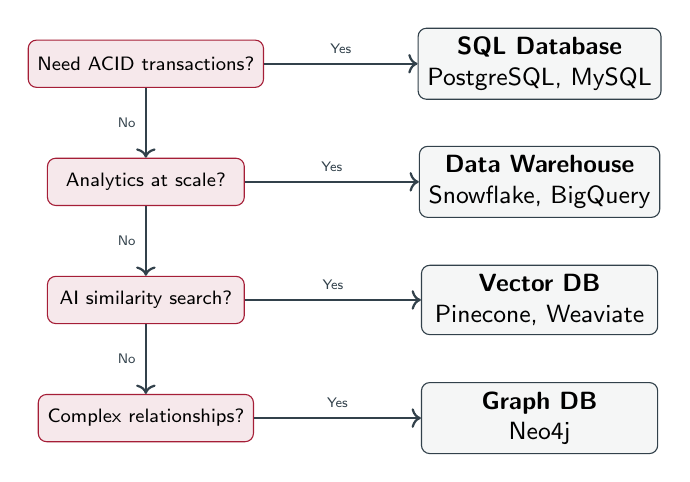
\begin{tikzpicture}[
            node distance=1.5cm,
            box/.style={draw=TuebingenAnthrazit, rounded corners=3pt, minimum width=3cm, minimum height=0.8cm, align=center, font=\small, fill=TuebingenBeige},
            decision/.style={draw=TuebingenRot, rounded corners=3pt, minimum width=2.5cm, minimum height=0.6cm, align=center, font=\scriptsize, fill=TuebingenRot!10},
            arrow/.style={->, thick, TuebingenAnthrazit}
        ]
            \node[decision] (q1) at (0,0) {Need ACID transactions?};
            \node[box] (sql) at (5,0) {\textbf{SQL Database}\\PostgreSQL, MySQL};
            \node[decision] (q2) at (0,-1.5) {Analytics at scale?};
            \node[box] (warehouse) at (5,-1.5) {\textbf{Data Warehouse}\\Snowflake, BigQuery};
            \node[decision] (q3) at (0,-3) {AI similarity search?};
            \node[box] (vector) at (5,-3) {\textbf{Vector DB}\\Pinecone, Weaviate};
            \node[decision] (q4) at (0,-4.5) {Complex relationships?};
            \node[box] (graph) at (5,-4.5) {\textbf{Graph DB}\\Neo4j};
            
            \draw[arrow] (q1) -- node[above]{\tiny Yes} (sql);
            \draw[arrow] (q1) -- node[left]{\tiny No} (q2);
            \draw[arrow] (q2) -- node[above]{\tiny Yes} (warehouse);
            \draw[arrow] (q2) -- node[left]{\tiny No} (q3);
            \draw[arrow] (q3) -- node[above]{\tiny Yes} (vector);
            \draw[arrow] (q3) -- node[left]{\tiny No} (q4);
            \draw[arrow] (q4) -- node[above]{\tiny Yes} (graph);
        \end{tikzpicture}
    \end{center}
    
    \vspace{0.5em}
    \begin{theorembox}{Executive Rule of Thumb}
        Choose databases based on \textbf{query patterns} and \textbf{constraints} (latency, consistency, scale)—not vendor marketing or "fashion". Most organizations need \textbf{multiple} database types working together.
    \end{theorembox}
\end{frame}

% ==============================================================================
% 0.7 Compute Basics: CPU vs GPU (1 slide)

% ------------------------------------------------------------------------------
\begin{frame}{Compute Infrastructure: CPU, GPU, and Beyond}
    \framesubtitle{Understanding what powers AI workloads}
    {\color{TuebingenGray} AI's compute demands are fundamentally different from traditional software.}
    \vspace{0.5em}
    \begin{columns}[T]
        \column{0.32\textwidth}
        \begin{center}
            {\Large \color{TuebingenRot} \textbf{CPU}}
        \end{center}
        \vspace{0.2em}
        \begin{itemize}
            \setlength\itemsep{0.2em}
            \item General-purpose processor for all software
            \item Handles complex logic, branching, and orchestration
            \item Low to moderate parallelism (8-64 cores typical)
            \item Used for data processing, serving, business logic
            \item Widely available, cost-effective
        \end{itemize}
        \vspace{0.3em}
        {\scriptsize\color{TuebingenGray} \textit{Best for: Traditional software, ETL, web servers, orchestration}}
        \column{0.32\textwidth}
        \begin{center}
            {\Large \color{TuebingenGold} \textbf{GPU}}
        \end{center}
        \vspace{0.2em}
        \begin{itemize}
            \setlength\itemsep{0.2em}
            \item Massively parallel (10,000+ cores)
            \item Optimized for matrix math, deep learning
            \item Essential for AI model training and fast inference
            \item High memory bandwidth, but expensive
            \item Used in cloud and on-prem for ML/AI
        \end{itemize}
        \vspace{0.3em}
        {\scriptsize\color{TuebingenGray} \textit{Best for: Deep learning, large-scale analytics, simulation}}
        \column{0.32\textwidth}
        \begin{center}
            {\Large \color{TuebingenGreen} \textbf{TPU/NPU}}
        \end{center}
        \vspace{0.2em}
        \begin{itemize}
            \setlength\itemsep{0.2em}
            \item AI-specialized silicon (Google TPU, Apple NPU, etc.)
            \item Even more efficient for neural nets
            \item Used in cloud (TPU) and edge/mobile (NPU)
            \item Vendor lock-in risk, less flexible
            \item Can dramatically reduce inference cost at scale
        \end{itemize}
        \vspace{0.3em}
        {\scriptsize\color{TuebingenGray} \textit{Best for: Cloud AI services, edge inference, mobile AI}}
    \end{columns}
    \vspace{0.8em}
    \begin{columns}[T]
        \column{0.65\textwidth}
        	extbf{\color{TuebingenRot}On "Quantum Computing":}
        \begin{itemize}
            \setlength\itemsep{0.2em}
            \item \textbf{Not relevant} for mainstream ML today
            \item Potential future niche: optimization, simulation
            \item Separate timeline from current AI ROI discussions
        \end{itemize}
        \column{0.32\textwidth}
        {\small\color{TuebingenAnthrazit}
        	extbf{Cost Reality:}\\
        GPU compute is expensive.\\
        H100: \$25-50/hour (cloud)\\
        Training GPT-4: \$50-100M+\\
        CPU: \$0.05-0.20/hour\\
        TPU: \$10-30/hour (cloud)
        }
    \end{columns}
\end{frame}

\begin{frame}{Compute in Practice: Cost and Selection}
    \framesubtitle{How to choose and what to expect}
    \begin{itemize}
        \item \textbf{Cost drivers:} Model size, training duration, inference volume, hardware type, cloud vs. on-prem
        \item \textbf{Cloud pricing (2026):}
        \begin{itemize}
            \item CPU: \$0.05–0.20/hour (AWS, Azure, GCP)
            \item GPU (NVIDIA H100): \$25–50/hour
            \item TPU: \$10–30/hour
        \end{itemize}
        \item \textbf{Example:} Training a large LLM (GPT-4 scale) can cost \$50–100M+ in compute alone
        \item \textbf{Inference:} Serving a single query can cost \$0.001–0.01 (GPU), much less on CPU for small models
        \item \textbf{Selection guide:}
        \begin{itemize}
            \item \textbf{CPU:} Use for traditional software, small models, orchestration
            \item \textbf{GPU:} Use for deep learning, large models, fast inference
            \item \textbf{TPU/NPU:} Use for specialized AI, edge/mobile, or when vendor lock-in is acceptable
        \end{itemize}
        \item \textbf{Tip:} Start with cloud GPUs for flexibility, optimize for cost as usage grows
    \end{itemize}
    \vspace{0.5em}
    {\small\color{TuebingenGray} Always monitor usage and optimize for your workload.}
\end{frame}

% Act I — Executive Grounding + AI History Timeline
\section{Executive Grounding and AI History}

% ==============================================================================
% 1.1 What do we mean by "AI" today? (2 slides)
% ==============================================================================

\begin{frame}{What Do We Mean by "AI" Today?}
    \framesubtitle{AI as an umbrella term}
    
    {\color{TuebingenGray} AI is not one thing—it's a spectrum of capabilities built on different techniques.}
    
    \vspace{0.5em}
    \begin{columns}[T]
        \column{0.48\textwidth}
        \textbf{The AI Umbrella Includes:}
        \begin{itemize}
            \setlength\itemsep{0.4em}
            \item \textbf{Rule-based automation} — explicit logic
            \item \textbf{Classical ML} — statistical learning from data
            \item \textbf{Deep learning} — neural networks at scale
            \item \textbf{Generative models} — content creation
            \item \textbf{Agentic systems} — autonomous action
        \end{itemize}
        
        \column{0.48\textwidth}
        \textbf{Executive Mental Model:}
        \begin{itemize}
            \setlength\itemsep{0.4em}
            \item Each layer builds on the previous
            \item More capability = more complexity
            \item Not all problems need the newest approach
            \item Match technique to problem
        \end{itemize}
    \end{columns}
    
    \vspace{1em}
    \begin{center}
        \small\color{TuebingenRot} \textbf{Key insight:} "AI" in your organization likely means multiple techniques coexisting.
    \end{center}
\end{frame}

\begin{frame}{The AI Capabilities Map}
    \framesubtitle{Three categories executives should remember}
    
    {\color{TuebingenGray} When evaluating AI initiatives, categorize by the type of capability being delivered.}
    
    \vspace{1em}
    \begin{columns}[T]
        \column{0.32\textwidth}
        \begin{center}
            {\Large \color{TuebingenRot} \textbf{Predictive}}
        \end{center}
        \vspace{0.3em}
        \begin{itemize}
            \setlength\itemsep{0.3em}
            \item Classification
            \item Forecasting
            \item Anomaly detection
            \item Risk scoring
        \end{itemize}
        \vspace{0.5em}
        {\small\color{TuebingenGray} "What will happen?"}
        
        \column{0.32\textwidth}
        \begin{center}
            {\Large \color{TuebingenGold} \textbf{Generative}}
        \end{center}
        \vspace{0.3em}
        \begin{itemize}
            \setlength\itemsep{0.3em}
            \item Text generation
            \item Code synthesis
            \item Image creation
            \item Document drafting
        \end{itemize}
        \vspace{0.5em}
        {\small\color{TuebingenGray} "Create something new"}
        
        \column{0.32\textwidth}
        \begin{center}
            {\Large \color{TuebingenGreen} \textbf{Agentic}}
        \end{center}
        \vspace{0.3em}
        \begin{itemize}
            \setlength\itemsep{0.3em}
            \item Tool use
            \item Multi-step reasoning
            \item Autonomous workflows
            \item Decision execution
        \end{itemize}
        \vspace{0.5em}
        {\small\color{TuebingenGray} "Act under constraints"}
    \end{columns}
    
    \vspace{1em}
    \begin{center}
        \small\color{TuebingenAnthrazit} \textbf{Governance complexity increases left to right →}
    \end{center}
\end{frame}

% ==============================================================================
% 1.2 What AI is not (1 slide)
% ==============================================================================

\begin{frame}{What AI Is \textit{Not}}
    \framesubtitle{Clearing misconceptions for better decisions}
    
    \vspace{0.5em}
    {\color{TuebingenRot}\textbf{AI is NOT:}}
    \begin{itemize}
        \setlength\itemsep{0.5em}
        \item \textbf{Human reasoning} — pattern matching, not understanding
        \item \textbf{Guaranteed truth} — probabilistic, can hallucinate
        \item \textbf{Deterministic} — same input can yield different outputs
        \item \textbf{A strategy substitute} — it's a capability, not a direction
        \item \textbf{Set-and-forget} — requires monitoring and maintenance
    \end{itemize}
\end{frame}

\begin{frame}{What AI \textit{Is}}
    \framesubtitle{A realistic view}
    
    \vspace{0.5em}
    {\color{TuebingenGreen}\textbf{AI IS:}}
    \begin{itemize}
        \setlength\itemsep{0.5em}
        \item \textbf{Statistical pattern recognition} at unprecedented scale
        \item \textbf{A tool} that amplifies human capability
        \item \textbf{Data-dependent} — quality in, quality out
        \item \textbf{An operational system} requiring governance
        \item \textbf{Rapidly evolving} — capabilities change quarterly
    \end{itemize}
    
    \vspace{0.5em}
    \begin{theorembox}{Executive Principle}
        Treat AI outputs as \textbf{drafts requiring verification}, not as \textbf{authoritative answers}. \\
        The value is in acceleration, not in abdication of judgment.
    \end{theorembox}
\end{frame}

% ==============================================================================
% 1.3 Why now (1 slide)
% ==============================================================================

\begin{frame}{Why Now? The Convergence}
    \framesubtitle{Four forces enabling the current AI moment}
    
    {\color{TuebingenGray} AI has had multiple hype cycles. What's different this time?}
    
    \vspace{0.3em}
    \begin{columns}[T]
        \column{0.24\textwidth}
        \begin{center}
            {\large \color{TuebingenRot} \textbf{1. Compute}}
        \end{center}
        \vspace{0.2em}
        \begin{itemize}
            \setlength\itemsep{0.2em}
            \item GPU acceleration
            \item Cloud scale
            \item 10,000× cheaper than 2012
        \end{itemize}
        
        \column{0.24\textwidth}
        \begin{center}
            {\large \color{TuebingenGold} \textbf{2. Data}}
        \end{center}
        \vspace{0.2em}
        \begin{itemize}
            \setlength\itemsep{0.2em}
            \item Internet-scale text
            \item Digitized operations
            \item Labeled datasets
        \end{itemize}
        
        \column{0.24\textwidth}
        \begin{center}
            {\large \color{TuebingenGreen} \textbf{3. Algorithms}}
        \end{center}
        \vspace{0.2em}
        \begin{itemize}
            \setlength\itemsep{0.2em}
            \item Transformers (2017)
            \item Transfer learning
            \item Scaling laws
        \end{itemize}
        
        \column{0.24\textwidth}
        \begin{center}
            {\large \color{TuebingenCyan} \textbf{4. Distribution}}
        \end{center}
        \vspace{0.2em}
        \begin{itemize}
            \setlength\itemsep{0.2em}
            \item API access
            \item IDE integration
            \item Consumer adoption
        \end{itemize}
    \end{columns}
    
    \vspace{0.6em}
    \begin{center}
        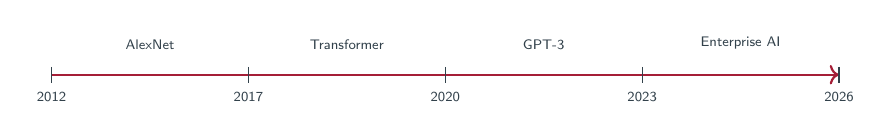
\begin{tikzpicture}
            \draw[->, thick, TuebingenRot] (0,0) -- (10,0);
            \foreach \x/\label in {0/2012, 2.5/2017, 5/2020, 7.5/2023, 10/2026} {
                \draw[TuebingenAnthrazit] (\x,0.1) -- (\x,-0.1) node[below] {\tiny\label};
            }
            \node[above, TuebingenAnthrazit] at (1.25,0.2) {\tiny AlexNet};
            \node[above, TuebingenAnthrazit] at (3.75,0.2) {\tiny Transformer};
            \node[above, TuebingenAnthrazit] at (6.25,0.2) {\tiny GPT-3};
            \node[above, TuebingenAnthrazit] at (8.75,0.2) {\tiny Enterprise AI};
        \end{tikzpicture}
    \end{center}
\end{frame}

% ==============================================================================
% 1.4 Full AI history timeline (12 slides with continuous timeline)
% ==============================================================================

% Define the timeline macro for consistent visualization across all slides
% Parameters: #1 = current era number (1-8)
\newcommand{\aitimeline}[1]{%
    \begin{tikzpicture}[remember picture]
        % Main timeline
        \draw[thick, TuebingenGray!50] (0,0) -- (11,0);
        
        % Era markers and labels
        \foreach \x/\era/\year/\label in {
            0.5/1/1940/A,
            2.0/2/1960/B,
            3.5/3/1970/C,
            5.0/4/1990/D,
            6.5/5/2006/E,
            8.0/6/2017/F,
            9.5/7/2020/G,
            11.0/8/2023/H%
        } {
            \ifnum\era=#1
                \fill[TuebingenRot] (\x,0) circle (5pt);
                \node[above=6pt, font=\tiny\bfseries, TuebingenRot] at (\x,0) {\year};
            \else
                \fill[TuebingenGray!40] (\x,0) circle (3pt);
                \node[above=4pt, font=\tiny, TuebingenGray] at (\x,0) {\year};
            \fi
        }
        
        % Era labels below
        \node[below=3pt, font=\tiny, TuebingenGray] at (0.5,0) {Found.};
        \node[below=3pt, font=\tiny, TuebingenGray] at (2.0,0) {Symb.};
        \node[below=3pt, font=\tiny, TuebingenGray] at (3.5,0) {Winter};
        \node[below=3pt, font=\tiny, TuebingenGray] at (5.0,0) {Stat.};
        \node[below=3pt, font=\tiny, TuebingenGray] at (6.5,0) {Deep};
        \node[below=3pt, font=\tiny, TuebingenGray] at (8.0,0) {Trans.};
        \node[below=3pt, font=\tiny, TuebingenGray] at (9.5,0) {Found.};
        \node[below=3pt, font=\tiny, TuebingenGray] at (11.0,0) {Now};
    \end{tikzpicture}%
}

% --- ERA A: Foundations (1940s–1960s) ---

\begin{frame}{The History of AI}
    \framesubtitle{Era A — Foundations (1940s–1960s)}
    
    \vspace{-0.3em}
    \begin{center}
        \aitimeline{1}
    \end{center}
    
    \vspace{0.5em}
    {\large\color{TuebingenRot}\textbf{The Birth of Artificial Intelligence}}
    
    \vspace{0.8em}
    \begin{columns}[T]
        \column{0.55\textwidth}
        \textbf{Key Milestones:}
        \begin{itemize}
            \setlength\itemsep{0.6em}
            \item \textbf{1943} — McCulloch \& Pitts: first neuron model \cite{mcculloch1943logical}
            \item \textbf{1950} — Turing's "Computing Machinery and Intelligence" \cite{turing1950computing}
            \item \textbf{1956} — Dartmouth: "AI" coined \cite{mccarthy1956dartmouth}
            \item \textbf{1958} — Rosenblatt's Perceptron \cite{rosenblatt1957perceptron}
        \end{itemize}
        
        \column{0.42\textwidth}
        \textbf{The Mood:}
        \begin{itemize}
            \setlength\itemsep{0.4em}
            \item Unbounded optimism
            \item "20 years to thinking machines"
            \item Heavy government funding
        \end{itemize}
        
        \vspace{0.8em}
        {\small\color{TuebingenGold}\textit{Lesson: Initial timelines were wildly optimistic.}}
    \end{columns}
\end{frame}

% --- ERA B: Symbolic AI (1960s–1970s) ---

\begin{frame}{The History of AI}
    \framesubtitle{Era B — Symbolic AI (1960s–1970s)}
    
    \vspace{-0.3em}
    \begin{center}
        \aitimeline{2}
    \end{center}
    
    \vspace{0.5em}
    {\large\color{TuebingenRot}\textbf{Logic-Based Reasoning}}
    
    \vspace{0.8em}
    \begin{columns}[T]
        \column{0.48\textwidth}
        \textbf{The Approach:}
        \begin{itemize}
            \setlength\itemsep{0.4em}
            \item Hand-coded expert rules
            \item Logic-based reasoning
            \item Knowledge representation
        \end{itemize}
        
        \column{0.48\textwidth}
        \textbf{1969 — Minsky \& Papert} \cite{minsky1969perceptrons}:
        \begin{itemize}
            \setlength\itemsep{0.4em}
            \item Critique of Perceptrons
            \item Showed fundamental limits
            \item Neural network funding collapsed
        \end{itemize}
    \end{columns}
    
    \vspace{0.8em}
    \begin{theorembox}{Why It Hit Limits}
        \textbf{Brittleness} — couldn't handle edge cases \quad | \quad \textbf{No learning} — couldn't improve from data
    \end{theorembox}
\end{frame}

% --- ERA C: AI Winters (1970s–1990s) - Split into 2 slides ---

\begin{frame}{The History of AI}
    \framesubtitle{Era C — First AI Winter (1974–1980)}
    
    \vspace{-0.3em}
    \begin{center}
        \aitimeline{3}
    \end{center}
    
    \vspace{0.5em}
    {\large\color{TuebingenRot}\textbf{Boom and Bust — Part I}}
    
    \vspace{0.8em}
    \begin{columns}[T]
        \column{0.48\textwidth}
        \textbf{The Collapse:}
        \begin{itemize}
            \setlength\itemsep{0.5em}
            \item DARPA cut funding after failed promises
            \item "AI can't deliver" sentiment spreads
            \item Research continued quietly in labs
        \end{itemize}
        
        \column{0.48\textwidth}
        \textbf{Expert Systems Boom (1980s):}
        \begin{itemize}
            \setlength\itemsep{0.5em}
            \item Commercial success initially
            \item XCON saved DEC \$40M/year
            \item Massive corporate investment
        \end{itemize}
    \end{columns}
    
    \vspace{1em}
    \begin{center}
        \color{TuebingenGold}\textbf{Pattern: Hype → Investment → Unmet expectations → Collapse}
    \end{center}
\end{frame}

\begin{frame}{The History of AI}
    \framesubtitle{Era C — Second AI Winter (1987–1993)}
    
    \vspace{-0.3em}
    \begin{center}
        \aitimeline{3}
    \end{center}
    
    \vspace{0.5em}
    {\large\color{TuebingenRot}\textbf{Boom and Bust — Part II}}
    
    \vspace{0.8em}
    \begin{columns}[T]
        \column{0.48\textwidth}
        \textbf{Why Expert Systems Failed:}
        \begin{itemize}
            \setlength\itemsep{0.5em}
            \item Expensive to maintain
            \item Rules became outdated quickly
            \item Couldn't adapt to change
            \item \$1B+ in failed projects
        \end{itemize}
        
        \column{0.48\textwidth}
        \textbf{Survivor Insight:}
        \begin{itemize}
            \setlength\itemsep{0.5em}
            \item The ideas weren't wrong
            \item Compute wasn't ready
            \item Data wasn't available
            \item Algorithms weren't mature
        \end{itemize}
    \end{columns}
    
    \vspace{1em}
    \begin{center}
        \color{TuebingenGreen}\textit{Sound familiar? The pattern would repeat.}
    \end{center}
\end{frame}

% --- ERA D: Statistical ML (1990s–2000s) ---

\begin{frame}{The History of AI}
    \framesubtitle{Era D — Statistical ML (1990s–2000s)}
    
    \vspace{-0.3em}
    \begin{center}
        \aitimeline{4}
    \end{center}
    
    \vspace{0.5em}
    {\large\color{TuebingenRot}\textbf{Learning from Data}}
    
    \vspace{0.8em}
    \begin{columns}[T]
        \column{0.48\textwidth}
        \textbf{Key Methods:}
        \begin{itemize}
            \setlength\itemsep{0.4em}
            \item Support Vector Machines \cite{cortes1995svm}
            \item Random Forests \cite{breiman2001randomforests}
            \item Boosting \cite{freund1997adaboost}
            \item Bayesian methods
        \end{itemize}
        
        \column{0.48\textwidth}
        \textbf{The Paradigm Shift:}
        \begin{itemize}
            \setlength\itemsep{0.4em}
            \item Don't encode rules — \textbf{learn patterns}
            \item More data → better models
            \item Practical: spam, fraud, recommendations
        \end{itemize}
    \end{columns}
    
    \vspace{0.8em}
    \begin{theorembox}{Executive Note}
        These techniques remain the right choice for many tabular/structured data problems today.
    \end{theorembox}
\end{frame}

% --- ERA E: Deep Learning (2006–2015) - Split into 2 slides ---

\begin{frame}{The History of AI}
    \framesubtitle{Era E — Deep Learning Revival (2006–2012)}
    
    \vspace{-0.3em}
    \begin{center}
        \aitimeline{5}
    \end{center}
    
    \vspace{0.5em}
    {\large\color{TuebingenRot}\textbf{Neural Networks Return}}
    
    \vspace{0.8em}
    \begin{columns}[T]
        \column{0.48\textwidth}
        \textbf{Key Breakthroughs:}
        \begin{itemize}
            \setlength\itemsep{0.5em}
            \item \textbf{2006} — Hinton's Deep Belief Networks \cite{hinton2006dbn}
            \item \textbf{2012} — \textcolor{TuebingenRot}{AlexNet} crushes ImageNet \cite{krizhevsky2012alexnet}
        \end{itemize}
        
        \column{0.48\textwidth}
        \textbf{What Changed:}
        \begin{itemize}
            \setlength\itemsep{0.5em}
            \item \textbf{GPUs} — 50× faster training
            \item \textbf{Big data} — ImageNet (14M images)
            \item \textbf{Open source} — reproducibility
        \end{itemize}
    \end{columns}
    
    \vspace{0.8em}
    \begin{theorembox}{The AlexNet Moment (2012)}
        Error rate dropped from 26\% to 15\% — a discontinuous leap proving deep learning works at scale.
    \end{theorembox}
\end{frame}

\begin{frame}{The History of AI}
    \framesubtitle{Era E — Deep Learning Expansion (2014–2015)}
    
    \vspace{-0.3em}
    \begin{center}
        \aitimeline{5}
    \end{center}
    
    \vspace{0.5em}
    {\large\color{TuebingenRot}\textbf{Going Deeper}}
    
    \vspace{0.8em}
    \begin{columns}[T]
        \column{0.48\textwidth}
        \textbf{Architecture Advances:}
        \begin{itemize}
            \setlength\itemsep{0.5em}
            \item \textbf{2014} — GANs \cite{goodfellow2014gan}
            \item \textbf{2015} — ResNet (152 layers!) \cite{he2016resnet}
            \item Dropout, batch norm, ReLU
        \end{itemize}
        
        \column{0.48\textwidth}
        \textbf{Key Lesson:}
        \begin{itemize}
            \setlength\itemsep{0.5em}
            \item When architecture + data + compute align...
            \item Progress can be sudden and dramatic
            \item Scale matters
        \end{itemize}
    \end{columns}
    
    \vspace{1em}
    \begin{center}
        \color{TuebingenGold}\textbf{The stage was set for language models.}
    \end{center}
\end{frame}

% --- ERA F: Transformers (2017–2020) - Split into 2 slides ---

\begin{frame}{The History of AI}
    \framesubtitle{Era F — The Transformer (2017)}
    
    \vspace{-0.3em}
    \begin{center}
        \aitimeline{6}
    \end{center}
    
    \vspace{0.5em}
    {\large\color{TuebingenRot}\textbf{"Attention Is All You Need"}}
    
    \vspace{0.8em}
    \begin{columns}[T]
        \column{0.48\textwidth}
        \textbf{The 2017 Paper} \cite{vaswani2017attention}:
        \begin{itemize}
            \setlength\itemsep{0.5em}
            \item Replaced sequential with parallel attention
            \item Enabled much larger models
            \item Better long-range dependencies
        \end{itemize}
        
        \column{0.48\textwidth}
        \textbf{What Followed:}
        \begin{itemize}
            \setlength\itemsep{0.5em}
            \item \textbf{2018} — BERT \cite{devlin2019bert}
            \item \textbf{2019} — GPT-2 \cite{radford2019gpt2}
            \item \textbf{2020} — GPT-3 \cite{brown2020gpt3}
        \end{itemize}
    \end{columns}
    
    \vspace{1em}
    \begin{center}
        \color{TuebingenGreen}\textbf{This is the architecture powering today's LLMs.}
    \end{center}
\end{frame}

\begin{frame}{The History of AI}
    \framesubtitle{Era F — Transfer Learning Paradigm (2018–2020)}
    
    \vspace{-0.3em}
    \begin{center}
        \aitimeline{6}
    \end{center}
    
    \vspace{0.5em}
    {\large\color{TuebingenRot}\textbf{Pretrain Once, Fine-tune Everywhere}}
    
    \vspace{0.8em}
    \begin{columns}[T]
        \column{0.48\textwidth}
        \textbf{The New Paradigm:}
        \begin{itemize}
            \setlength\itemsep{0.5em}
            \item Pretrain on massive text corpora
            \item Fine-tune for specific tasks
            \item Don't start from scratch
        \end{itemize}
        
        \column{0.48\textwidth}
        \textbf{Executive Implications:}
        \begin{itemize}
            \setlength\itemsep{0.5em}
            \item Language tasks suddenly tractable
            \item Foundation models as starting point
            \item Cost scales with model size
        \end{itemize}
    \end{columns}
    
    \vspace{0.8em}
    \begin{theorembox}{Key Insight}
        Context windows define capability limits. Larger context = more useful applications.
    \end{theorembox}
\end{frame}

% --- ERA G: Foundation Models (2020–2023) - Split into 2 slides ---

\begin{frame}{The History of AI}
    \framesubtitle{Era G — Foundation Models (2020–2022)}
    
    \vspace{-0.3em}
    \begin{center}
        \aitimeline{7}
    \end{center}
    
    \vspace{0.5em}
    {\large\color{TuebingenRot}\textbf{From Research to Products}}
    
    \vspace{0.8em}
    \begin{columns}[T]
        \column{0.48\textwidth}
        \textbf{Technical Advances:}
        \begin{itemize}
            \setlength\itemsep{0.5em}
            \item Instruction tuning \cite{ouyang2022instructgpt}
            \item RLHF — alignment with preferences
            \item Tool use — APIs, search, calculate
            \item Multimodal — text + images + code
        \end{itemize}
        
        \column{0.48\textwidth}
        \textbf{Key Releases:}
        \begin{itemize}
            \setlength\itemsep{0.5em}
            \item \textbf{ChatGPT} — 100M users in 2 months
            \item \textbf{GPT-4} \cite{openai2023gpt4} — multimodal
            \item \textbf{GitHub Copilot} — AI in IDEs
        \end{itemize}
    \end{columns}
    
    \vspace{1em}
    \begin{center}
        \color{TuebingenGold}\textbf{AI entered the mainstream consciousness.}
    \end{center}
\end{frame}

\begin{frame}{The History of AI}
    \framesubtitle{Era G — Enterprise Reality (2022–2023)}
    
    \vspace{-0.3em}
    \begin{center}
        \aitimeline{7}
    \end{center}
    
    \vspace{0.5em}
    {\large\color{TuebingenRot}\textbf{The Gap Between Demo and Production}}
    
    \vspace{0.8em}
    \begin{columns}[T]
        \column{0.48\textwidth}
        \textbf{Enterprise Challenges:}
        \begin{itemize}
            \setlength\itemsep{0.5em}
            \item Governance — who controls AI?
            \item Data privacy — where does data go?
            \item Integration — connecting to systems
            \item ROI — beyond demos to value
        \end{itemize}
        
        \column{0.48\textwidth}
        \textbf{Gaps Emerged:}
        \begin{itemize}
            \setlength\itemsep{0.5em}
            \item Demo-to-production is hard
            \item Hallucination is real
            \item Evaluation is immature
        \end{itemize}
    \end{columns}
    
    \vspace{0.8em}
    \begin{theorembox}{Executive Reality}
        The technology works. The challenge is making it work \textbf{reliably} in your context.
    \end{theorembox}
\end{frame}

% --- ERA H: Efficiency & Systems (2023–2026) - Split into 2 slides ---

\begin{frame}{The History of AI}
    \framesubtitle{Era H — Efficiency Revolution (2023–2024)}
    
    \vspace{-0.3em}
    \begin{center}
        \aitimeline{8}
    \end{center}
    
    \vspace{0.5em}
    {\large\color{TuebingenRot}\textbf{Better Models, Lower Costs}}
    
    \vspace{0.8em}
    \begin{columns}[T]
        \column{0.48\textwidth}
        \textbf{Efficiency Breakthroughs:}
        \begin{itemize}
            \setlength\itemsep{0.5em}
            \item Mixture-of-Experts \cite{jiang2024mixtral, deepseek2024moe}
            \item Distillation — small learns from large
            \item Quantization — less precision, same quality
        \end{itemize}
        
        \column{0.48\textwidth}
        \textbf{Open Models:}
        \begin{itemize}
            \setlength\itemsep{0.5em}
            \item Llama \cite{touvron2023llama}
            \item Mistral
            \item DeepSeek
            \item Self-hosting becomes viable
        \end{itemize}
    \end{columns}
    
    \vspace{1em}
    \begin{center}
        \color{TuebingenGreen}\textbf{Token costs dropped 100× in 2 years.}
    \end{center}
\end{frame}

\begin{frame}{The History of AI}
    \framesubtitle{Era H — Systems Discipline (2024–2026)}
    
    \vspace{-0.3em}
    \begin{center}
        \aitimeline{8}
    \end{center}
    
    \vspace{0.5em}
    {\large\color{TuebingenRot}\textbf{Where We Are Now}}
    
    \vspace{0.8em}
    \begin{columns}[T]
        \column{0.48\textwidth}
        \textbf{Systems Engineering:}
        \begin{itemize}
            \setlength\itemsep{0.5em}
            \item RAG \cite{lewis2020rag} — retrieval-augmented generation
            \item Evaluation discipline — measure first
            \item Workflow integration
            \item Agentic patterns with guardrails
        \end{itemize}
        
        \column{0.48\textwidth}
        \textbf{Executive Takeaway:}
        \begin{itemize}
            \setlength\itemsep{0.5em}
            \item Model selection = cost/capability trade-off
            \item Architecture > model size
            \item Evaluation is competitive advantage
        \end{itemize}
    \end{columns}
\end{frame}

\begin{frame}{Today's Reality}
    \framesubtitle{AI is a systems discipline, not just a model discipline.}
    
    \vspace{0.8em}
    \begin{theorembox}{Today's Reality}
        \textbf{AI is a systems discipline, not just a model discipline.}
    \end{theorembox}
\end{frame}

% ==============================================================================
% 1.5 Bridge: AI is a systems discipline now (1 slide)
% ==============================================================================

\begin{frame}{Bridge: AI Is a Systems Discipline Now}
    \framesubtitle{Setting up the deep dive}
    
    {\color{TuebingenGray} A working AI product is much more than a model.}
    
    \vspace{0.5em}
    \begin{center}
        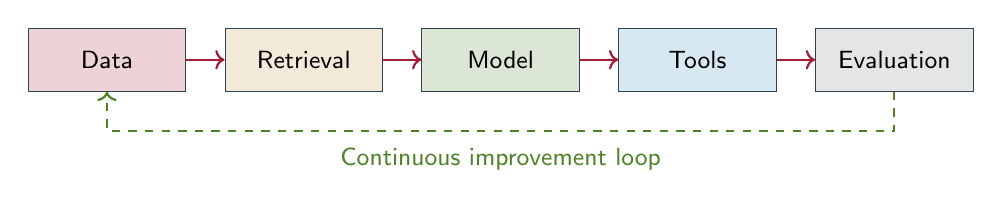
\begin{tikzpicture}[
            box/.style={rectangle, draw=TuebingenAnthrazit, fill=TuebingenBeige, minimum width=2cm, minimum height=0.8cm, align=center, font=\small},
            arrow/.style={->, thick, TuebingenRot}
        ]
            % Boxes
            \node[box, fill=TuebingenRot!20] (data) at (0,0) {Data};
            \node[box, fill=TuebingenGold!20] (retrieval) at (2.5,0) {Retrieval};
            \node[box, fill=TuebingenGreen!20] (model) at (5,0) {Model};
            \node[box, fill=TuebingenCyan!20] (tools) at (7.5,0) {Tools};
            \node[box, fill=TuebingenGray!20] (eval) at (10,0) {Evaluation};
            
            % Arrows
            \draw[arrow] (data) -- (retrieval);
            \draw[arrow] (retrieval) -- (model);
            \draw[arrow] (model) -- (tools);
            \draw[arrow] (tools) -- (eval);
            
            % Feedback loop
            \draw[arrow, TuebingenGreen, dashed] (eval.south) -- ++(0,-0.5) -| (data.south);
            
            % Label
            \node[below, TuebingenGreen] at (5,-1) {\small Continuous improvement loop};
        \end{tikzpicture}
    \end{center}
    
    \vspace{0.3em}
    \begin{columns}[T]
        \column{0.48\textwidth}
        \textbf{The Full Stack:}
        \begin{itemize}
            \setlength\itemsep{0.2em}
            \item Data pipelines \& quality
            \item Retrieval \& knowledge systems
            \item Model selection \& prompting
            \item Tool integration \& guardrails
            \item Evaluation \& monitoring
        \end{itemize}
        
        \column{0.48\textwidth}
        \textbf{What This Means for You:}
        \begin{itemize}
            \setlength\itemsep{0.2em}
            \item Don't just "buy a model"
            \item Invest in data \& evaluation
            \item Architect for iteration
            \item Govern the whole system
        \end{itemize}
    \end{columns}
\end{frame}

% Act II — How Modern AI Works (2 hours deep dive)
\section{How Modern AI Works}

% ==============================================================================
% PART II-A: ML TAXONOMY AND CLASSICAL METHODS (30 minutes)
% ==============================================================================

% ------------------------------------------------------------------------------
% II-A.1 Types of ML: supervised, unsupervised, RL (3 slides)
% ------------------------------------------------------------------------------

\begin{frame}{The Three Paradigms of Machine Learning}
    \framesubtitle{How machines learn from data}
    
    {\color{TuebingenGray} All ML methods fall into three fundamental learning paradigms—each suited to different business problems.}
    
    \vspace{0.8em}
    \begin{columns}[T]
        \column{0.32\textwidth}
        \begin{center}
            {\Large \color{TuebingenRot} \textbf{Supervised}}\\[0.3em]
            {\small Learning from labeled examples}
        \end{center}
        \vspace{0.3em}
        \begin{itemize}
            \setlength\itemsep{0.2em}
            \item Input → Known output
            \item Learn the mapping
            \item Predict on new data
        \end{itemize}
        \vspace{0.3em}
        {\scriptsize\color{TuebingenGray} Classification, regression, forecasting}
        
        \column{0.32\textwidth}
        \begin{center}
            {\Large \color{TuebingenGold} \textbf{Unsupervised}}\\[0.3em]
            {\small Finding structure in data}
        \end{center}
        \vspace{0.3em}
        \begin{itemize}
            \setlength\itemsep{0.2em}
            \item No labels provided
            \item Discover patterns
            \item Group similar items
        \end{itemize}
        \vspace{0.3em}
        {\scriptsize\color{TuebingenGray} Clustering, anomaly detection, compression}
        
        \column{0.32\textwidth}
        \begin{center}
            {\Large \color{TuebingenGreen} \textbf{Reinfortic Learning}}\\[0.3em]
            {\small Learning from rewards}
        \end{center}
        \vspace{0.3em}
        \begin{itemize}
            \setlength\itemsep{0.2em}
            \item Sequential decisions
            \item Trial and error
            \item Maximize long-term reward
        \end{itemize}
        \vspace{0.3em}
        {\scriptsize\color{TuebingenGray} Games, robotics, recommendations}
    \end{columns}
    
    \vspace{0.8em}
    \begin{center}
        \small\color{TuebingenRot} \textbf{Executive insight:} 90\%+ of enterprise ML is supervised learning on structured data.
    \end{center}
\end{frame}

\begin{frame}{Supervised Learning: The Workhorse of Enterprise AI}
    \framesubtitle{Classification and regression}
    
    {\color{TuebingenGray} Most business AI problems are supervised: you have historical data with known outcomes.}
    
    \vspace{0.3em}
    \begin{columns}[T]
        \column{0.48\textwidth}
        {\color{TuebingenRot}\textbf{Classification} — Discrete categories}
        \begin{itemize}
            \setlength\itemsep{0.2em}
            \item Will this customer churn? {\scriptsize (Yes/No)}
            \item Is this transaction fraud? {\scriptsize (Yes/No)}
            \item What topic is this email? {\scriptsize (Sales/Support/Spam)}
            \item Which product to recommend? {\scriptsize (A/B/C/...)}
        \end{itemize}
        
        \vspace{0.3em}
        {\small\color{TuebingenGray} Output: probabilities across categories}
        
        \column{0.48\textwidth}
        {\color{TuebingenGold}\textbf{Regression} — Continuous values}
        \begin{itemize}
            \setlength\itemsep{0.2em}
            \item What will revenue be next quarter?
            \item How long until this machine fails?
            \item What price maximizes profit?
            \item How many units will we sell?
        \end{itemize}
        
        \vspace{0.3em}
        {\small\color{TuebingenGray} Output: a number (with uncertainty)}
    \end{columns}
    
    \vspace{0.3em}
    \begin{theorembox}{The Supervised Learning Recipe}
        \textbf{1.} Collect historical data with known outcomes (labels) \\
        \textbf{2.} Train model to find patterns connecting inputs to outputs \\
        \textbf{3.} Validate on held-out data to estimate real-world performance \\
        \textbf{4.} Deploy and monitor for drift
    \end{theorembox}
\end{frame}

\begin{frame}{Unsupervised \& Reinforcement Learning}
    \framesubtitle{When labels are unavailable or actions matter}
    
    \vspace{0.3em}
    \begin{columns}[T]
        \column{0.48\textwidth}
        {\color{TuebingenGold}\textbf{Unsupervised Learning}}
        
        \vspace{0.3em}
        {\small No labels—find structure in data itself}
        
        \vspace{0.3em}
        \textbf{Key techniques:}
        \begin{itemize}
            \setlength\itemsep{0.3em}
            \item \textbf{Clustering} — group similar customers, documents, behaviors
            \item \textbf{Dimensionality reduction} — compress features, visualize high-dim data (PCA, t-SNE)
            \item \textbf{Anomaly detection} — find outliers without labeled fraud cases
        \end{itemize}
        
        \vspace{0.3em}
        {\scriptsize\color{TuebingenGray} \textbf{Use when:} You don't have labels, or want to discover unknown patterns}
        
        \column{0.48\textwidth}
        {\color{TuebingenGreen}\textbf{Reinforcement Learning (RL)}}
        
        \vspace{0.3em}
        {\small Learn optimal actions through trial and error}
        
        \vspace{0.3em}
        \textbf{Key characteristics:}
        \begin{itemize}
            \setlength\itemsep{0.3em}
            \item \textbf{Sequential decisions} — actions affect future states
            \item \textbf{Delayed rewards} — outcome known only later
            \item \textbf{Exploration vs exploitation} — try new vs use known
        \end{itemize}
        
        \vspace{0.3em}
        {\scriptsize\color{TuebingenGray} \textbf{Use when:} Optimizing multi-step processes (pricing, routing, control)}
    \end{columns}
    
    \vspace{0.5em}
    \begin{center}
        \small\color{TuebingenRot} \textbf{Note:} RL is powerful but harder to productize. Start with supervised if you have labels.
    \end{center}
\end{frame}

% ------------------------------------------------------------------------------
% II-A.2 MLPs: the baseline neural network (2 slides + example)
% ------------------------------------------------------------------------------

\begin{frame}{Multi-Layer Perceptrons (MLPs): The Foundation}
    \framesubtitle{The simplest neural network architecture}
    
    {\color{TuebingenGray} An MLP is a stack of layers that learn to transform inputs into outputs through nonlinear functions.}
    
    \vspace{0.5em}
    \begin{columns}[T]
        \column{0.45\textwidth}
        \begin{center}
            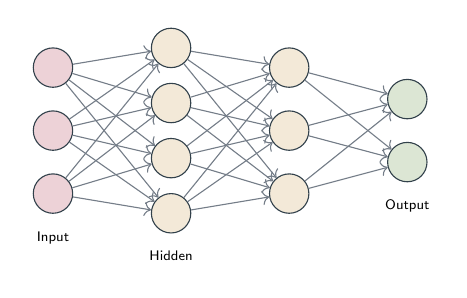
\begin{tikzpicture}[
                neuron/.style={circle, draw=TuebingenAnthrazit, minimum size=0.5cm, fill=TuebingenBeige},
                input/.style={neuron, fill=TuebingenRot!20},
                hidden/.style={neuron, fill=TuebingenGold!20},
                output/.style={neuron, fill=TuebingenGreen!20},
                conn/.style={->, TuebingenGray, thin}
            ]
                % Input layer
                \foreach \i in {1,2,3} {
                    \node[input] (i\i) at (0, -\i*0.8+1.6) {};
                }
                \node[below=0.1cm of i3, font=\tiny] {Input};
                
                % Hidden layer 1
                \foreach \i in {1,2,3,4} {
                    \node[hidden] (h1\i) at (1.5, -\i*0.7+1.75) {};
                }
                \node[below=0.1cm of h14, font=\tiny] {Hidden};
                
                % Hidden layer 2
                \foreach \i in {1,2,3} {
                    \node[hidden] (h2\i) at (3, -\i*0.8+1.6) {};
                }
                
                % Output layer
                \foreach \i in {1,2} {
                    \node[output] (o\i) at (4.5, -\i*0.8+1.2) {};
                }
                \node[below=0.1cm of o2, font=\tiny] {Output};
                
                % Connections (simplified)
                \foreach \i in {1,2,3} {
                    \foreach \j in {1,2,3,4} {
                        \draw[conn] (i\i) -- (h1\j);
                    }
                }
                \foreach \i in {1,2,3,4} {
                    \foreach \j in {1,2,3} {
                        \draw[conn] (h1\i) -- (h2\j);
                    }
                }
                \foreach \i in {1,2,3} {
                    \foreach \j in {1,2} {
                        \draw[conn] (h2\i) -- (o\j);
                    }
                }
            \end{tikzpicture}
        \end{center}
        
        \column{0.52\textwidth}
        \textbf{How it works:}
        \begin{itemize}
            \setlength\itemsep{0.3em}
            \item Each connection has a learnable \textbf{weight}
            \item Each layer applies: $\text{output} = \sigma(Wx + b)$
            \item $\sigma$ is a nonlinearity (ReLU, sigmoid)
            \item \textbf{Training:} adjust weights to minimize prediction error
        \end{itemize}
        
        \vspace{0.3em}
        \textbf{Key insight:}
        \begin{itemize}
            \setlength\itemsep{0.2em}
            \item Can approximate \textit{any} function (universal approximation)
            \item More layers = more expressive power
            \item But: needs lots of data to avoid overfitting
        \end{itemize}
    \end{columns}
\end{frame}

\begin{frame}{MLPs in Practice: When to Use Them}
    \framesubtitle{Strengths, weaknesses, and enterprise applications}
    
    \vspace{0.3em}
    \begin{columns}[T]
        \column{0.48\textwidth}
        {\color{TuebingenGreen}\textbf{Strengths:}}
        \begin{itemize}
            \setlength\itemsep{0.3em}
            \item Flexible function approximation
            \item Works on \textbf{tabular data} (structured)
            \item Easy to implement and train
            \item Foundation for all deep learning
        \end{itemize}
        
        \vspace{0.5em}
        {\color{TuebingenRot}\textbf{Weaknesses:}}
        \begin{itemize}
            \setlength\itemsep{0.3em}
            \item Often \textbf{outperformed by tree-based methods} on tabular data (XGBoost, Random Forest)
            \item No built-in structure for images, text, sequences
            \item Can overfit without regularization
        \end{itemize}
        
        \column{0.48\textwidth}
        \textbf{Enterprise Use Cases:}
        \begin{itemize}
            \setlength\itemsep{0.4em}
            \item \textbf{Churn prediction} — customer features → churn probability
            \item \textbf{Credit scoring} — financial data → risk score
            \item \textbf{Demand forecasting} — historical features → units sold
            \item \textbf{Fraud detection} — transaction features → fraud probability
        \end{itemize}
        
        \vspace{0.5em}
        \begin{center}
            \small\color{TuebingenGray}
            \fbox{\parbox{0.9\linewidth}{\centering
                \textbf{Executive rule:}\\
                For tabular data, try gradient-boosted trees (XGBoost) first—often better with less tuning.
            }}
        \end{center}
    \end{columns}
\end{frame}

% ------------------------------------------------------------------------------
% II-A.3 PCA: dimensionality reduction (2 slides + example)
% ------------------------------------------------------------------------------

\begin{frame}{PCA: Dimensionality Reduction}
    \framesubtitle{Compressing data while preserving information}
    
    {\color{TuebingenGray} Principal Component Analysis (PCA) finds the directions of maximum variance in your data.}
    
    \vspace{0.5em}
    \begin{columns}[T]
        \column{0.45\textwidth}
        \begin{center}
            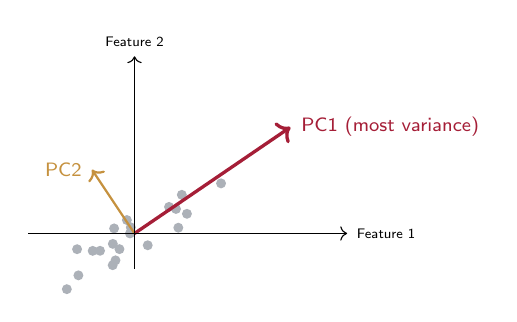
\begin{tikzpicture}[scale=0.9]
                % Data points (scattered)
                \foreach \i in {1,...,20} {
                    \pgfmathsetmacro{\x}{0.8*rand + 0.5*rand}
                    \pgfmathsetmacro{\y}{0.6*\x + 0.3*rand}
                    \fill[TuebingenGray!60] (\x, \y) circle (2pt);
                }
                
                % Principal components
                \draw[->, very thick, TuebingenRot] (0,0) -- (2.2, 1.5) node[right, font=\scriptsize] {PC1 (most variance)};
                \draw[->, thick, TuebingenGold] (0,0) -- (-0.6, 0.9) node[left, font=\scriptsize] {PC2};
                
                % Axes
                \draw[->] (-1.5,0) -- (3,0) node[right, font=\tiny] {Feature 1};
                \draw[->] (0,-0.5) -- (0,2.5) node[above, font=\tiny] {Feature 2};
            \end{tikzpicture}
        \end{center}
        {\small\centering Original: 2 dimensions\\PCA finds directions of spread}
        
        \column{0.52\textwidth}
        \textbf{What PCA Does:}
        \begin{itemize}
            \setlength\itemsep{0.3em}
            \item Finds \textbf{orthogonal axes} (principal components)
            \item Ranked by \textbf{variance explained}
            \item Project data onto top $k$ components
            \item \textbf{Lossy compression}: keep signal, reduce noise
        \end{itemize}
        
        \vspace{0.3em}
        \textbf{Use Cases:}
        \begin{itemize}
            \setlength\itemsep{0.2em}
            \item Reduce 1000 features to 50 for faster training
            \item Visualize high-dimensional data in 2D/3D
            \item Remove noise from sensor data
            \item Feature engineering before ML
        \end{itemize}
    \end{columns}
    
    \vspace{0.3em}
    \begin{center}
        \small\color{TuebingenRot} \textbf{Limitation:} PCA only captures \textit{linear} relationships.
    \end{center}
\end{frame}

\begin{frame}{PCA Example: Customer Behavior Analysis}
    \framesubtitle{From 50 metrics to actionable segments}
    
    \vspace{0.3em}
    \begin{columns}[T]
        \column{0.48\textwidth}
        \textbf{The Scenario:}
        \begin{itemize}
            \setlength\itemsep{0.3em}
            \item Marketing has 50 customer metrics
            \item Purchase frequency, recency, categories, channel preferences, engagement scores...
            \item Too many dimensions to visualize or interpret
        \end{itemize}
        
        \vspace{0.3em}
        \textbf{PCA Reveals:}
        \begin{itemize}
            \setlength\itemsep{0.3em}
            \item \textbf{PC1} (40\% variance): "Overall engagement"
            \item \textbf{PC2} (15\% variance): "Price sensitivity"
            \item \textbf{PC3} (10\% variance): "Channel preference"
            \item First 3 components capture 65\% of information
        \end{itemize}
        
        \column{0.48\textwidth}
        \begin{center}
            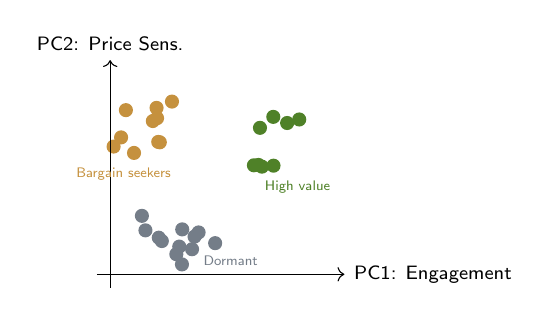
\begin{tikzpicture}[scale=0.85]
                % Simulated customer clusters in 2D PCA space
                % Cluster 1: High value
                \foreach \i in {1,...,8} {
                    \pgfmathsetmacro{\x}{2.5 + 0.4*rand}
                    \pgfmathsetmacro{\y}{2 + 0.4*rand}
                    \fill[TuebingenGreen] (\x, \y) circle (3pt);
                }
                % Cluster 2: Price sensitive
                \foreach \i in {1,...,10} {
                    \pgfmathsetmacro{\x}{0.5 + 0.5*rand}
                    \pgfmathsetmacro{\y}{2.2 + 0.4*rand}
                    \fill[TuebingenGold] (\x, \y) circle (3pt);
                }
                % Cluster 3: Low engagement
                \foreach \i in {1,...,12} {
                    \pgfmathsetmacro{\x}{1 + 0.6*rand}
                    \pgfmathsetmacro{\y}{0.5 + 0.4*rand}
                    \fill[TuebingenGray] (\x, \y) circle (3pt);
                }
                
                % Axes
                \draw[->] (-0.2,0) -- (3.5,0) node[right, font=\scriptsize] {PC1: Engagement};
                \draw[->] (0,-0.2) -- (0,3.2) node[above, font=\scriptsize] {PC2: Price Sens.};
                
                % Labels
                \node[font=\tiny, TuebingenGreen] at (2.8, 1.3) {High value};
                \node[font=\tiny, TuebingenGold] at (0.2, 1.5) {Bargain seekers};
                \node[font=\tiny, TuebingenGray] at (1.8, 0.2) {Dormant};
            \end{tikzpicture}
        \end{center}
        
        \vspace{0.3em}
        {\small\color{TuebingenGray} \textbf{Result:} Clear segments emerge from compressed representation}
    \end{columns}
    
    \vspace{0.3em}
    \begin{center}
        \small\color{TuebingenRot} \textbf{Caveat:} Components are interpretable only if you examine the loadings (which original features contribute).
    \end{center}
\end{frame}

% ------------------------------------------------------------------------------
% II-A.4 t-SNE: local neighborhood visualization (2 slides + example)
% ------------------------------------------------------------------------------

\begin{frame}{t-SNE: Visualizing Complex Data}
    \framesubtitle{Nonlinear dimensionality reduction for exploration}
    
    {\color{TuebingenGray} t-SNE (t-distributed Stochastic Neighbor Embedding) preserves \textit{local neighborhoods} when projecting to 2D.}
    
    \vspace{0.5em}
    \begin{columns}[T]
        \column{0.48\textwidth}
        \textbf{How t-SNE Differs from PCA:}
        \begin{itemize}
            \setlength\itemsep{0.4em}
            \item \textbf{PCA:} Linear projection, preserves global variance
            \item \textbf{t-SNE:} Nonlinear, preserves \textit{local similarity}
            \item Points that are similar stay close
            \item Reveals \textbf{clusters} that PCA might miss
        \end{itemize}
        
        \vspace{0.3em}
        \textbf{Use Cases:}
        \begin{itemize}
            \setlength\itemsep{0.3em}
            \item Visualizing embeddings (words, documents, images)
            \item Exploring customer segments
            \item Quality check on clustering results
        \end{itemize}
        
        \column{0.48\textwidth}
        \begin{center}
            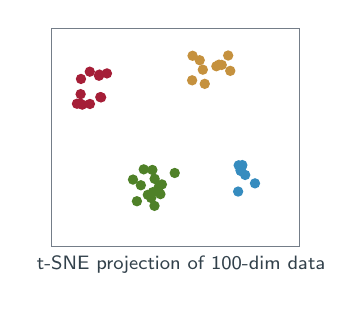
\begin{tikzpicture}[scale=0.75]
                % Simulated t-SNE clusters (more separated than PCA)
                % Cluster 1
                \foreach \i in {1,...,12} {
                    \pgfmathsetmacro{\x}{0.5 + 0.3*rand}
                    \pgfmathsetmacro{\y}{2.5 + 0.3*rand}
                    \fill[TuebingenRot] (\x, \y) circle (2.5pt);
                }
                % Cluster 2
                \foreach \i in {1,...,10} {
                    \pgfmathsetmacro{\x}{2.5 + 0.35*rand}
                    \pgfmathsetmacro{\y}{2.8 + 0.25*rand}
                    \fill[TuebingenGold] (\x, \y) circle (2.5pt);
                }
                % Cluster 3
                \foreach \i in {1,...,14} {
                    \pgfmathsetmacro{\x}{1.5 + 0.4*rand}
                    \pgfmathsetmacro{\y}{0.8 + 0.35*rand}
                    \fill[TuebingenGreen] (\x, \y) circle (2.5pt);
                }
                % Cluster 4
                \foreach \i in {1,...,8} {
                    \pgfmathsetmacro{\x}{3.2 + 0.25*rand}
                    \pgfmathsetmacro{\y}{1 + 0.3*rand}
                    \fill[TuebingenCyan] (\x, \y) circle (2.5pt);
                }
                
                % Frame
                \draw[TuebingenGray, thin] (-0.2,-0.2) rectangle (4,3.5);
                \node[font=\scriptsize, TuebingenAnthrazit] at (2, -0.5) {t-SNE projection of 100-dim data};
            \end{tikzpicture}
        \end{center}
        {\small\centering Clusters clearly separated}
    \end{columns}
\end{frame}

\begin{frame}{t-SNE: Critical Warnings for Executives}
    \framesubtitle{What t-SNE cannot tell you}
    
    \vspace{0.3em}
    \begin{columns}[T]
        \column{0.55\textwidth}
        {\color{TuebingenRot}\textbf{t-SNE is NOT:}}
        \begin{itemize}
            \setlength\itemsep{0.5em}
            \item \textbf{Distance-preserving} — distances between clusters are meaningless
            \item \textbf{Deterministic} — different runs give different layouts
            \item \textbf{A clustering algorithm} — it only visualizes, doesn't assign labels
            \item \textbf{Suitable for quantitative analysis} — don't measure cluster sizes/gaps
        \end{itemize}
        
        \vspace{0.5em}
        {\color{TuebingenGreen}\textbf{t-SNE IS:}}
        \begin{itemize}
            \setlength\itemsep{0.3em}
            \item Great for \textbf{exploration} and hypothesis generation
            \item Useful to \textbf{sanity-check} other analyses
            \item A way to \textbf{communicate} structure visually
        \end{itemize}
        
        \column{0.42\textwidth}
        \begin{theorembox}{Executive Rule}
            Use t-SNE for \textbf{qualitative exploration only}.
            
            \vspace{0.3em}
            
            {\small Never make business decisions based on:}
            \begin{itemize}
                \item Cluster sizes in t-SNE plots
                \item Distances between clusters
                \item Apparent "gaps" in the data
            \end{itemize}
            
            \vspace{0.3em}
            
            {\small Always validate with quantitative methods.}
        \end{theorembox}
    \end{columns}
    
    \vspace{0.3em}
    \begin{center}
        \small\color{TuebingenGray} \textbf{Modern alternative:} UMAP—faster and better preserves global structure, but same caveats apply.
    \end{center}
\end{frame}

% ------------------------------------------------------------------------------
% II-A.5 CNNs: why they mattered and where they still matter (2 slides + example)
% ------------------------------------------------------------------------------

\begin{frame}{Convolutional Neural Networks (CNNs)}
    \framesubtitle{The architecture that conquered computer vision}
    
    {\color{TuebingenGray} CNNs revolutionized image processing by learning spatial hierarchies of features.}
    
    \vspace{0.3em}
    \begin{columns}[T]
        \column{0.50\textwidth}
        \textbf{Key Innovation:}
        \begin{itemize}
            \setlength\itemsep{0.3em}
            \item \textbf{Local receptive fields} — each neuron sees only a small patch
            \item \textbf{Weight sharing} — same filter applied everywhere
            \item \textbf{Hierarchical features} — edges → shapes → objects
            \item Far fewer parameters than fully connected
        \end{itemize}
        
        \vspace{0.3em}
        \textbf{The AlexNet Moment (2012)} \cite{krizhevsky2012alexnet}:
        \begin{itemize}
            \setlength\itemsep{0.2em}
            \item ImageNet error: 26\% → 15\%
            \item Discontinuous improvement
            \item CNN + GPU + Big Data = breakthrough
        \end{itemize}
        
        \column{0.47\textwidth}
        \begin{center}
            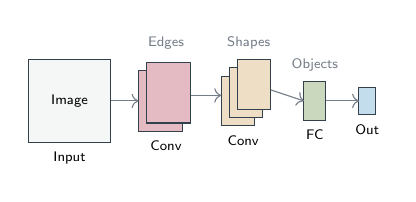
\begin{tikzpicture}[scale=0.7]
                % Input image
                \draw[fill=TuebingenBeige, draw=TuebingenAnthrazit] (0,0) rectangle (1.5,1.5);
                \node[font=\tiny] at (0.75, 0.75) {Image};
                \node[font=\tiny, below] at (0.75, 0) {Input};
                
                % Conv layers (progressively smaller, deeper)
                \draw[fill=TuebingenRot!30, draw=TuebingenAnthrazit] (2,0.2) rectangle (2.8,1.3);
                \draw[fill=TuebingenRot!30, draw=TuebingenAnthrazit] (2.15,0.35) rectangle (2.95,1.45);
                \node[font=\tiny, below] at (2.5, 0.2) {Conv};
                
                \draw[fill=TuebingenGold!30, draw=TuebingenAnthrazit] (3.5,0.3) rectangle (4.1,1.2);
                \draw[fill=TuebingenGold!30, draw=TuebingenAnthrazit] (3.65,0.45) rectangle (4.25,1.35);
                \draw[fill=TuebingenGold!30, draw=TuebingenAnthrazit] (3.8,0.6) rectangle (4.4,1.5);
                \node[font=\tiny, below] at (3.9, 0.3) {Conv};
                
                % Fully connected
                \draw[fill=TuebingenGreen!30, draw=TuebingenAnthrazit] (5,0.4) rectangle (5.4,1.1);
                \node[font=\tiny, below] at (5.2, 0.4) {FC};
                
                % Output
                \draw[fill=TuebingenCyan!30, draw=TuebingenAnthrazit] (6,0.5) rectangle (6.3,1);
                \node[font=\tiny, below] at (6.15, 0.5) {Out};
                
                % Arrows
                \draw[->, TuebingenGray] (1.5, 0.75) -- (2, 0.75);
                \draw[->, TuebingenGray] (2.95, 0.85) -- (3.5, 0.85);
                \draw[->, TuebingenGray] (4.4, 0.95) -- (5, 0.75);
                \draw[->, TuebingenGray] (5.4, 0.75) -- (6, 0.75);
                
                % Labels
                \node[font=\tiny, TuebingenGray] at (2.5, 1.8) {Edges};
                \node[font=\tiny, TuebingenGray] at (4, 1.8) {Shapes};
                \node[font=\tiny, TuebingenGray] at (5.2, 1.4) {Objects};
            \end{tikzpicture}
        \end{center}
        
        \vspace{0.3em}
        {\small\color{TuebingenGray} \textbf{Insight:} CNN layers learn increasingly abstract features automatically.}
    \end{columns}
\end{frame}

\begin{frame}{CNNs in Enterprise: Where They Still Dominate}
    \framesubtitle{Practical applications beyond research}
    
    \vspace{0.2em}
    \begin{columns}[T]
        \column{0.48\textwidth}
        \textbf{Manufacturing \& Quality:}
        \begin{itemize}
            \setlength\itemsep{0.2em}
            \item \textbf{Defect detection} — visual inspection at scale
            \item \textbf{Quality control} — surface anomalies, assembly verification
            \item \textbf{Predictive maintenance} — analyze equipment images
        \end{itemize}
        
        \vspace{0.2em}
        \textbf{Document Processing:}
        \begin{itemize}
            \setlength\itemsep{0.2em}
            \item \textbf{OCR} — text extraction from images
            \item \textbf{Document classification} — invoices, receipts, forms
            \item \textbf{Signature verification}
        \end{itemize}
        
        \column{0.48\textwidth}
        \textbf{Healthcare \& Medical:}
        \begin{itemize}
            \setlength\itemsep{0.2em}
            \item \textbf{Medical imaging} — X-rays, MRIs, pathology slides
            \item \textbf{Diagnostic assistance} — detect anomalies, measure features
        \end{itemize}
        
        \vspace{0.2em}
        \textbf{Retail \& Security:}
        \begin{itemize}
            \setlength\itemsep{0.2em}
            \item \textbf{Visual search} — find similar products
            \item \textbf{Inventory tracking} — shelf monitoring
            \item \textbf{Access control} — facial recognition
        \end{itemize}
    \end{columns}
    
\end{frame}

\begin{frame}{Executive Lesson from CNNs}
    \vspace{0.3em}
    \begin{theorembox}{Executive Lesson from CNNs}
        The AlexNet breakthrough taught us: when \textbf{architecture} + \textbf{data} + \textbf{compute} align, progress can be \textbf{sudden and dramatic}. This pattern repeated with Transformers in 2017.
    \end{theorembox}
\end{frame}

% ==============================================================================
% PART II-B: DEEP LEARNING BUILDING BLOCKS (30 minutes)
% ==============================================================================

% ------------------------------------------------------------------------------
% II-B.1 Representations: what the network "learns" (1 slide)
% ------------------------------------------------------------------------------

\begin{frame}{What Neural Networks Actually Learn}
    \framesubtitle{Representations are the key insight}
    
    {\color{TuebingenGray} The magic of deep learning: networks learn to \textit{represent} data, not just classify it.}
    
    \vspace{0.3em}
    \begin{columns}[T]
        \column{0.48\textwidth}
        \textbf{Traditional ML:}
        \begin{itemize}
            \setlength\itemsep{0.3em}
            \item Humans engineer features
            \item "Age, income, purchase count..."
            \item Model learns \textit{weights} on fixed features
            \item Quality depends on feature design
        \end{itemize}
        
        \vspace{0.3em}
        {\color{TuebingenGray}\small Feature engineering is manual and domain-specific}
        
        \column{0.48\textwidth}
        \textbf{Deep Learning:}
        \begin{itemize}
            \setlength\itemsep{0.3em}
            \item Network learns features automatically
            \item Hidden layers = learned representations
            \item "Embedding" = useful compressed form
            \item Transfers across tasks
        \end{itemize}
        
        \vspace{0.3em}
        {\color{TuebingenGreen}\small Representation learning scales with data}
    \end{columns}
    
    \vspace{0.5em}
    \begin{theorembox}{Key Insight}
        The \textbf{representation layer} (embeddings) is often more valuable than the final output. \\
        A good representation can be reused for many downstream tasks.
    \end{theorembox}
\end{frame}

% ------------------------------------------------------------------------------
% II-B.2 Autoencoders: encoder/decoder explained (3 slides + example)
% ------------------------------------------------------------------------------

\begin{frame}{Autoencoders: Learning to Compress}
    \framesubtitle{The encoder-decoder architecture}
    
    {\color{TuebingenGray} An autoencoder learns to compress data into a small representation, then reconstruct it.}
    
    \vspace{0.5em}
    \begin{columns}[T]
        \column{0.50\textwidth}
        \begin{center}
            \includegraphics[width=\textwidth]{acts/act2_modern_ai/figures/autoencoder_implementation.png}
        \end{center}
        
        \column{0.47\textwidth}
        \textbf{How It Works:}
        \begin{itemize}
            \setlength\itemsep{0.3em}
            \item \textbf{Encoder:} Compress input to small "latent" vector
            \item \textbf{Bottleneck:} Forces network to learn essential features
            \item \textbf{Decoder:} Reconstruct original from latent
            \item \textbf{Training:} Minimize reconstruction error
        \end{itemize}
        
        \vspace{0.3em}
        \textbf{The Insight:}
        \begin{itemize}
            \setlength\itemsep{0.2em}
            \item If it can reconstruct, latent must capture meaning
            \item Latent = compressed representation
        \end{itemize}
    \end{columns}
\end{frame}

\begin{frame}{Autoencoder Applications}
    \framesubtitle{Compression, denoising, and anomaly detection}
    
    \vspace{0.3em}
    \begin{columns}[T]
        \column{0.32\textwidth}
        \begin{center}
            {\color{TuebingenRot}\textbf{Compression}}
        \end{center}
        \vspace{0.2em}
        \begin{itemize}
            \setlength\itemsep{0.2em}
            \item Reduce data dimensionality
            \item Store latent vectors instead of raw data
            \item Faster downstream processing
        \end{itemize}
        \vspace{0.3em}
        {\scriptsize\color{TuebingenGray} Example: Compress 1000 features to 50}
        
        \column{0.32\textwidth}
        \begin{center}
            {\color{TuebingenGold}\textbf{Denoising}}
        \end{center}
        \vspace{0.2em}
        \begin{itemize}
            \setlength\itemsep{0.2em}
            \item Train on noisy → clean pairs
            \item Network learns to remove noise
            \item Extracts underlying signal
        \end{itemize}
        \vspace{0.3em}
        {\scriptsize\color{TuebingenGray} Example: Clean sensor data, audio}
        
        \column{0.32\textwidth}
        \begin{center}
            {\color{TuebingenGreen}\textbf{Anomaly Detection}}
        \end{center}
        \vspace{0.2em}
        \begin{itemize}
            \setlength\itemsep{0.2em}
            \item Train only on "normal" data
            \item Anomalies = high reconstruction error
            \item No labeled anomalies needed!
        \end{itemize}
        \vspace{0.3em}
        {\scriptsize\color{TuebingenGray} Example: Fraud, equipment failure}
    \end{columns}
    
    \vspace{0.5em}
    \begin{theorembox}{Anomaly Detection Pattern}
        \textbf{1.} Train autoencoder on normal operations only \\
        \textbf{2.} In production: if reconstruction error > threshold → flag as anomaly \\
        \textbf{3.} \textit{Key advantage:} Works without labeled fraud/failure cases
    \end{theorembox}
\end{frame}

\begin{frame}{Autoencoder Example: Industrial Anomaly Detection}
    \framesubtitle{Detecting equipment failures without labeled failure data}
    
    \vspace{0.3em}
    \begin{columns}[T]
        \column{0.48\textwidth}
        \textbf{The Scenario:}
        \begin{itemize}
            \setlength\itemsep{0.3em}
            \item Manufacturing equipment with 100 sensors
            \item Failures are rare (good!)
            \item But: no labeled failure data to train on
            \item Need: early warning system
        \end{itemize}
        
        \vspace{0.3em}
        \textbf{Autoencoder Solution:}
        \begin{itemize}
            \setlength\itemsep{0.3em}
            \item Train on months of \textit{normal} operation
            \item Network learns "what normal looks like"
            \item Pre-failure: sensors drift from normal
            \item Autoencoder can't reconstruct abnormal patterns
            \item High error = early warning
        \end{itemize}
        
        \column{0.48\textwidth}
        \begin{center}
            \includegraphics[width=\textwidth]{acts/act2_modern_ai/figures/autoencoder_representation.png}
        \end{center}
        
        \vspace{0.3em}
        {\small\color{TuebingenGray} \textbf{Geometric view:} The encoder maps data to a lower-dimensional manifold; the decoder reconstructs it.}
    \end{columns}
\end{frame}

% ------------------------------------------------------------------------------
% II-B.3 From autoencoders to modern generative models (1–2 slides)
% ------------------------------------------------------------------------------

\begin{frame}{From Autoencoders to Generative AI}
    \framesubtitle{The conceptual bridge to LLMs and diffusion models}
    
    {\color{TuebingenGray} Modern generative models build on the encoder-decoder concept.}
    
    \vspace{0.3em}
    \begin{columns}[T]
        \column{0.48\textwidth}
        \textbf{Autoencoder Paradigm:}
        \begin{itemize}
            \setlength\itemsep{0.2em}
            \item \textbf{Encoder:} Input → compressed representation
            \item \textbf{Decoder:} Representation → reconstruct input
            \item Goal: faithful reconstruction
        \end{itemize}
        
        \vspace{0.3em}
        \textbf{Generative Insight:}
        \begin{itemize}
            \setlength\itemsep{0.2em}
            \item What if we only use the \textbf{decoder}?
            \item Feed it a representation → generate output
            \item Don't reconstruct—\textit{create} something new
        \end{itemize}
        
        \column{0.48\textwidth}
        \textbf{Modern Architectures:}
        \begin{itemize}
            \setlength\itemsep{0.3em}
            \item \textbf{VAEs:} Learn a structured latent space, sample to generate
            \item \textbf{Transformers (decoder-only):} Generate text token by token \cite{vaswani2017attention}
            \item \textbf{Diffusion models:} Learn to denoise, generate by iterative denoising
        \end{itemize}
        
        \vspace{0.2em}
        {\small\color{TuebingenGreen} All share the concept: \textit{learned representations enable generation}}
    \end{columns}
\end{frame}

\begin{frame}{From Autoencoders to Generative AI}
    \framesubtitle{The conceptual bridge to LLMs and diffusion models}
    \vspace{0.3em}
    \begin{theorembox}{Conceptual Link}
        \textbf{Encoder} produces embeddings (representations) \\
        \textbf{Decoder} generates outputs conditioned on representations \\[0.3em]
        LLMs are essentially very large decoders that generate text conditioned on the prompt.
    \end{theorembox}

\end{frame}
% ------------------------------------------------------------------------------
% II-B.4 Optimization, generalization, and failure modes (2–3 slides)
% ------------------------------------------------------------------------------

\begin{frame}{Training Neural Networks: The Optimization Challenge}
    \framesubtitle{How models learn from data}
    
    {\color{TuebingenGray} Training = finding weights that minimize prediction error on training data.}
    
    \vspace{0.3em}
    \begin{columns}[T]
        \column{0.45\textwidth}
        \begin{center}
            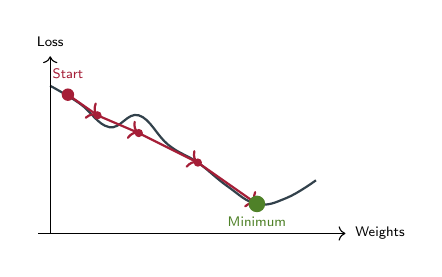
\begin{tikzpicture}[scale=0.75]
                % Loss landscape
                \draw[thick, TuebingenAnthrazit] plot[smooth, tension=0.7] coordinates {
                    (0, 2.5) (0.5, 2.2) (1, 1.8) (1.5, 2) (2, 1.5) (2.5, 1.2) (3, 0.8) (3.5, 0.5) (4, 0.6) (4.5, 0.9)
                };
                
                % Gradient descent path
                \fill[TuebingenRot] (0.3, 2.35) circle (3pt);
                \draw[->, TuebingenRot, thick] (0.3, 2.35) -- (0.8, 2);
                \fill[TuebingenRot] (0.8, 2) circle (2pt);
                \draw[->, TuebingenRot, thick] (0.8, 2) -- (1.5, 1.7);
                \fill[TuebingenRot] (1.5, 1.7) circle (2pt);
                \draw[->, TuebingenRot, thick] (1.5, 1.7) -- (2.5, 1.2);
                \fill[TuebingenRot] (2.5, 1.2) circle (2pt);
                \draw[->, TuebingenRot, thick] (2.5, 1.2) -- (3.5, 0.5);
                \fill[TuebingenGreen] (3.5, 0.5) circle (4pt);
                
                % Axes
                \draw[->] (-0.2, 0) -- (5, 0) node[right, font=\tiny] {Weights};
                \draw[->] (0, 0) -- (0, 3) node[above, font=\tiny] {Loss};
                
                % Labels
                \node[font=\tiny, TuebingenRot] at (0.3, 2.7) {Start};
                \node[font=\tiny, TuebingenGreen] at (3.5, 0.2) {Minimum};
            \end{tikzpicture}
        \end{center}
        {\small\centering Gradient descent: follow the slope downhill}
        
        \column{0.52\textwidth}
        \textbf{Gradient Descent} \cite{rumelhart1986backprop}:
        \begin{itemize}
            \setlength\itemsep{0.3em}
            \item Compute error (loss) on batch of data
            \item Calculate gradient: which direction reduces loss?
            \item Update weights: small step in that direction
            \item Repeat millions of times
        \end{itemize}
        
        \vspace{0.3em}
        \textbf{Key Hyperparameters:}
        \begin{itemize}
            \setlength\itemsep{0.2em}
            \item \textbf{Learning rate:} Step size (too big = overshoot, too small = slow)
            \item \textbf{Batch size:} Samples per gradient update
            \item \textbf{Epochs:} Passes through full dataset
        \end{itemize}
    \end{columns}
\end{frame}

\begin{frame}{Overfitting vs Underfitting}
    \framesubtitle{The fundamental tradeoff in machine learning}
    
    \vspace{0.3em}
    \begin{columns}[T]
        \column{0.32\textwidth}
        \begin{center}
            {\Large \color{TuebingenCyan} \textbf{Underfitting}}\\[0.3em]
            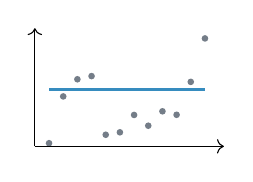
\begin{tikzpicture}[scale=0.6]
                \foreach \i in {1,...,12} {
                    \pgfmathsetmacro{\x}{0.3*\i}
                    \pgfmathsetmacro{\y}{0.5 + 0.3*\x + 0.8*rand}
                    \fill[TuebingenGray] (\x, \y) circle (2pt);
                }
                \draw[TuebingenCyan, very thick] (0.3, 1.2) -- (3.6, 1.2);
                \draw[->] (0,0) -- (4,0);
                \draw[->] (0,0) -- (0,2.5);
            \end{tikzpicture}
        \end{center}
        \begin{itemize}
            \setlength\itemsep{0.2em}
            \item Model too simple
            \item Misses patterns in data
            \item High error on \textit{both} train \& test
        \end{itemize}
        {\scriptsize\color{TuebingenGray} Fix: more capacity, features, training}
        
        \column{0.32\textwidth}
        \begin{center}
            {\Large \color{TuebingenGreen} \textbf{Good Fit}}\\[0.3em]
            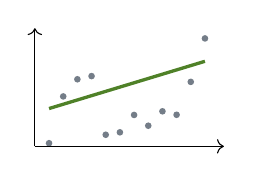
\begin{tikzpicture}[scale=0.6]
                \foreach \i in {1,...,12} {
                    \pgfmathsetmacro{\x}{0.3*\i}
                    \pgfmathsetmacro{\y}{0.5 + 0.3*\x + 0.8*rand}
                    \fill[TuebingenGray] (\x, \y) circle (2pt);
                }
                \draw[TuebingenGreen, very thick] (0.3, 0.8) -- (3.6, 1.8);
                \draw[->] (0,0) -- (4,0);
                \draw[->] (0,0) -- (0,2.5);
            \end{tikzpicture}
        \end{center}
        \begin{itemize}
            \setlength\itemsep{0.2em}
            \item Captures true pattern
            \item Ignores noise
            \item Generalizes to new data
        \end{itemize}
        {\scriptsize\color{TuebingenGreen} Goal: this is what we want}
        
        \column{0.32\textwidth}
        \begin{center}
            {\Large \color{TuebingenRot} \textbf{Overfitting}}\\[0.3em]
            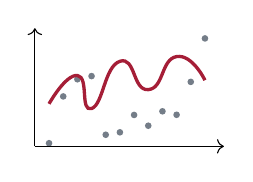
\begin{tikzpicture}[scale=0.6]
                \foreach \i in {1,...,12} {
                    \pgfmathsetmacro{\x}{0.3*\i}
                    \pgfmathsetmacro{\y}{0.5 + 0.3*\x + 0.8*rand}
                    \fill[TuebingenGray] (\x, \y) circle (2pt);
                }
                \draw[TuebingenRot, very thick] plot[smooth, tension=1] coordinates {
                    (0.3, 0.9) (0.9, 1.5) (1.2, 0.8) (1.8, 1.8) (2.4, 1.2) (3, 1.9) (3.6, 1.4)
                };
                \draw[->] (0,0) -- (4,0);
                \draw[->] (0,0) -- (0,2.5);
            \end{tikzpicture}
        \end{center}
        \begin{itemize}
            \setlength\itemsep{0.2em}
            \item Model memorizes training data
            \item Fits noise, not signal
            \item Fails on new data
        \end{itemize}
        {\scriptsize\color{TuebingenRot} The silent killer of ML projects}
    \end{columns}
    
    \vspace{0.3em}
    \begin{center}
        \small\color{TuebingenRot} \textbf{Executive insight:} A model that looks perfect on training data may be worthless in production. Always evaluate on held-out test data.
    \end{center}
\end{frame}

\begin{frame}{ML Failure Modes: Data Issues}
    \framesubtitle{The silent killers of AI projects}
    
    \vspace{0.3em}
    \begin{columns}[T]
        \column{0.48\textwidth}
        {\color{TuebingenRot}\textbf{Data Leakage}}
        
        \vspace{0.3em}
        Information from future/test leaks into training.
        
        \vspace{0.3em}
        \textbf{Symptoms:}
        \begin{itemize}
            \setlength\itemsep{0.3em}
            \item Model appears perfect in development
            \item Fails catastrophically in production
            \item "Too good to be true" metrics
        \end{itemize}
        
        \vspace{0.3em}
        \textbf{Common Examples:}
        \begin{itemize}
            \setlength\itemsep{0.3em}
            \item Using outcome data as input feature
            \item Time-series split done wrong
            \item Same customer in train and test
        \end{itemize}
        
        \column{0.48\textwidth}
        {\color{TuebingenGold}\textbf{Distribution Shift}}
        
        \vspace{0.3em}
        Production data differs from training data.
        
        \vspace{0.3em}
        \textbf{Symptoms:}
        \begin{itemize}
            \setlength\itemsep{0.3em}
            \item Model degrades over time
            \item Performance varies by segment
            \item Sudden accuracy drops
        \end{itemize}
        
        \vspace{0.3em}
        \textbf{Common Causes:}
        \begin{itemize}
            \setlength\itemsep{0.3em}
            \item Seasonality not captured
            \item Market changes post-training
            \item New user segments emerge
        \end{itemize}
    \end{columns}
    
    \vspace{0.5em}
    \begin{center}
        \small\color{TuebingenRot} \textbf{Executive insight:} These two issues cause most production ML failures.
    \end{center}
\end{frame}

\begin{frame}{ML Failure Modes: Label Quality}
    \framesubtitle{How we deceive ourselves about model quality}
    
    \vspace{0.5em}
    {\color{TuebingenCyan}\textbf{Label Quality Issues}} — Garbage in = garbage out.
    
    \vspace{0.5em}
    \textbf{Common Problems:}
    \begin{itemize}
        \setlength\itemsep{0.5em}
        \item Inconsistent labeling across annotators
        \item Missing labels for important cases
        \item Delayed labels (outcome not yet known)
        \item Label definitions change over time
    \end{itemize}
    
    \vspace{0.5em}
    {\color{TuebingenGray}\textbf{Reality:} Data quality work is often 80\% of ML effort.}
\end{frame}

\begin{frame}{ML Failure Modes: Evaluation Leakage}
    \framesubtitle{Overfitting to your test set}
    
    \vspace{0.5em}
    {\color{TuebingenGreen}\textbf{Evaluation Leakage}} — Overfitting to your test set.
    
    \vspace{0.5em}
    \textbf{Common Problems:}
    \begin{itemize}
        \setlength\itemsep{0.5em}
        \item Test set used repeatedly for tuning
        \item Overfitting to evaluation benchmark
        \item "Teaching to the test"
        \item Optimistic performance estimates
    \end{itemize}
    
    \vspace{0.5em}
    {\color{TuebingenGray}\textbf{Reality:} Each test set use reduces its validity.}
    
    \vspace{0.3em}
    \begin{theorembox}{Governance Requirement}
        Mandate \textbf{evaluation governance}: separate teams for model development and final evaluation, strict hold-out sets, documented data lineage, and drift monitoring.
    \end{theorembox}
\end{frame}

% ==============================================================================
% PART II-C: TRANSFORMERS, EMBEDDINGS, CONTEXT WINDOWS (25 minutes)
% ==============================================================================

% ------------------------------------------------------------------------------
% II-C.1 Embeddings: what they are and why they matter (3 slides + example)
% ------------------------------------------------------------------------------

\begin{frame}{Embeddings: The Foundation of Modern AI}
    \framesubtitle{Mapping discrete objects to meaningful vectors}
    
    {\color{TuebingenGray} An embedding maps discrete items (words, products, users) to vectors where \textit{geometry encodes meaning}.}
    
    \vspace{0.3em}
    \begin{columns}[T]
        \column{0.48\textwidth}
        \textbf{The Core Idea:}
        \begin{itemize}
            \setlength\itemsep{0.3em}
            \item Words/items → vectors of numbers
            \item Similar items → nearby vectors
            \item Relationships preserved geometrically
            \item Enables math on concepts
        \end{itemize}
        
        \vspace{0.2em}
        \textbf{Classic Example} \cite{mikolov2013word2vec}:
        \begin{center}
            \small
            $\vec{\text{king}} - \vec{\text{man}} + \vec{\text{woman}} \approx \vec{\text{queen}}$
        \end{center}
        {\scriptsize\color{TuebingenGray} Vector arithmetic captures semantic relationships}
        
        \column{0.48\textwidth}
        \begin{center}
            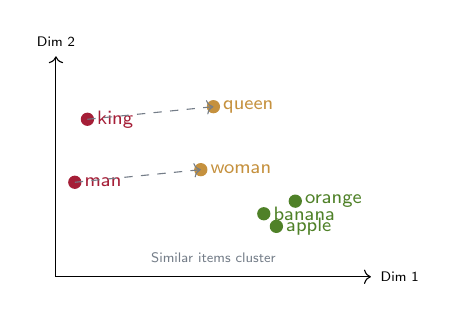
\begin{tikzpicture}[scale=0.8]
                % 2D embedding space visualization
                \fill[TuebingenRot] (0.5, 2.5) circle (3pt) node[right, font=\scriptsize] {king};
                \fill[TuebingenRot] (0.3, 1.5) circle (3pt) node[right, font=\scriptsize] {man};
                \fill[TuebingenGold] (2.5, 2.7) circle (3pt) node[right, font=\scriptsize] {queen};
                \fill[TuebingenGold] (2.3, 1.7) circle (3pt) node[right, font=\scriptsize] {woman};
                
                % Relationship arrows
                \draw[->, TuebingenGray, dashed] (0.5, 2.5) -- (2.5, 2.7);
                \draw[->, TuebingenGray, dashed] (0.3, 1.5) -- (2.3, 1.7);
                
                % More words
                \fill[TuebingenGreen] (3.5, 0.8) circle (3pt) node[right, font=\scriptsize] {apple};
                \fill[TuebingenGreen] (3.8, 1.2) circle (3pt) node[right, font=\scriptsize] {orange};
                \fill[TuebingenGreen] (3.3, 1.0) circle (3pt) node[right, font=\scriptsize] {banana};
                
                % Axes
                \draw[->] (0,0) -- (5,0) node[right, font=\tiny] {Dim 1};
                \draw[->] (0,0) -- (0,3.5) node[above, font=\tiny] {Dim 2};
                
                % Annotation
                \node[font=\tiny, TuebingenGray] at (2.5, 0.3) {Similar items cluster};
            \end{tikzpicture}
        \end{center}
    \end{columns}
\end{frame}

\begin{frame}{What Can Be Embedded?}
    \framesubtitle{Embeddings work for almost any discrete data}
    
    \vspace{0.3em}
    \begin{columns}[T]
        \column{0.48\textwidth}
        \textbf{Text Embeddings:}
        \begin{itemize}
            \setlength\itemsep{0.3em}
            \item Words, sentences, documents
            \item Enable semantic search
            \item Power RAG systems
            \item Compare meaning, not keywords
        \end{itemize}
        
        \vspace{0.3em}
        \textbf{Image Embeddings:}
        \begin{itemize}
            \setlength\itemsep{0.3em}
            \item Images → vectors via CNN/ViT
            \item Visual similarity search
            \item Reverse image search
            \item Content moderation
        \end{itemize}
        
        \column{0.48\textwidth}
        \textbf{User/Product Embeddings:}
        \begin{itemize}
            \setlength\itemsep{0.3em}
            \item Collaborative filtering
            \item "Users like you bought..."
            \item Personalized recommendations
        \end{itemize}
        
        \vspace{0.3em}
        \textbf{Code Embeddings:}
        \begin{itemize}
            \setlength\itemsep{0.3em}
            \item Functions → vectors
            \item Find similar code
            \item Semantic code search
            \item Duplicate detection
        \end{itemize}
    \end{columns}
    
    \vspace{0.5em}
    \begin{center}
        \small\color{TuebingenRot} \textbf{Key insight:} Embeddings are the universal interface. Text, images, users, products—all become vectors that can be compared, clustered, and retrieved.
    \end{center}
\end{frame}

\begin{frame}{Embeddings Example: Semantic Search}
    \framesubtitle{Finding relevant documents by meaning, not keywords}
    
    \vspace{0.3em}
    \begin{columns}[T]
        \column{0.48\textwidth}
        \textbf{Traditional Keyword Search:}
        \begin{itemize}
            \setlength\itemsep{0.3em}
            \item Query: "vacation policy"
            \item Matches: documents containing "vacation" AND "policy"
            \item \textcolor{TuebingenRot}{Misses:} "PTO guidelines", "time off procedures", "leave entitlement"
        \end{itemize}
        
        \vspace{0.3em}
        \textbf{Semantic Search with Embeddings:}
        \begin{itemize}
            \setlength\itemsep{0.3em}
            \item Query → embedding vector
            \item Find documents with similar vectors
            \item \textcolor{TuebingenGreen}{Finds:} All semantically related docs, regardless of exact wording
        \end{itemize}
        
        \column{0.48\textwidth}
        \begin{center}
            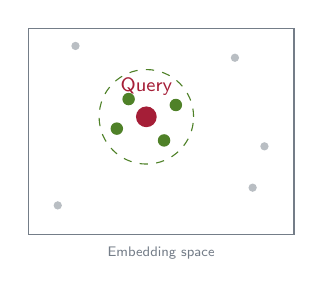
\begin{tikzpicture}[scale=0.75]
                % Query point
                \fill[TuebingenRot] (2, 2) circle (5pt);
                \node[font=\scriptsize, TuebingenRot, above] at (2, 2.2) {Query};
                
                % Relevant docs (nearby)
                \fill[TuebingenGreen] (2.3, 1.6) circle (3pt);
                \fill[TuebingenGreen] (1.7, 2.3) circle (3pt);
                \fill[TuebingenGreen] (2.5, 2.2) circle (3pt);
                \fill[TuebingenGreen] (1.5, 1.8) circle (3pt);
                
                % Circle showing retrieval radius
                \draw[TuebingenGreen, dashed] (2, 2) circle (0.8);
                
                % Irrelevant docs (far)
                \fill[TuebingenGray!50] (0.5, 0.5) circle (2pt);
                \fill[TuebingenGray!50] (3.8, 0.8) circle (2pt);
                \fill[TuebingenGray!50] (0.8, 3.2) circle (2pt);
                \fill[TuebingenGray!50] (3.5, 3) circle (2pt);
                \fill[TuebingenGray!50] (4, 1.5) circle (2pt);
                
                % Frame
                \draw[TuebingenGray] (0,0) rectangle (4.5, 3.5);
                \node[font=\tiny, TuebingenGray] at (2.25, -0.3) {Embedding space};
            \end{tikzpicture}
        \end{center}
        
        {\small\color{TuebingenGray} Retrieve $k$ nearest neighbors}
    \end{columns}
\end{frame}

\begin{frame}{Enterprise Value}
    \vspace{0.3em}
    \begin{theorembox}{Enterprise Value}
        Embedding-based search is the backbone of \textbf{RAG systems}. \\
        It enables AI assistants to find relevant internal documents even when users don't know the exact terminology.
    \end{theorembox}
\end{frame}

% ------------------------------------------------------------------------------
% II-C.2 Transformer architecture: the minimal correct explanation (4 slides)
% ------------------------------------------------------------------------------

\begin{frame}{Transformers: The Architecture Behind LLMs}
    \framesubtitle{Why "Attention Is All You Need"}
    
    {\color{TuebingenGray} The Transformer architecture \cite{vaswani2017attention} revolutionized NLP and enabled today's large language models.}
    
    \vspace{0.2em}
    \begin{columns}[T]
        \column{0.48\textwidth}
        \textbf{Before Transformers (RNNs/LSTMs):}
        \begin{itemize}
            \setlength\itemsep{0.2em}
            \item Process text \textit{sequentially}, word by word
            \item Hard to parallelize → slow training
            \item Long-range dependencies get "forgotten"
            \item Limited context window
        \end{itemize}
        
        \vspace{0.2em}
        \textbf{The Transformer Innovation:}
        \begin{itemize}
            \setlength\itemsep{0.2em}
            \item Process all tokens \textit{in parallel}
            \item \textbf{Attention:} Each token can "look at" all others
            \item No sequential bottleneck
            \item Scales to massive models
        \end{itemize}
        
        \column{0.48\textwidth}
        \begin{center}
            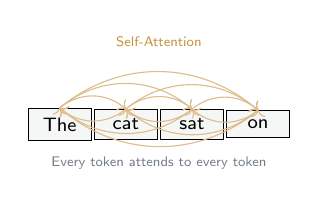
\begin{tikzpicture}[scale=0.7]
                % Tokens
                \node[draw, fill=TuebingenBeige, minimum width=0.8cm, font=\scriptsize] (t1) at (0, 0) {The};
                \node[draw, fill=TuebingenBeige, minimum width=0.8cm, font=\scriptsize] (t2) at (1.2, 0) {cat};
                \node[draw, fill=TuebingenBeige, minimum width=0.8cm, font=\scriptsize] (t3) at (2.4, 0) {sat};
                \node[draw, fill=TuebingenBeige, minimum width=0.8cm, font=\scriptsize] (t4) at (3.6, 0) {on};
                
                % Attention arrows (all-to-all)
                \foreach \i in {t1, t2, t3, t4} {
                    \foreach \j in {t1, t2, t3, t4} {
                        \draw[->, TuebingenGold!60, thin] (\i.north) to[bend left=40] (\j.north);
                    }
                }
                
                % Label
                \node[font=\tiny, TuebingenGold] at (1.8, 1.5) {Self-Attention};
                \node[font=\tiny, TuebingenGray] at (1.8, -0.7) {Every token attends to every token};
            \end{tikzpicture}
        \end{center}
    \end{columns}
    
    \vspace{0.3em}
    \begin{center}
        \small\color{TuebingenGreen} \textbf{Result:} Training that took weeks now takes hours. Models can be 1000× larger.
    \end{center}
\end{frame}

\begin{frame}{The Attention Mechanism}
    \framesubtitle{Content-addressable retrieval within the input}
    
    {\color{TuebingenGray} Attention lets the model dynamically decide which parts of the input are relevant to each output.}
    
    \vspace{0.3em}
    \begin{columns}[T]
        \column{0.50\textwidth}
        \textbf{Intuition:}
        \begin{itemize}
            \setlength\itemsep{0.3em}
            \item For each token, ask: "What should I pay attention to?"
            \item Compute relevance scores to all other tokens
            \item Weight information by relevance
            \item Aggregate: weighted sum of values
        \end{itemize}
        
        \vspace{0.2em}
        \textbf{The Q-K-V Framework:}
        \begin{itemize}
            \setlength\itemsep{0.2em}
            \item \textbf{Query (Q):} "What am I looking for?"
            \item \textbf{Key (K):} "What do I contain?"
            \item \textbf{Value (V):} "What information do I provide?"
            \item Score = Query · Key (dot product)
        \end{itemize}
        
        \column{0.47\textwidth}
        \textbf{Example — Resolving "it":}
        
        \vspace{0.2em}
        {\small "The \textcolor{TuebingenGold}{cat} sat on the mat because \textcolor{TuebingenRot}{it} was tired."}
        
        \vspace{0.3em}
        \begin{center}
            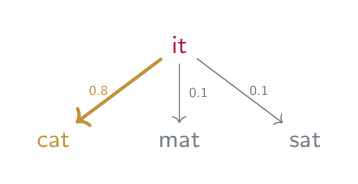
\begin{tikzpicture}[scale=0.8]
                \node[font=\small, TuebingenRot] (it) at (2, 2) {it};
                \node[font=\small, TuebingenGold] (cat) at (0, 0.5) {cat};
                \node[font=\small, TuebingenGray] (mat) at (2, 0.5) {mat};
                \node[font=\small, TuebingenGray] (sat) at (4, 0.5) {sat};
                
                % Attention weights
                \draw[->, very thick, TuebingenGold] (it) -- (cat) node[midway, left, font=\tiny] {0.8};
                \draw[->, thin, TuebingenGray] (it) -- (mat) node[midway, right, font=\tiny] {0.1};
                \draw[->, thin, TuebingenGray] (it) -- (sat) node[midway, right, font=\tiny] {0.1};
            \end{tikzpicture}
        \end{center}
        
        {\small\color{TuebingenGray} Attention learns that "it" refers to "cat" with high probability}
    \end{columns}
\end{frame}

\begin{frame}{Transformer Variants: Encoder, Decoder, and Both}
    \framesubtitle{Different architectures for different tasks}
    
    \vspace{0.3em}
    \begin{columns}[T]
        \column{0.32\textwidth}
        \begin{center}
            {\color{TuebingenRot}\textbf{Encoder-Only}}\\[0.2em]
            {\small (BERT-style)} \cite{devlin2019bert}
        \end{center}
        \vspace{0.3em}
        \begin{itemize}
            \setlength\itemsep{0.2em}
            \item Bidirectional attention
            \item Sees full input at once
            \item Best for: understanding
        \end{itemize}
        \vspace{0.3em}
        {\scriptsize\color{TuebingenGray} 
            \textbf{Tasks:} Classification, NER, embeddings, similarity
        }
        
        \column{0.32\textwidth}
        \begin{center}
            {\color{TuebingenGold}\textbf{Decoder-Only}}\\[0.2em]
            {\small (GPT-style)} \cite{brown2020gpt3}
        \end{center}
        \vspace{0.3em}
        \begin{itemize}
            \setlength\itemsep{0.2em}
            \item Causal attention (left-to-right)
            \item Generates token by token
            \item Best for: generation
        \end{itemize}
        \vspace{0.3em}
        {\scriptsize\color{TuebingenGray} 
            \textbf{Tasks:} Text generation, chat, code, reasoning
        }
        
        \column{0.32\textwidth}
        \begin{center}
            {\color{TuebingenGreen}\textbf{Encoder-Decoder}}\\[0.2em]
            {\small (T5-style)}
        \end{center}
        \vspace{0.3em}
        \begin{itemize}
            \setlength\itemsep{0.2em}
            \item Encoder reads input
            \item Decoder generates output
            \item Best for: transformation
        \end{itemize}
        \vspace{0.3em}
        {\scriptsize\color{TuebingenGray} 
            \textbf{Tasks:} Translation, summarization, Q\&A
        }
    \end{columns}
    
    \vspace{0.3em}
    \begin{theorembox}{What You're Using Today}
        ChatGPT, Claude, Gemini, Llama = \textbf{Decoder-only} transformers \\
        They generate text left-to-right, predicting the next token given all previous tokens.
    \end{theorembox}
\end{frame}

\begin{frame}{How LLMs Generate Text}
    \framesubtitle{From prompt to completion}
    
    {\color{TuebingenGray} Text generation is iterative: predict next token, append, repeat.}
    
    \vspace{0.3em}
    \begin{columns}[T]
        \column{0.55\textwidth}
        \textbf{The Generation Loop:}
        \begin{enumerate}
            \setlength\itemsep{0.3em}
            \item \textbf{Encode prompt} into token IDs
            \item \textbf{Forward pass}: compute probability distribution over vocabulary
            \item \textbf{Sample} next token (with temperature)
            \item \textbf{Append} token to sequence
            \item \textbf{Repeat} until stop token or max length
        \end{enumerate}
        
        \vspace{0.3em}
        \textbf{Temperature Controls Randomness:}
        \begin{itemize}
            \setlength\itemsep{0.2em}
            \item $T \rightarrow 0$: Always pick most likely (deterministic)
            \item $T = 1$: Sample from learned distribution
            \item $T > 1$: More random/creative
        \end{itemize}
        
        \column{0.42\textwidth}
        \begin{center}
            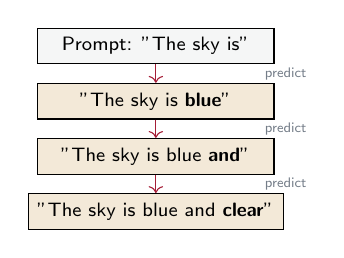
\begin{tikzpicture}[scale=0.7]
                % Steps
                \node[draw, fill=TuebingenBeige, font=\scriptsize, minimum width=3cm] (p) at (0, 3) {Prompt: "The sky is"};
                
                \node[draw, fill=TuebingenGold!20, font=\scriptsize, minimum width=3cm] (s1) at (0, 2) {"The sky is \textbf{blue}"};
                
                \node[draw, fill=TuebingenGold!20, font=\scriptsize, minimum width=3cm] (s2) at (0, 1) {"The sky is blue \textbf{and}"};
                
                \node[draw, fill=TuebingenGold!20, font=\scriptsize, minimum width=3cm] (s3) at (0, 0) {"The sky is blue and \textbf{clear}"};
                
                % Arrows
                \draw[->, TuebingenRot] (p) -- (s1);
                \draw[->, TuebingenRot] (s1) -- (s2);
                \draw[->, TuebingenRot] (s2) -- (s3);
                
                % Labels
                \node[font=\tiny, TuebingenGray, right] at (1.8, 2.5) {predict};
                \node[font=\tiny, TuebingenGray, right] at (1.8, 1.5) {predict};
                \node[font=\tiny, TuebingenGray, right] at (1.8, 0.5) {predict};
            \end{tikzpicture}
        \end{center}
    \end{columns}
    
    \vspace{0.3em}
    \begin{center}
        \small\color{TuebingenRot} \textbf{Key insight:} LLMs don't "understand"—they predict statistically likely continuations based on training data patterns.
    \end{center}
\end{frame}

% ------------------------------------------------------------------------------
% II-C.3 Context windows: capability, cost, and risk (2 slides + example)
% ------------------------------------------------------------------------------

\begin{frame}{Context Windows: The Memory Limit}
    \framesubtitle{What the model can "see" at once}
    
    {\color{TuebingenGray} The context window is the maximum number of tokens (prompt + response) the model can process.}
    
    \vspace{0.3em}
    \begin{columns}[T]
        \column{0.48\textwidth}
        \textbf{Context Window Evolution:}
        \begin{itemize}
            \setlength\itemsep{0.2em}
            \item GPT-3 (2020): 4K tokens
            \item GPT-4 (2023): 8K–128K tokens
            \item Claude 3 (2024): 200K tokens
            \item Gemini 1.5 (2024): 1M+ tokens
        \end{itemize}
        
        \vspace{0.3em}
        \textbf{What's a Token?}
        \begin{itemize}
            \setlength\itemsep{0.2em}
            \item Roughly 0.75 words in English
            \item 4K tokens ≈ 3,000 words ≈ 6 pages
            \item 128K tokens ≈ a short book
        \end{itemize}
        
        \column{0.48\textwidth}
        \textbf{Why It Matters:}
        \begin{itemize}
            \setlength\itemsep{0.3em}
            \item Larger context = more information available
            \item Can include more documents, longer conversations
            \item \textcolor{TuebingenRot}{But:} Compute and cost scale with context
        \end{itemize}
        
        \vspace{0.2em}
        \textbf{The Trade-offs:}
        \begin{itemize}
            \setlength\itemsep{0.2em}
            \item \textbf{Cost:} Proportional to tokens processed
            \item \textbf{Latency:} Longer context = slower response
            \item \textbf{Quality:} "Lost in the middle" problem
        \end{itemize}
    \end{columns}
\end{frame}

\begin{frame}{Context Window Strategy: Less Is Often More}
    \framesubtitle{Smart retrieval beats context stuffing}
    
    \vspace{0.2em}
    \begin{columns}[T]
        \column{0.48\textwidth}
        {\color{TuebingenRot}\textbf{Naive Approach:}}\\[0.2em]
        "Dump everything into context"
        \begin{itemize}
            \setlength\itemsep{0.2em}
            \item Include all potentially relevant docs
            \item Max out the context window
            \item Let the model figure it out
        \end{itemize}
        
        \vspace{0.2em}
        \textbf{Problems:}
        \begin{itemize}
            \setlength\itemsep{0.15em}
            \item High cost (pay per token)
            \item Slower responses
            \item Model gets distracted by irrelevant info
            \item "Lost in the middle" — info in middle gets ignored
        \end{itemize}
        
        \column{0.48\textwidth}
        {\color{TuebingenGreen}\textbf{Smart Approach:}}\\[0.2em]
        "Retrieve only what's relevant"
        \begin{itemize}
            \setlength\itemsep{0.2em}
            \item Use embeddings to find relevant passages
            \item Include only top-$k$ most relevant
            \item Keep context focused and concise
        \end{itemize}
        
        \vspace{0.2em}
        \textbf{Benefits:}
        \begin{itemize}
            \setlength\itemsep{0.15em}
            \item Lower cost
            \item Faster responses
            \item Better answer quality
            \item Clearer citation/attribution
        \end{itemize}
    \end{columns}
\end{frame}

\begin{frame}{RAG: Design Principle}
    \vspace{0.3em}
    \begin{theorembox}{Design Principle}
        \textbf{RAG + small context} often outperforms \textbf{no RAG + huge context}. \\
        Relevance filtering is not just cost optimization—it improves quality.
    \end{theorembox}
\end{frame}

% ------------------------------------------------------------------------------
% II-C.4 Tool use and agentic patterns (optional 2 slides)
% ------------------------------------------------------------------------------

\begin{frame}{Tool Use: Extending LLM Capabilities}
    \framesubtitle{When generation isn't enough}
    
    {\color{TuebingenGray} LLMs can call external tools—calculators, APIs, databases—to overcome their limitations.}
    
    \vspace{0.5em}
    \textbf{Why Tool Use?}
    \begin{itemize}
        \setlength\itemsep{0.4em}
        \item LLMs are bad at math → \textbf{call calculator}
        \item LLMs have stale knowledge → \textbf{call search API}
        \item LLMs can't access your data → \textbf{call database}
        \item LLMs can't take actions → \textbf{call business APIs}
    \end{itemize}
    
    \vspace{0.5em}
    \textbf{How It Works:}
    \begin{enumerate}
        \setlength\itemsep{0.4em}
        \item Model outputs structured tool call
        \item System executes tool, returns result
        \item Model continues with result in context
    \end{enumerate}
\end{frame}

\begin{frame}{Tool Use: Example Flow}
    \framesubtitle{Database query example}
    
    \vspace{0.5em}
    \textbf{Example Flow:}
    \begin{enumerate}
        \setlength\itemsep{0.5em}
        \item User: "What's our Q3 revenue?"
        \item Model decides: \texttt{query\_database("Q3 revenue")}
        \item System executes query → returns "\$4.2M"
        \item Model responds: "Your Q3 revenue was \$4.2M"
    \end{enumerate}
    
    \vspace{0.5em}
    \textbf{Common Tools:}
    \begin{itemize}
        \setlength\itemsep{0.4em}
        \item Code execution (Python interpreter)
        \item Web search
        \item Database queries
        \item API calls (CRM, ERP, etc.)
    \end{itemize}
\end{frame}

\begin{frame}{Agentic Patterns: What Makes an Agent}
    \framesubtitle{Multi-step reasoning with tools}
    
    {\color{TuebingenGray} Agents combine LLMs + tools + planning to accomplish complex tasks autonomously.}
    
    \vspace{0.5em}
    \begin{columns}[T]
        \column{0.48\textwidth}
        \textbf{Core Components:}
        \begin{itemize}
            \setlength\itemsep{0.5em}
            \item \textbf{Planning:} Break task into steps
            \item \textbf{Tool use:} Execute actions
            \item \textbf{Memory:} Track progress and context
            \item \textbf{Reflection:} Evaluate and adjust
        \end{itemize}
        
        \column{0.48\textwidth}
        \textbf{Example — Research Agent:}
        \begin{enumerate}
            \setlength\itemsep{0.4em}
            \item Plan: "Need 3 competitor analyses"
            \item Search: Query web for each competitor
            \item Analyze: Extract key info
            \item Synthesize: Compile report
            \item Reflect: "Is this complete?"
        \end{enumerate}
    \end{columns}
    
    \vspace{0.5em}
    \begin{center}
        {\color{TuebingenGold}\textbf{Key insight:} Agents are LLMs that can take actions, not just generate text.}
    \end{center}
\end{frame}

\begin{frame}{Agentic Patterns: Governance Requirements}
    \framesubtitle{Bounded autonomy with guardrails}
    
    \vspace{0.5em}
    {\color{TuebingenRot}\textbf{What Must Be Controlled:}}
    
    \vspace{0.3em}
    \begin{columns}[T]
        \column{0.48\textwidth}
        \begin{itemize}
            \setlength\itemsep{0.5em}
            \item \textbf{Permissions:} What can the agent access?
            \item \textbf{Audit:} Log all tool calls and decisions
            \item \textbf{Limits:} Max steps, cost caps, time bounds
        \end{itemize}
        
        \column{0.48\textwidth}
        \begin{itemize}
            \setlength\itemsep{0.5em}
            \item \textbf{Human-in-loop:} Approval for sensitive actions
            \item \textbf{Fail-safes:} What if agent goes off-track?
            \item \textbf{Rollback:} Undo harmful actions
        \end{itemize}
    \end{columns}
    
    \vspace{0.5em}
    \begin{theorembox}{Executive Caution}
        Agentic systems are powerful but harder to control. \\
        Start with \textbf{narrow, well-defined tasks} and \textbf{explicit guardrails}. \\
        Expand autonomy gradually as you build trust and monitoring capability.
    \end{theorembox}
\end{frame}

% ==============================================================================
% PART II-D: RAG SYSTEMS IN DETAIL (25 minutes)
% ==============================================================================

\begin{frame}{Part II-D: RAG Systems in Detail}
    \framesubtitle{25 minutes — The primary lever for enterprise value}
    
    \vspace{0.5em}
    \begin{center}
        {\Large\color{TuebingenRot} Retrieval-Augmented Generation}
        
        \vspace{0.3em}
        {\color{TuebingenGray} The architecture pattern that makes LLMs useful for enterprise knowledge}
    \end{center}
    
    \vspace{0.5em}
    \begin{theorembox}{Why This Matters}
        RAG is how enterprises get \textbf{accurate, grounded, auditable} answers \\
        from LLMs about their \textbf{own} data. Get this right → unlock value. Get it wrong → liability.
    \end{theorembox}
    
    \vspace{0.5em}
    \begin{center}
        {\small\color{TuebingenGray} We'll start with the AI building blocks, then assemble the full pipeline.}
    \end{center}
\end{frame}

% ------------------------------------------------------------------------------
% II-D.0 RAG Prerequisites: The AI Building Blocks
% ------------------------------------------------------------------------------

\begin{frame}{RAG: The AI Building Blocks}
    \framesubtitle{Three technologies that make RAG possible}
    
    \vspace{0.3em}
    \begin{center}
        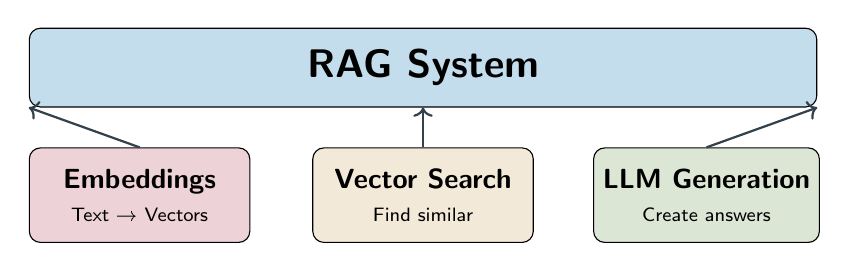
\begin{tikzpicture}[scale=0.9]
            % Three pillars
            \node[draw, fill=TuebingenRot!20, rounded corners, minimum width=2.8cm, minimum height=1.2cm, align=center] (embed) at (0,0) {\textbf{Embeddings}\\{\scriptsize Text → Vectors}};
            \node[draw, fill=TuebingenGold!20, rounded corners, minimum width=2.8cm, minimum height=1.2cm, align=center] (vector) at (4,0) {\textbf{Vector Search}\\{\scriptsize Find similar}};
            \node[draw, fill=TuebingenGreen!20, rounded corners, minimum width=2.8cm, minimum height=1.2cm, align=center] (llm) at (8,0) {\textbf{LLM Generation}\\{\scriptsize Create answers}};
            
            % RAG on top
            \node[draw, fill=TuebingenCyan!30, rounded corners, minimum width=10cm, minimum height=1cm, align=center] (rag) at (4,1.8) {\Large\textbf{RAG System}};
            
            % Arrows
            \draw[->, thick, TuebingenAnthrazit] (embed.north) -- (rag.south west);
            \draw[->, thick, TuebingenAnthrazit] (vector.north) -- (rag.south);
            \draw[->, thick, TuebingenAnthrazit] (llm.north) -- (rag.south east);
        \end{tikzpicture}
    \end{center}
    
    \vspace{0.5em}
    \begin{columns}[T]
        \column{0.32\textwidth}
        \begin{center}
            {\color{TuebingenRot}\textbf{1. Embeddings}}
        \end{center}
        Convert text into numerical vectors that capture meaning.
        
        \column{0.32\textwidth}
        \begin{center}
            {\color{TuebingenGold}\textbf{2. Vector Search}}
        \end{center}
        Find documents similar to a query based on vector distance.
        
        \column{0.32\textwidth}
        \begin{center}
            {\color{TuebingenGreen}\textbf{3. LLM Generation}}
        \end{center}
        Synthesize an answer from retrieved context.
    \end{columns}
    
    \vspace{0.5em}
    \begin{center}
        \small\color{TuebingenGray} Let's understand each building block before assembling them.
    \end{center}
\end{frame}

\begin{frame}{Building Block 1: Embeddings}
    \framesubtitle{Turning text into numbers that capture meaning}
    
    \vspace{0.3em}
    \begin{columns}[T]
        \column{0.48\textwidth}
        \textbf{What is an Embedding?}
        \begin{itemize}
            \setlength\itemsep{0.4em}
            \item A \textbf{vector} (list of numbers) representing text
            \item Typical size: 384–1536 dimensions
            \item Created by a neural network trained on massive text
            \item \textbf{Key property:} Similar meaning → similar vectors
        \end{itemize}
        
        \vspace{0.3em}
        \textbf{Example:}
        \begin{itemize}
            \setlength\itemsep{0.3em}
            \item "vacation policy" → [0.23, -0.41, 0.87, ...]
            \item "time off guidelines" → [0.25, -0.38, 0.84, ...]
            \item "server configuration" → [-0.71, 0.12, -0.33, ...]
        \end{itemize}
        
        \column{0.48\textwidth}
        \begin{center}
            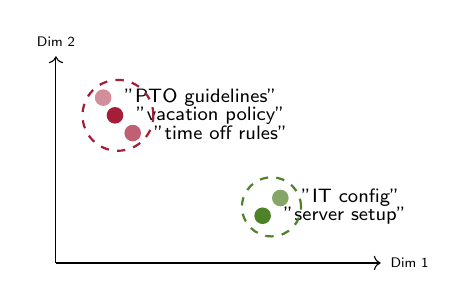
\begin{tikzpicture}[scale=0.75]
                % Embedding space visualization
                \fill[TuebingenRot] (1, 2.5) circle (4pt);
                \node[font=\scriptsize, right] at (1.2, 2.5) {"vacation policy"};
                
                \fill[TuebingenRot!70] (1.3, 2.2) circle (4pt);
                \node[font=\scriptsize, right] at (1.5, 2.2) {"time off rules"};
                
                \fill[TuebingenRot!50] (0.8, 2.8) circle (4pt);
                \node[font=\scriptsize, right] at (1, 2.8) {"PTO guidelines"};
                
                \fill[TuebingenGreen] (3.5, 0.8) circle (4pt);
                \node[font=\scriptsize, right] at (3.7, 0.8) {"server setup"};
                
                \fill[TuebingenGreen!70] (3.8, 1.1) circle (4pt);
                \node[font=\scriptsize, right] at (4, 1.1) {"IT config"};
                
                % Axes
                \draw[->] (0,0) -- (5.5,0) node[right, font=\tiny] {Dim 1};
                \draw[->] (0,0) -- (0,3.5) node[above, font=\tiny] {Dim 2};
                
                % Cluster indicators
                \draw[TuebingenRot, dashed, thick] (1.05, 2.5) circle (0.6);
                \draw[TuebingenGreen, dashed, thick] (3.65, 0.95) circle (0.5);
            \end{tikzpicture}
        \end{center}
        
        {\small\centering\color{TuebingenGray} Similar topics cluster together}
    \end{columns}
    
    \vspace{0.3em}
    \begin{center}
        \small\color{TuebingenRot} \textbf{Key insight:} Embeddings let us find documents by \textit{meaning}, not just keywords.
    \end{center}
\end{frame}

\begin{frame}{Building Block 2: Vector Search}
    \framesubtitle{Finding relevant documents by similarity}
    
    \vspace{0.3em}
    \begin{columns}[T]
        \column{0.48\textwidth}
        \textbf{How Vector Search Works:}
        \begin{enumerate}
            \setlength\itemsep{0.4em}
            \item \textbf{Index:} Store document embeddings in a vector database
            \item \textbf{Query:} Convert user question to embedding
            \item \textbf{Search:} Find k-nearest vectors (most similar documents)
            \item \textbf{Return:} Documents ranked by similarity
        \end{enumerate}
        
        \vspace{0.3em}
        \textbf{Similarity Measures:}
        \begin{itemize}
            \setlength\itemsep{0.2em}
            \item \textbf{Cosine similarity:} Angle between vectors
            \item \textbf{Euclidean distance:} Straight-line distance
            \item \textbf{Dot product:} For normalized vectors
        \end{itemize}
        
        \column{0.48\textwidth}
        \begin{center}
            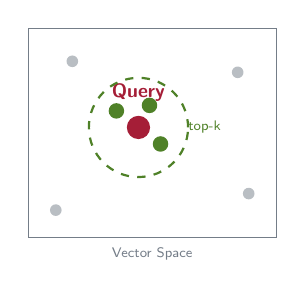
\begin{tikzpicture}[scale=0.7]
                % Query point
                \fill[TuebingenRot] (2, 2) circle (6pt);
                \node[font=\scriptsize, TuebingenRot, above] at (2, 2.3) {\textbf{Query}};
                
                % Document points
                \fill[TuebingenGreen] (2.4, 1.7) circle (4pt);
                \fill[TuebingenGreen] (1.6, 2.3) circle (4pt);
                \fill[TuebingenGreen] (2.2, 2.4) circle (4pt);
                
                \fill[TuebingenGray!50] (0.5, 0.5) circle (3pt);
                \fill[TuebingenGray!50] (4, 0.8) circle (3pt);
                \fill[TuebingenGray!50] (0.8, 3.2) circle (3pt);
                \fill[TuebingenGray!50] (3.8, 3) circle (3pt);
                
                % Search radius
                \draw[TuebingenGreen, dashed, thick] (2, 2) circle (0.9);
                \node[font=\tiny, TuebingenGreen] at (3.2, 2) {top-k};
                
                % Frame
                \draw[TuebingenGray] (0,0) rectangle (4.5, 3.8);
                \node[font=\tiny, TuebingenGray] at (2.25, -0.3) {Vector Space};
            \end{tikzpicture}
        \end{center}
        
        \vspace{0.2em}
        {\small\centering Green = retrieved documents}
    \end{columns}
    
\end{frame}

\begin{frame}{Building Block 3: LLM Generation}
    \framesubtitle{Synthesizing answers from context}
    
    \vspace{0.3em}
    \begin{columns}[T]
        \column{0.48\textwidth}
        \textbf{What the LLM Does in RAG:}
        \begin{itemize}
            \setlength\itemsep{0.4em}
            \item \textbf{Reads} retrieved documents as context
            \item \textbf{Understands} the user's question
            \item \textbf{Synthesizes} an answer from the context
            \item \textbf{Cites} which documents support claims
        \end{itemize}
        
        \vspace{0.3em}
        \textbf{The Prompt Structure:}
        \begin{enumerate}
            \setlength\itemsep{0.3em}
            \item System: "Answer based only on provided context"
            \item Context: [Retrieved documents]
            \item User: "What is our vacation policy?"
        \end{enumerate}
        
        \column{0.48\textwidth}
        \textbf{Why Not Just Use the LLM?}
        
        \vspace{0.3em}
        Without retrieved context:
        \begin{itemize}
            \setlength\itemsep{0.3em}
            \item {\color{TuebingenRot}\textbf{Hallucination:}} Makes up policies
            \item {\color{TuebingenRot}\textbf{Stale:}} Training cutoff date
            \item {\color{TuebingenRot}\textbf{Generic:}} No company-specific info
        \end{itemize}
        
        \vspace{0.3em}
        With retrieved context:
        \begin{itemize}
            \setlength\itemsep{0.3em}
            \item {\color{TuebingenGreen}\textbf{Grounded:}} Uses actual docs
            \item {\color{TuebingenGreen}\textbf{Current:}} Latest indexed version
            \item {\color{TuebingenGreen}\textbf{Citable:}} Can reference source
        \end{itemize}
    \end{columns}
    
    \vspace{0.3em}
    \begin{center}
        \small\color{TuebingenRot} \textbf{Key insight:} The LLM's job is to \textit{read and summarize}, not to \textit{remember}.
    \end{center}
\end{frame}

\begin{frame}{Putting It Together: The RAG Flow}
    \framesubtitle{How the three building blocks combine}
    
    % Increase vertical spacing for more slide coverage
    \vspace{0.8em}
    \begin{center}
        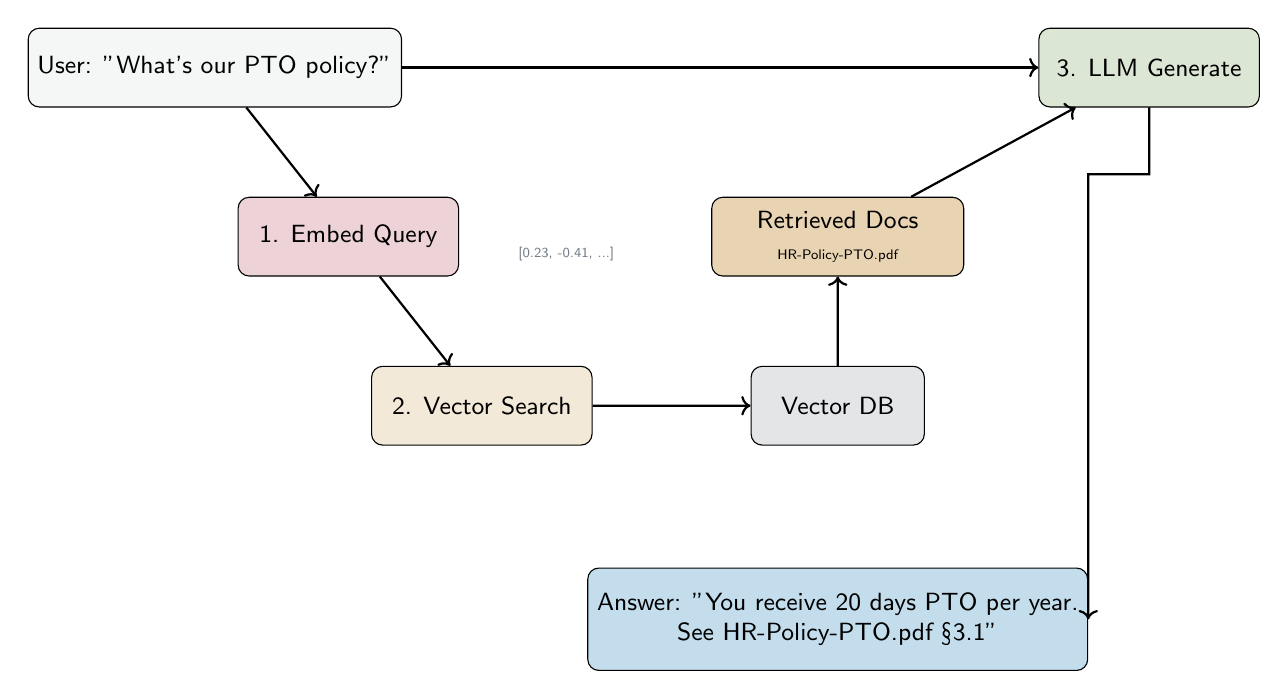
\begin{tikzpicture}[scale=1.13, every node/.style={font=\small}]
            % User query (far left, near top)
            \node[draw, fill=TuebingenBeige, rounded corners, minimum width=3.2cm, minimum height=1cm] (query) at (-5, 3.4) {User: "What's our PTO policy?"};
            
            % Step 1: Embed query (closer to left, a bit lower)
            \node[draw, fill=TuebingenRot!20, rounded corners, minimum width=2.8cm, minimum height=1cm] (embed) at (-3.5, 1.5) {1. Embed Query};
            \node[font=\tiny, TuebingenGray, right] at (-1.7, 1.3) {[0.23, -0.41, ...]};
            
            % Step 2: Vector search (center left)
            \node[draw, fill=TuebingenGold!20, rounded corners, minimum width=2.8cm, minimum height=1cm] (search) at (-2, -0.4) {2. Vector Search};
            
            % Vector DB (center right)
            \node[draw, fill=TuebingenGray!20, rounded corners, minimum width=2.2cm, minimum height=1cm] (db) at (2, -0.4) {Vector DB};
            
            % Step 3: Retrieved docs (center top)
            \node[draw, fill=TuebingenGold!40, rounded corners, minimum width=3.2cm, minimum height=1cm, align=center] (docs) at (2, 1.5) {Retrieved Docs\\{\tiny HR-Policy-PTO.pdf}};
            
            % Step 4: LLM (far right, top)
            \node[draw, fill=TuebingenGreen!20, rounded corners, minimum width=2.8cm, minimum height=1cm] (llm) at (5.5, 3.4) {3. LLM Generate};
            
            % Answer (center, bottom)
            \node[draw, fill=TuebingenCyan!30, rounded corners, minimum width=6cm, minimum height=1.3cm, align=center] (answer) at (2, -2.8) 
                {Answer: "You receive 20 days PTO per year.\\ See HR-Policy-PTO.pdf §3.1"};
            
            % Arrows (splitting lines for clarity and longer verticals/horizontals)
            \draw[->, thick] (query) -- (embed);
            \draw[->, thick] (embed) -- (search);
            \draw[->, thick] (search) -- (db);
            \draw[->, thick] (db) -- (docs);
            \draw[->, thick] (docs) -- (llm);
            \draw[->, thick] (query.east) -- ++(0.7,0) |- (llm.west);
            \draw[->, thick] (llm) -- ++(0,-1.2) -| (answer.east); % Answer from LLM to answer box
        \end{tikzpicture}
    \end{center}
    
    \vspace{1.2em}

    \begin{center}
        \Large\color{TuebingenGray} This is the core RAG pattern.\\[0.4em] 
        \normalsize Now let's explore each step in detail.
    \end{center}
\end{frame}

\begin{frame}{RAG Roadmap: What's Next}
    \framesubtitle{From building blocks to enterprise system}
    
    \vspace{0.5em}
    \begin{columns}[T]
        \column{0.48\textwidth}
        {\color{TuebingenGreen}\checkmark\textbf{ Building Blocks (Done):}}
        \begin{itemize}
            \setlength\itemsep{0.3em}
            \item Embeddings — text to vectors
            \item Vector Search — find similar
            \item LLM Generation — create answers
        \end{itemize}
        
        \vspace{0.5em}
        {\color{TuebingenRot}\textbf{Coming Up:}}
        \begin{enumerate}
            \setlength\itemsep{0.3em}
            \item Why RAG exists (the problem it solves)
            \item The 9-stage pipeline in detail
            \item RAG variants (naive → enterprise)
            \item Evaluation and monitoring
        \end{enumerate}
        
        \column{0.48\textwidth}
        \begin{center}
            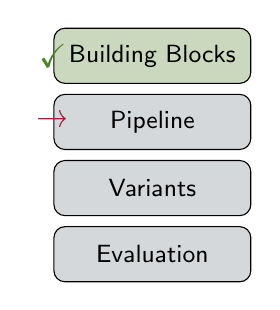
\begin{tikzpicture}[scale=0.7]
                % Progress indicator
                \foreach \i/\label/\col in {0/Building Blocks/TuebingenGreen, 1/Pipeline/TuebingenGray, 2/Variants/TuebingenGray, 3/Evaluation/TuebingenGray} {
                    \node[draw, fill=\col!30, rounded corners, minimum width=2.5cm, minimum height=0.7cm] at (0, -\i*1.2) {\small \label};
                }
                
                % Check mark on first
                \node[TuebingenGreen, font=\large] at (-1.8, 0) {\checkmark};
                
                % Arrow for current
                \node[TuebingenRot, font=\large] at (-1.8, -1.2) {→};
            \end{tikzpicture}
        \end{center}
    \end{columns}
\end{frame}

% ------------------------------------------------------------------------------
% II-D.1 Why RAG Exists
% ------------------------------------------------------------------------------

\begin{frame}{Why RAG Exists: The Parametric Memory Problem}
    \framesubtitle{Models are not databases}
    
    \vspace{0.2em}
    \begin{columns}[T]
        \column{0.48\textwidth}
        \textbf{The Problem with "Parametric Memory":}
        \begin{itemize}
            \setlength\itemsep{0.3em}
            \item LLMs store knowledge \textbf{in weights}
            \item Training data has a \textbf{cutoff date}
            \item Can't reliably recall \textbf{specific facts}
            \item No access to \textbf{your proprietary data}
            \item Can't cite \textbf{authoritative sources}
        \end{itemize}
        
        \vspace{0.3em}
        \textbf{What Happens Without RAG:}
        \begin{itemize}
            \setlength\itemsep{0.2em}
            \item "Who is our CFO?" → \textcolor{TuebingenRot}{Hallucination}
            \item "What's our refund policy?" → \textcolor{TuebingenRot}{Outdated info}
            \item "Show me Q3 numbers" → \textcolor{TuebingenRot}{Made up}
        \end{itemize}
        
        \column{0.48\textwidth}
        \textbf{RAG = Retrieval + Generation + Citations}
        
        \vspace{0.3em}
        \begin{center}
            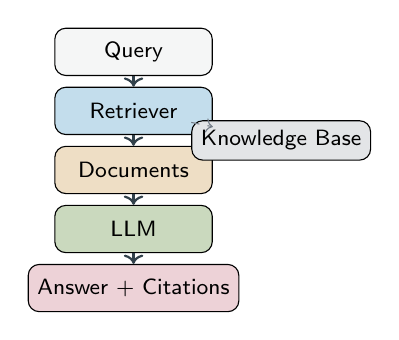
\begin{tikzpicture}[scale=0.75]
                % Query
                \node[draw, fill=TuebingenBeige, rounded corners, minimum width=2cm, minimum height=0.6cm] (query) at (0,3) {\footnotesize Query};
                
                % Retriever
                \node[draw, fill=TuebingenCyan!30, rounded corners, minimum width=2cm, minimum height=0.6cm] (retriever) at (0,2) {\footnotesize Retriever};
                
                % Documents
                \node[draw, fill=TuebingenGold!30, rounded corners, minimum width=2cm, minimum height=0.6cm] (docs) at (0,1) {\footnotesize Documents};
                
                % LLM
                \node[draw, fill=TuebingenGreen!30, rounded corners, minimum width=2cm, minimum height=0.6cm] (llm) at (0,0) {\footnotesize LLM};
                
                % Answer
                \node[draw, fill=TuebingenRot!20, rounded corners, minimum width=2cm, minimum height=0.6cm] (answer) at (0,-1) {\footnotesize Answer + Citations};
                
                % Arrows
                \draw[->, thick, TuebingenAnthrazit] (query) -- (retriever);
                \draw[->, thick, TuebingenAnthrazit] (retriever) -- (docs);
                \draw[->, thick, TuebingenAnthrazit] (docs) -- (llm);
                \draw[->, thick, TuebingenAnthrazit] (llm) -- (answer);
                
                % Knowledge base
                \node[draw, fill=TuebingenGray!20, rounded corners, minimum width=1.5cm, minimum height=0.5cm] (kb) at (2.5,1.5) {\footnotesize Knowledge Base};
                \draw[->, dashed, TuebingenGray] (kb) -- (retriever);
            \end{tikzpicture}
        \end{center}
        
        \vspace{0.3em}
        {\small\color{TuebingenGreen}\textbf{Key insight:} Retrieve relevant context at query time, don't rely on model's memory.}
    \end{columns}
\end{frame}

\begin{frame}{The Canonical RAG Pipeline: Overview}
    \framesubtitle{Nine stages from document to answer}

    \vspace{0.5em}
    \begin{center}
        \begin{tikzpicture}[scale=0.88, every node/.style={font=\footnotesize}]
            % Offline (Indexing) Block
            \node[draw, fill=TuebingenRot!20, rounded corners, minimum width=1.8cm, minimum height=0.8cm, align=center] (ingest) at (0,0) {1. Ingest};
            \node[draw, fill=TuebingenGold!20, rounded corners, minimum width=1.8cm, minimum height=0.8cm, align=center] (chunk) at (2.1,0) {2. Chunk};
            \node[draw, fill=TuebingenGreen!20, rounded corners, minimum width=1.8cm, minimum height=0.8cm, align=center] (embed) at (4.2,0) {3. Embed};

            \node[draw, very thick, fit=(ingest) (chunk) (embed), inner sep=0.4cm, label={[align=center, font=\scriptsize, yshift=1.05cm]above:\textbf{Offline} \\ (Indexing)}, color=TuebingenGray] (offlinebox) {};

            % Online (Query) Block
            \node[draw, fill=TuebingenCyan!20, rounded corners, minimum width=1.8cm, minimum height=0.8cm, align=center] (retrieve) at (6.7,0) {4. Retrieve};
            \node[draw, fill=TuebingenRot!30, rounded corners, minimum width=1.8cm, minimum height=0.8cm, align=center] (rerank) at (8.8,0) {5. Rerank};
            \node[draw, fill=TuebingenGold!30, rounded corners, minimum width=1.8cm, minimum height=0.8cm, align=center] (prompt) at (10.9,0) {6. Prompt};
            \node[draw, fill=TuebingenGreen!30, rounded corners, minimum width=1.8cm, minimum height=0.8cm, align=center] (generate) at (13,0) {7. Generate};
            \node[draw, fill=TuebingenCyan!30, rounded corners, minimum width=1.8cm, minimum height=0.8cm, align=center] (post) at (15.1,0) {8. Post-proc};
            \node[draw, fill=TuebingenAnthrazit!20, rounded corners, minimum width=1.8cm, minimum height=0.8cm, align=center] (feedback) at (17.2,0) {9. Feedback};

            \node[draw, very thick, fit=(retrieve) (rerank) (prompt) (generate) (post) (feedback), inner sep=0.45cm,
                  label={[align=center, font=\scriptsize, yshift=1.05cm]above:\textbf{Online} \\ (Query Time)}, color=TuebingenGray] (onlinebox) {};

            % Arrows
            \draw[->, thick] (ingest) -- (chunk);
            \draw[->, thick] (chunk) -- (embed);
            \draw[->, thick] (embed) -- (retrieve);
            \draw[->, thick] (retrieve) -- (rerank);
            \draw[->, thick] (rerank) -- (prompt);
            \draw[->, thick] (prompt) -- (generate);
            \draw[->, thick] (generate) -- (post);
            \draw[->, thick] (post) -- (feedback);

            % Feedback loop: from feedback to ingest
            \draw[->, dashed, TuebingenGray] (feedback.south) .. controls +(down:1.2cm) and +(down:1.2cm) .. (ingest.south);
        \end{tikzpicture}
    \end{center}

    \vspace{0.5em}
    \begin{columns}[T]
        \column{0.48\textwidth}
        \textbf{Offline (Indexing):}
        \begin{enumerate}
            \setlength\itemsep{0.2em}
            \item \textbf{Ingest:} Parse docs, extract metadata
            \item \textbf{Chunk:} Split into retrievable units
            \item \textbf{Embed:} Convert to vectors, index
        \end{enumerate}
        
        \column{0.48\textwidth}
        \textbf{Online (Query):}
        \begin{enumerate}
            \setlength\itemsep{0.2em}
            \setcounter{enumi}{3}
            \item \textbf{Retrieve:} Find similar chunks
            \item \textbf{Rerank:} Improve precision
            \item \textbf{Prompt:} Assemble context
            \item \textbf{Generate:} LLM produces answer
            \item \textbf{Post-process:} Validate, format
            \item \textbf{Feedback:} Log, evaluate, improve
        \end{enumerate}
    \end{columns}
\end{frame}

\begin{frame}{RAG Pipeline: Ingestion \& Chunking}
    \framesubtitle{The foundation that determines success or failure}
    
    \vspace{0.3em}
    \begin{columns}[T]
        \column{0.48\textwidth}
        \textbf{1. Ingestion — What to capture:}
        \begin{itemize}
            \setlength\itemsep{0.3em}
            \item \textbf{Content:} Text, tables, images
            \item \textbf{Metadata:} Owner, date, source, version
            \item \textbf{Permissions:} ACLs, classification level
            \item \textbf{Structure:} Headers, sections, hierarchy
        \end{itemize}
        
        \vspace{0.3em}
        {\color{TuebingenRot}\textbf{Common Failures:}}
        \begin{itemize}
            \setlength\itemsep{0.2em}
            \item Tables rendered as gibberish
            \item PDFs with OCR errors
            \item Missing permission metadata
            \item Stale documents not removed
        \end{itemize}
        
        \column{0.48\textwidth}
        \textbf{2. Chunking — Strategy matters:}
        
        \vspace{0.3em}
        \begin{tabular}{@{}ll@{}}
            \toprule
            \textbf{Strategy} & \textbf{Best For} \\
            \midrule
            Fixed-size & Simple, predictable \\
            Sentence-based & Natural boundaries \\
            Paragraph-based & Coherent units \\
            Section-based & Structured docs \\
            Semantic & Topic coherence \\
            Overlapping & Context preservation \\
            \bottomrule
        \end{tabular}
        
        \vspace{0.5em}
        {\small\color{TuebingenGray} \textbf{Rule of thumb:} Chunk size should match typical query scope. Too small → missing context. Too large → noise + cost.}
    \end{columns}
\end{frame}

\begin{frame}{RAG Pipeline: Embedding \& Indexing}
    \framesubtitle{Converting documents to searchable vectors}
    
    \vspace{0.3em}
    \begin{columns}[T]
        \column{0.48\textwidth}
        \textbf{3. Embedding:}
        \begin{itemize}
            \setlength\itemsep{0.4em}
            \item Convert each chunk to a dense vector
            \item Vector captures semantic meaning
            \item Similar content → similar vectors
            \item Typical dimensions: 384–1536
        \end{itemize}
        
        \vspace{0.3em}
        \textbf{Embedding Model Choice:}
        \begin{itemize}
            \setlength\itemsep{0.3em}
            \item General-purpose (OpenAI, Cohere)
            \item Domain-specific (legal, medical)
            \item Multilingual considerations
            \item Cost vs quality trade-off
        \end{itemize}
        
        \column{0.48\textwidth}
        \textbf{Indexing Options:}
        \begin{itemize}
            \setlength\itemsep{0.4em}
            \item \textbf{Dedicated vector DB:} Pinecone, Weaviate, Qdrant, Milvus
            \item \textbf{DB extension:} PostgreSQL + pgvector, Elasticsearch
            \item \textbf{In-memory:} FAISS for smaller datasets
        \end{itemize}
        
        \vspace{0.3em}
        \textbf{Key Decisions:}
        \begin{itemize}
            \setlength\itemsep{0.3em}
            \item Index type (HNSW, IVF, etc.)
            \item Metadata storage alongside vectors
            \item Refresh/update strategy
        \end{itemize}
    \end{columns}
    
    \vspace{0.5em}
    {\color{TuebingenGray}\textbf{Rule:} Store original text and metadata with vectors for traceability and filtering.}
\end{frame}

\begin{frame}{RAG Pipeline: Retrieval \& Reranking}
    \framesubtitle{Finding and prioritizing relevant content}
    
    \vspace{0.3em}
    \begin{columns}[T]
        \column{0.48\textwidth}
        \textbf{4. Retrieval:}
        \begin{itemize}
            \setlength\itemsep{0.4em}
            \item Query → embedding vector
            \item Find top-k similar chunks
            \item Apply filters (permissions, date, source)
        \end{itemize}
        
        \vspace{0.3em}
        {\color{TuebingenRot}\textbf{Recall vs Precision Trade-off:}}
        \begin{itemize}
            \setlength\itemsep{0.3em}
            \item High k → better recall, more noise
            \item Low k → might miss relevant info
            \item Solution: retrieve many, rerank to few
        \end{itemize}
        
        \column{0.48\textwidth}
        \textbf{5. Reranking:}
        \begin{itemize}
            \setlength\itemsep{0.4em}
            \item Take top-N candidates (e.g., 50)
            \item Score with cross-encoder model
            \item Return top-K highest (e.g., 5)
        \end{itemize}
        
        \vspace{0.3em}
        \textbf{Why Rerank?}
        \begin{itemize}
            \setlength\itemsep{0.3em}
            \item Embeddings = fast but approximate
            \item Cross-encoder = slower but precise
            \item Two-stage: speed + accuracy
        \end{itemize}
    \end{columns}
    
    \vspace{0.5em}
    \begin{theorembox}{Hybrid Retrieval}
        Combine \textbf{vector search} (semantic similarity) with \textbf{keyword search} (exact terms). \\
        Essential for: product IDs, legal terms, compliance language, proper nouns.
    \end{theorembox}
\end{frame}

\begin{frame}{RAG Pipeline: Prompt Assembly \& Generation}
    \framesubtitle{Combining context with the query}
    
    \vspace{0.3em}
    \begin{columns}[T]
        \column{0.48\textwidth}
        \textbf{6. Prompt Assembly:}
        
        \vspace{0.3em}
        Build the full prompt from components:
        \begin{itemize}
            \setlength\itemsep{0.4em}
            \item \textbf{System instructions:} Persona, constraints, tone
            \item \textbf{Retrieved context:} Chunks with source markers
            \item \textbf{User query:} The actual question
            \item \textbf{Output format:} JSON schema, structure requirements
        \end{itemize}
        
        \vspace{0.3em}
        {\small\color{TuebingenGray} Order matters: system → context → query → format}
        
        \column{0.48\textwidth}
        \textbf{7. Generation:}
        
        \vspace{0.3em}
        LLM produces the answer:
        \begin{itemize}
            \setlength\itemsep{0.4em}
            \item \textbf{Key instruction:} "Only use provided context"
            \item \textbf{Citation markers:} [Source 1], [Doc A]
            \item \textbf{Refusal behavior:} "I don't have information about..."
            \item \textbf{Confidence signals:} "Based on the policy..."
        \end{itemize}
        
        \vspace{0.3em}
        {\small\color{TuebingenGray} Good prompts prevent hallucination}
    \end{columns}
    
    \vspace{0.5em}
    \begin{center}
        \small\color{TuebingenRot} \textbf{Key insight:} The prompt template is a critical tuning lever. Iterate on it like code.
    \end{center}
\end{frame}

\begin{frame}{RAG Pipeline: Post-Processing \& Feedback}
    \framesubtitle{Validation and continuous improvement}
    
    \vspace{0.3em}
    \begin{columns}[T]
        \column{0.48\textwidth}
        \textbf{8. Post-Processing:}
        
        \vspace{0.3em}
        Validate and clean the output:
        \begin{itemize}
            \setlength\itemsep{0.4em}
            \item \textbf{Format validation:} JSON schema, required fields
            \item \textbf{Citation verification:} Do citations match sources?
            \item \textbf{PII scrubbing:} Remove leaked sensitive data
            \item \textbf{Safety checks:} Content policy compliance
            \item \textbf{Length/quality gates:} Reject poor responses
        \end{itemize}
        
        \column{0.48\textwidth}
        \textbf{9. Feedback Loop:}
        
        \vspace{0.3em}
        Enable continuous improvement:
        \begin{itemize}
            \setlength\itemsep{0.4em}
            \item \textbf{Logging:} Query, retrieval, response
            \item \textbf{User feedback:} Thumbs up/down, corrections
            \item \textbf{Evaluation dataset:} Build from real queries
            \item \textbf{Failure analysis:} Identify retrieval gaps
            \item \textbf{A/B testing:} Compare prompt variants
        \end{itemize}
    \end{columns}
    
    \vspace{0.5em}
    \begin{theorembox}{Executive Insight}
        The feedback loop is how RAG systems \textbf{improve over time}. \\
        Without it, you're flying blind—unable to know if quality is degrading.
    \end{theorembox}
\end{frame}

\begin{frame}{RAG Variant A: Naive RAG}
    \framesubtitle{Simple but limited}
    
    \vspace{0.3em}
    \begin{columns}[T]
        \column{0.55\textwidth}
        \textbf{How It Works:}
        \begin{enumerate}
            \setlength\itemsep{0.3em}
            \item Embed query
            \item Vector search → top-k chunks
            \item Stuff all chunks into prompt
            \item Generate answer
        \end{enumerate}
        
        \vspace{0.3em}
        \textbf{When It's Sufficient:}
        \begin{itemize}
            \setlength\itemsep{0.3em}
            \item Small, homogeneous document set
            \item Simple factual queries
            \item Low-stakes use cases
            \item Proof of concept / demos
        \end{itemize}
        
        \column{0.42\textwidth}
        {\color{TuebingenRot}\textbf{Failure Modes:}}
        \begin{itemize}
            \setlength\itemsep{0.3em}
            \item \textbf{Irrelevant retrieval:} Semantic similarity ≠ relevance
            \item \textbf{Hallucination despite context:} Model ignores or misinterprets
            \item \textbf{Poor chunking:} Context split across chunks
            \item \textbf{No ranking:} Garbage in first position
            \item \textbf{No permissions:} Returns unauthorized content
        \end{itemize}
    \end{columns}
    
    \vspace{0.3em}
    \begin{theorembox}{Executive Guidance}
        Naive RAG is a \textbf{starting point}, not a production architecture. \\
        Fine for demos, but enterprise deployment requires the variants that follow.
    \end{theorembox}
\end{frame}

\begin{frame}{RAG Variant B: Hybrid Retrieval}
    \framesubtitle{Keyword + Vector = Best of both}
    
    \vspace{0.3em}
    \begin{columns}[T]
        \column{0.48\textwidth}
        \textbf{The Problem:}
        \begin{itemize}
            \setlength\itemsep{0.3em}
            \item Vector search: great for \textbf{semantic} similarity
            \item But fails on: \textbf{exact terms}, IDs, codes, names
            \item "Find policy ABC-123" → vector search returns wrong policy
        \end{itemize}
        
        \vspace{0.3em}
        \textbf{The Solution:}
        \begin{itemize}
            \setlength\itemsep{0.3em}
            \item Run \textbf{both} keyword (BM25) and vector search
            \item Combine results with reciprocal rank fusion
            \item Rerank the combined set
        \end{itemize}
        
        \column{0.48\textwidth}
        \textbf{When to Use Hybrid:}
        \begin{itemize}
            \setlength\itemsep{0.3em}
            \item \textbf{Legal/compliance:} Exact clause references
            \item \textbf{Technical docs:} Error codes, product IDs
            \item \textbf{Financial:} Account numbers, ticker symbols
            \item \textbf{HR:} Policy numbers, form names
        \end{itemize}
        
        \vspace{0.3em}
        \textbf{Implementation:}
        \begin{itemize}
            \setlength\itemsep{0.2em}
            \item Elasticsearch + vector plugin
            \item PostgreSQL + pgvector + FTS
            \item Dedicated hybrid search services
        \end{itemize}
    \end{columns}
    
    \vspace{0.5em}
    {\color{TuebingenGray}\textbf{Rule of thumb:} If your corpus has important exact-match terms, hybrid is not optional.}
\end{frame}

\begin{frame}{RAG Variant C: Hierarchical RAG}
    \framesubtitle{Coarse-to-fine retrieval}
    
    \vspace{0.3em}
    \begin{columns}[T]
        \column{0.48\textwidth}
        \textbf{The Problem:}
        \begin{itemize}
            \setlength\itemsep{0.3em}
            \item Flat retrieval loses document structure
            \item Similar passages from different docs get mixed
            \item Hard to trace "which document said this"
        \end{itemize}
        
        \vspace{0.3em}
        \textbf{Hierarchical Approach:}
        \begin{enumerate}
            \setlength\itemsep{0.3em}
            \item \textbf{Level 1:} Retrieve relevant \textbf{documents}
            \item \textbf{Level 2:} Within docs, retrieve \textbf{sections}
            \item \textbf{Level 3:} Within sections, retrieve \textbf{passages}
        \end{enumerate}
        
        \column{0.48\textwidth}
        \begin{center}
            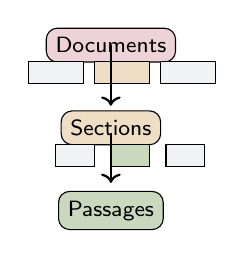
\begin{tikzpicture}[scale=0.7]
                % Documents level
                \node[draw, fill=TuebingenRot!20, rounded corners] (docs) at (0,2.5) {\footnotesize Documents};
                \draw[fill=TuebingenGray!10] (-1.5,1.8) rectangle (-0.5,2.2);
                \draw[fill=TuebingenGold!30] (-0.3,1.8) rectangle (0.7,2.2);
                \draw[fill=TuebingenGray!10] (0.9,1.8) rectangle (1.9,2.2);
                
                % Sections level
                \node[draw, fill=TuebingenGold!30, rounded corners] (secs) at (0,1) {\footnotesize Sections};
                \draw[fill=TuebingenGray!10] (-1,0.3) rectangle (-0.3,0.7);
                \draw[fill=TuebingenGreen!30] (0,0.3) rectangle (0.7,0.7);
                \draw[fill=TuebingenGray!10] (1,0.3) rectangle (1.7,0.7);
                
                % Passages level
                \node[draw, fill=TuebingenGreen!30, rounded corners] (pass) at (0,-0.5) {\footnotesize Passages};
                
                % Arrows
                \draw[->, thick] (0,2.5) -- (0,1.4);
                \draw[->, thick] (0,0.9) -- (0,0);
            \end{tikzpicture}
        \end{center}
        
        \vspace{0.3em}
        \textbf{Benefits:}
        \begin{itemize}
            \setlength\itemsep{0.2em}
            \item Better traceability
            \item Reduces context noise
            \item Respects document boundaries
        \end{itemize}
    \end{columns}
    
    \vspace{0.3em}
    {\color{TuebingenGray}\textbf{Best for:} Large document collections with clear structure (manuals, policies, legal).}
\end{frame}

\begin{frame}{RAG Variant D: Multi-Query RAG}
    \framesubtitle{Multiple perspectives, better recall}
    
    \vspace{0.3em}
    \begin{columns}[T]
        \column{0.48\textwidth}
        \textbf{The Problem:}
        \begin{itemize}
            \setlength\itemsep{0.3em}
            \item User query may be ambiguous
            \item Single embedding may miss relevant docs
            \item Different phrasings match different content
        \end{itemize}
        
        \vspace{0.3em}
        \textbf{Multi-Query Approach:}
        \begin{enumerate}
            \setlength\itemsep{0.3em}
            \item LLM generates 3-5 query variations
            \item Run retrieval for each variation
            \item Merge and deduplicate results
            \item Rerank combined set
        \end{enumerate}
        
        \column{0.48\textwidth}
        \textbf{Example:}
        
        \vspace{0.3em}
        \textbf{Original:} "How do I get reimbursed?"
        
        \vspace{0.2em}
        \textbf{Generated variations:}
        \begin{itemize}
            \setlength\itemsep{0.2em}
            \item "expense reimbursement process"
            \item "submit expenses for payment"
            \item "travel expense policy"
            \item "reimbursement form submission"
        \end{itemize}
        
        \vspace{0.3em}
        {\color{TuebingenRot}\textbf{Trade-offs:}}
        \begin{itemize}
            \setlength\itemsep{0.2em}
            \item Higher latency (multiple retrievals)
            \item Higher cost (LLM for query gen)
            \item Risk of query drift
        \end{itemize}
    \end{columns}
    
    \vspace{0.3em}
    {\color{TuebingenGray}\textbf{Best for:} Ambiguous queries, diverse document language, high-stakes answers where recall matters.}
\end{frame}

\begin{frame}{RAG Variant E: GraphRAG / Knowledge Graph}
    \framesubtitle{Beyond embedding similarity}
    
    \vspace{0.3em}
    \begin{columns}[T]
        \column{0.48\textwidth}
        \textbf{The Problem:}
        \begin{itemize}
            \setlength\itemsep{0.3em}
            \item Embeddings capture similarity, not relationships
            \item "Who reports to whom?" needs structure
            \item Multi-hop reasoning across entities
        \end{itemize}
        
        \vspace{0.3em}
        \textbf{GraphRAG Approach:}
        \begin{enumerate}
            \setlength\itemsep{0.3em}
            \item Extract \textbf{entities} from documents
            \item Build \textbf{relationships} (owns, reports-to, depends-on)
            \item Query combines graph traversal + vector search
            \item Context includes entity relationships
        \end{enumerate}
        
        \column{0.48\textwidth}
        \begin{center}
            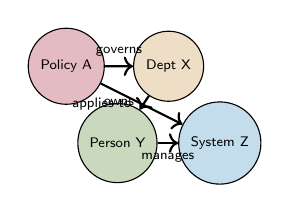
\begin{tikzpicture}[scale=0.65]
                % Nodes
                \node[draw, circle, fill=TuebingenRot!30, minimum size=0.8cm, font=\tiny] (a) at (0,2) {Policy A};
                \node[draw, circle, fill=TuebingenGold!30, minimum size=0.8cm, font=\tiny] (b) at (2,2) {Dept X};
                \node[draw, circle, fill=TuebingenGreen!30, minimum size=0.8cm, font=\tiny] (c) at (1,0.5) {Person Y};
                \node[draw, circle, fill=TuebingenCyan!30, minimum size=0.8cm, font=\tiny] (d) at (3,0.5) {System Z};
                
                % Edges
                \draw[->, thick] (a) -- node[above, font=\tiny] {governs} (b);
                \draw[->, thick] (b) -- node[left, font=\tiny] {owns} (c);
                \draw[->, thick] (c) -- node[below, font=\tiny] {manages} (d);
                \draw[->, thick] (a) -- node[left, font=\tiny] {applies-to} (d);
            \end{tikzpicture}
        \end{center}
        
        \vspace{0.3em}
        \textbf{Strong For:}
        \begin{itemize}
            \setlength\itemsep{0.2em}
            \item Organizational knowledge
            \item Ownership and accountability
            \item Dependency tracking
            \item Compliance traceability
        \end{itemize}
    \end{columns}
    
    \vspace{0.3em}
    {\color{TuebingenRot}\textbf{Investment required:} Entity extraction, schema design, ongoing maintenance. High value but high cost.}
\end{frame}

\begin{frame}{RAG Variant F: Text-to-SQL / Structured RAG}
    \framesubtitle{When the answer lives in a database}
    
    \vspace{0.3em}
    \begin{columns}[T]
        \column{0.48\textwidth}
        \textbf{The Problem:}
        \begin{itemize}
            \setlength\itemsep{0.3em}
            \item Many enterprise answers are in \textbf{databases}
            \item "What was Q3 revenue?" needs SQL, not document retrieval
            \item RAG over documents can't give precise KPIs
        \end{itemize}
        
        \vspace{0.3em}
        \textbf{Text-to-SQL Approach:}
        \begin{enumerate}
            \setlength\itemsep{0.3em}
            \item Natural language query
            \item LLM generates SQL (with schema context)
            \item Execute SQL against database
            \item LLM explains results
        \end{enumerate}
        
        \column{0.48\textwidth}
        \textbf{Example Flow:}
        
        \vspace{0.3em}
        \textbf{User:} "Top 5 customers by revenue this quarter"
        
        \vspace{0.2em}
        \textbf{Generated SQL:}
        \begin{codebox}
            SELECT customer, SUM(revenue)\\
            FROM orders\\
            WHERE quarter = 'Q3'\\
            GROUP BY customer\\
            ORDER BY 2 DESC LIMIT 5;
        \end{codebox}
        
        \vspace{0.2em}
        {\color{TuebingenRot}\textbf{Critical:}}
        \begin{itemize}
            \setlength\itemsep{0.2em}
            \item SQL validation before execution
            \item Permission checks
            \item Query cost/timeout limits
        \end{itemize}
    \end{columns}
    
    \vspace{0.3em}
    {\color{TuebingenGray}\textbf{Best for:} Analytics, KPIs, operational metrics where \textbf{correctness} matters and data is structured.}
\end{frame}

\begin{frame}{RAG Variant G: Code/Repository RAG}
    \framesubtitle{Specialized retrieval for software artifacts}
    
    \vspace{0.3em}
    \begin{columns}[T]
        \column{0.48\textwidth}
        \textbf{The Challenge:}
        \begin{itemize}
            \setlength\itemsep{0.3em}
            \item Code has different structure than prose
            \item Functions, classes, imports, call graphs
            \item Need to retrieve \textbf{relevant code context}
        \end{itemize}
        
        \vspace{0.3em}
        \textbf{What to Index:}
        \begin{itemize}
            \setlength\itemsep{0.3em}
            \item Source code (functions, classes)
            \item Documentation (docstrings, README)
            \item Architecture Decision Records (ADRs)
            \item Issue tickets and PRs
            \item API specifications
        \end{itemize}
        
        \column{0.48\textwidth}
        \textbf{Chunking Strategies for Code:}
        \begin{itemize}
            \setlength\itemsep{0.4em}
            \item \textbf{Function-level:} Natural code units
            \item \textbf{Class-level:} Object context
            \item \textbf{File-level:} Module context
            \item \textbf{Dependency-aware:} Include imports
            \item \textbf{Call-graph aware:} Related functions
        \end{itemize}
        
        \vspace{0.3em}
        \textbf{Use Cases:}
        \begin{itemize}
            \setlength\itemsep{0.2em}
            \item "How does authentication work?"
            \item "Find usages of deprecated API"
            \item "What does this error mean?"
        \end{itemize}
    \end{columns}
    
    \vspace{0.3em}
    {\color{TuebingenGray}\textbf{Key insight:} Code assistants are RAG systems with specialized indexing and retrieval for software.}
\end{frame}

\begin{frame}{Enterprise RAG: Permission Enforcement}
    \framesubtitle{Preventing unauthorized data exposure}
    
    \vspace{0.3em}
    \begin{columns}[T]
        \column{0.48\textwidth}
        {\color{TuebingenRot}\textbf{The Risk:}}
        
        \vspace{0.3em}
        RAG can expose unauthorized data:
        \begin{itemize}
            \setlength\itemsep{0.4em}
            \item "Summarize all HR docs" → returns confidential salary info
            \item "What's in the board minutes?" → leaks M\&A plans
            \item UI-level permissions are \textbf{not enough}
        \end{itemize}
        
        \column{0.48\textwidth}
        \textbf{Permission Enforcement Points:}
        
        \vspace{0.3em}
        \begin{itemize}
            \setlength\itemsep{0.5em}
            \item \textbf{At indexing:} Store ACLs with every chunk
            \item \textbf{At retrieval:} Filter by user's permissions
            \item \textbf{At generation:} Don't mix authorization levels
            \item \textbf{At output:} Verify no permission escalation
        \end{itemize}
    \end{columns}
    
    \vspace{0.5em}
    \begin{theorembox}{Implementation Principle}
        Permissions must be enforced at the \textbf{retrieval layer}, not just the UI. \\
        The RAG system inherits the document's access controls.
    \end{theorembox}
\end{frame}

\begin{frame}{Enterprise RAG: Audit Requirements}
    \framesubtitle{What to log for every query}
    
    \vspace{0.5em}
    \textbf{Every Query Must Log:}
    
    \vspace{0.3em}
    \begin{columns}[T]
        \column{0.48\textwidth}
        \begin{itemize}
            \setlength\itemsep{0.6em}
            \item \textbf{Who asked?} User identity, role
            \item \textbf{What was retrieved?} Source IDs, chunk text
            \item \textbf{Why these sources?} Relevance scores
        \end{itemize}
        
        \column{0.48\textwidth}
        \begin{itemize}
            \setlength\itemsep{0.6em}
            \item \textbf{What was generated?} Full response
            \item \textbf{When?} Timestamp, latency
            \item \textbf{Token usage?} Cost tracking
        \end{itemize}
    \end{columns}
    
    \vspace{0.5em}
    \begin{theorembox}{Executive Mandate}
        Every RAG deployment must answer: \textbf{"What sources influenced this answer?"} \\
        If you can't answer that, you're not ready for production.
    \end{theorembox}
\end{frame}

\begin{frame}{Enterprise RAG: Why Audit?}
    \framesubtitle{Audit is non-negotiable in production}
    \vspace{0.5em}
    \begin{itemize}
        \item \textbf{Traceability:} Know exactly which sources were used for every answer.
        \item \textbf{Compliance:} Prove data handling meets legal and policy requirements.
        \item \textbf{Debugging:} Quickly identify and fix root causes of errors.
    \end{itemize}
    \vspace{0.5em}
    {\color{TuebingenGray}\textbf{Implementation:} Log every query, answer, and source with a unique query ID.}
\end{frame}

\begin{frame}{RAG: Precise Evaluation Metrics}
    \framesubtitle{Objectively assess retrieval and generation}
    \vspace{0.5em}
    \textbf{Retrieval:}
    \begin{itemize}
        \item \textbf{Recall@k:} Are the right docs included in top results?
        \item \textbf{Precision@k:} How much noise is present?
    \end{itemize}
    \textbf{Generation:}
    \begin{itemize}
        \item \textbf{Groundedness:} Only claims supported by retrieved docs.
        \item \textbf{Citation Accuracy:} Every citation matches its claim.
        \item \textbf{Factuality \& Completeness:} All info is correct and fully answers the question.
    \end{itemize}
    \vspace{0.5em}
    {\color{TuebingenGray}Evaluate retrieval and generation independently.}
\end{frame}

\begin{frame}{RAG: Example Query Trace}
    \framesubtitle{Every answer must be auditable}
    \vspace{0.3em}
    \textbf{Example:}
    \begin{itemize}
        \item \textbf{User query:} "What is our remote work policy?"
        \item \textbf{Retrieved docs:} HR-Policy.pdf, Exception-Approval.docx (scored for relevance)
        \item \textbf{Generated answer:} Policy summary and approval process with document citations
        \item \textbf{Log:} Query ID, user, timestamp, sources, confidence, final answer
    \end{itemize}
    \vspace{0.5em}
    {\color{TuebingenGreen}\textbf{Key:} Every answer should be fully traceable to sources via logs.}
\end{frame}

\begin{frame}{RAG: Production-Ready Checklist}
    \framesubtitle{Essentials for enterprise deployment}
    \vspace{0.5em}
    \begin{itemize}
        \item \textbf{Permissions:} Enforced at retrieval, not just UI.
        \item \textbf{Audit:} Source-to-answer logging for every query.
        \item \textbf{Evaluation:} Objective metrics and monitoring in place.
        \item \textbf{Feedback:} Users can rate answers and see improvements.
    \end{itemize}
    \vspace{0.5em}
    \begin{theorembox}{If any box is missing, it's not enterprise RAG.}
    \end{theorembox}

\end{frame}

% ==============================================================================
% PART II-E: BENCHMARKING, TESTING, MONITORING (10 minutes)
% ==============================================================================

\begin{frame}{Part II-E: Benchmarking, Testing \& Monitoring}
    \framesubtitle{10 minutes — The discipline that separates production from prototype}
    
    \vspace{0.5em}
    \begin{center}
        {\Large\color{TuebingenRot} Evaluation Discipline}
        
        \vspace{0.3em}
        {\color{TuebingenGray} How to know if your AI system actually works}
    \end{center}
    
    \vspace{0.5em}
    \textbf{What We'll Cover:}
    \begin{enumerate}
        \setlength\itemsep{0.3em}
        \item Why benchmarks matter — and their limits
        \item Train/validation/test splits — the foundation of trust
        \item Production monitoring — because deployment is just the beginning
    \end{enumerate}
    
    \vspace{0.3em}
    \begin{theorembox}{Why This Matters}
        Without rigorous evaluation, you can't distinguish a \textbf{working system} from a \textbf{lucky demo}. \\
        Evaluation governance is as important as model selection.
    \end{theorembox}
\end{frame}

\begin{frame}{Why Benchmarks Matter}
    \framesubtitle{The common language of AI capabilities}
    
    \vspace{0.5em}
    \textbf{Benchmarks Drive Decisions:}
    \begin{itemize}
        \setlength\itemsep{0.5em}
        \item \textbf{Vendor selection:} "Model X scores 90\% on MMLU"
        \item \textbf{Progress tracking:} "We improved 5\% on our task"
        \item \textbf{Research direction:} Community focuses on benchmark gaps
        \item \textbf{Investment:} Benchmark gains attract funding
    \end{itemize}
    
    \vspace{0.5em}
    \textbf{Common Benchmarks:}
    \begin{itemize}
        \setlength\itemsep{0.4em}
        \item \textbf{MMLU:} Multi-task language understanding
        \item \textbf{HumanEval:} Code generation accuracy
        \item \textbf{MATH:} Mathematical reasoning
        \item \textbf{TruthfulQA:} Factual accuracy
    \end{itemize}
\end{frame}

\begin{frame}{Benchmarks: The Critical Caveat}
    \framesubtitle{Why benchmark scores don't tell the whole story}
    
    \vspace{0.5em}
    \begin{center}
        {\Large\color{TuebingenRot} Benchmark performance $\neq$ Your business task performance}
    \end{center}
    
    \vspace{0.5em}
    \textbf{Why The Gap Exists:}
    \begin{itemize}
        \setlength\itemsep{0.5em}
        \item Your data distribution differs from benchmark data
        \item Your success criteria differ from benchmark metrics
        \item Your failure costs differ from benchmark assumptions
        \item Benchmark contamination in model training
    \end{itemize}
    
    \vspace{0.5em}
    \begin{theorembox}{Executive Implication}
        Use benchmarks for \textbf{initial screening}, but \textbf{build your own evaluation set} for deployment decisions. \\
        A model that excels on benchmarks may fail on your specific use case.
    \end{theorembox}
\end{frame}

\begin{frame}{Train / Validation / Test Splits}
    \framesubtitle{The foundation of trustworthy evaluation}
    
    \vspace{0.3em}
    \begin{columns}[T]
        \column{0.55\textwidth}
        \textbf{The Three-Way Split:}
        
        \vspace{0.3em}
        \begin{center}
            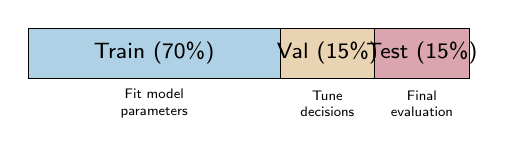
\begin{tikzpicture}[scale=0.8]
                % Data bar
                \draw[fill=TuebingenCyan!40] (0,0) rectangle (4,0.8);
                \draw[fill=TuebingenGold!40] (4,0) rectangle (5.5,0.8);
                \draw[fill=TuebingenRot!40] (5.5,0) rectangle (7,0.8);
                
                % Labels
                \node[font=\footnotesize] at (2, 0.4) {Train (70\%)};
                \node[font=\footnotesize] at (4.75, 0.4) {Val (15\%)};
                \node[font=\footnotesize] at (6.25, 0.4) {Test (15\%)};
                
                % Purposes
                \node[font=\tiny, align=center] at (2, -0.4) {Fit model\\parameters};
                \node[font=\tiny, align=center] at (4.75, -0.4) {Tune\\decisions};
                \node[font=\tiny, align=center] at (6.25, -0.4) {Final\\evaluation};
            \end{tikzpicture}
        \end{center}
        
        \vspace{0.5em}
        \textbf{Purpose of Each:}
        \begin{itemize}
            \setlength\itemsep{0.3em}
            \item \textbf{Training:} Model learns from this data
            \item \textbf{Validation:} Guide hyperparameter choices, early stopping
            \item \textbf{Test:} Final, unbiased performance estimate
        \end{itemize}
        
        \column{0.42\textwidth}
        {\color{TuebingenRot}\textbf{Leakage — The Silent Killer:}}
        \begin{itemize}
            \setlength\itemsep{0.4em}
            \item \textbf{Temporal:} Future data in training
            \item \textbf{Identity:} Same customer in train/test
            \item \textbf{Duplicate:} Same example appears twice
            \item \textbf{Feature:} Target encoded in features
        \end{itemize}
        
        \vspace{0.3em}
        \textbf{Symptoms of Leakage:}
        \begin{itemize}
            \setlength\itemsep{0.2em}
            \item "Too good to be true" test scores
            \item Model fails in production
            \item Performance degrades over time
        \end{itemize}
    \end{columns}
    
    \vspace{0.3em}
    {\color{TuebingenGray}\textbf{Rule:} Test set should \textbf{never} influence any decision during development. Touch it once, at the end.}
\end{frame}

\begin{frame}{Evaluation Governance: Access Control}
    \framesubtitle{Who can see what, when}
    
    \vspace{0.5em}
    \textbf{Data Access Policy:}
    \begin{itemize}
        \setlength\itemsep{0.6em}
        \item \textbf{Training data:} Available to developers
        \item \textbf{Validation data:} Available during development
        \item \textbf{Test data:} \textcolor{TuebingenRot}{Restricted access only}
        \item \textbf{Test results:} Run by independent party
    \end{itemize}
    
    \vspace{0.5em}
    \textbf{Why Governance Matters:}
    \begin{itemize}
        \setlength\itemsep{0.5em}
        \item Repeated test usage → overfitting to test set
        \item Public leaderboards incentivize gaming
        \item Business decisions need unbiased performance estimates
    \end{itemize}
\end{frame}

\begin{frame}{Evaluation Governance: Process}
    \framesubtitle{Practical implementation steps}
    
    \vspace{0.5em}
    \textbf{Practical Process:}
    \begin{enumerate}
        \setlength\itemsep{0.5em}
        \item Create test set at project start
        \item Lock it away (separate repo/access controls)
        \item Develop using train + validation only
        \item Run test evaluation \textbf{once} for final go/no-go decision
        \item Document results, don't iterate on test performance
    \end{enumerate}
    
    \vspace{0.5em}
    \textbf{For LLMs/RAG Systems:}
    \begin{itemize}
        \setlength\itemsep{0.4em}
        \item Create "golden set" of Q/A pairs
        \item Expert-validated reference answers
        \item Versioned and maintained over time
    \end{itemize}
\end{frame}

\begin{frame}{Production Monitoring: Alerts \& Pipeline}
    \framesubtitle{When to act and how data flows}
    
    \vspace{0.5em}
    \textbf{Alert Thresholds:}
    \begin{itemize}
        \setlength\itemsep{0.5em}
        \item \textcolor{TuebingenGold}{Warning:} 10\% drop in user satisfaction
        \item \textcolor{TuebingenRot}{Critical:} Retrieval failure rate > 5\%
        \item \textcolor{TuebingenRot}{Critical:} PII detected in outputs
        \item \textcolor{TuebingenGold}{Warning:} Latency p95 > 5 seconds
    \end{itemize}
    
    \vspace{0.5em}
    \textbf{The Monitoring Stack:}
    \begin{center}
        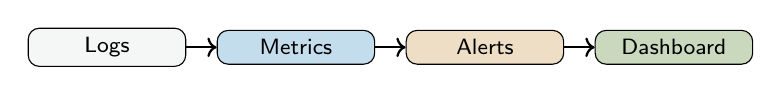
\begin{tikzpicture}[scale=0.8, font=\footnotesize]
            \node[draw, fill=TuebingenBeige, rounded corners, minimum width=2cm] (logs) at (0,0) {Logs};
            \node[draw, fill=TuebingenCyan!30, rounded corners, minimum width=2cm] (metrics) at (3,0) {Metrics};
            \node[draw, fill=TuebingenGold!30, rounded corners, minimum width=2cm] (alerts) at (6,0) {Alerts};
            \node[draw, fill=TuebingenGreen!30, rounded corners, minimum width=2cm] (dashboard) at (9,0) {Dashboard};
            
            \draw[->, thick] (logs) -- (metrics);
            \draw[->, thick] (metrics) -- (alerts);
            \draw[->, thick] (alerts) -- (dashboard);
        \end{tikzpicture}
    \end{center}
\end{frame}

\begin{frame}{Act II Summary: Technical Foundations}
    \framesubtitle{What executives now understand about how AI works}
    
    \vspace{0.5em}
    \textbf{Part A — ML Foundations:}
    \begin{itemize}
        \setlength\itemsep{0.4em}
        \item Supervised/unsupervised/RL taxonomy
        \item Classical methods still valuable
        \item Right tool for right problem
    \end{itemize}
    
    \vspace{0.3em}
    \textbf{Part B — Deep Learning:}
    \begin{itemize}
        \setlength\itemsep{0.4em}
        \item Learned representations are key
        \item Optimization is about generalization
        \item Failure modes are predictable
    \end{itemize}
    
    \vspace{0.3em}
    \textbf{Part C — Transformers:}
    \begin{itemize}
        \setlength\itemsep{0.4em}
        \item Embeddings enable semantic search
        \item Attention enables context understanding
        \item Context windows have trade-offs
    \end{itemize}
\end{frame}

\begin{frame}{Act II Summary: Enterprise Systems}
    \framesubtitle{RAG, evaluation, and production readiness}
    
    \vspace{0.5em}
    \textbf{Part D — RAG Systems:}
    \begin{itemize}
        \setlength\itemsep{0.5em}
        \item RAG grounds LLMs in your data
        \item Multiple variants for different needs
        \item Permissions and audit are mandatory
    \end{itemize}
    
    \vspace{0.5em}
    \textbf{Part E — Evaluation:}
    \begin{itemize}
        \setlength\itemsep{0.5em}
        \item Benchmarks ≠ your task performance
        \item Test set governance prevents self-deception
        \item Production monitoring is continuous
    \end{itemize}
    
    \vspace{0.5em}
    \begin{theorembox}{The Meta-Lesson}
        Modern AI is \textbf{systems engineering}: model + retrieval + evaluation + monitoring. \\
        Success requires \textbf{all} components, not just a good model.
    \end{theorembox}
    
    \vspace{0.3em}
    {\color{TuebingenGray}\textbf{Next:} Act III — How to apply these systems to create business value.}
\end{frame}
% Act III — Business Application Patterns and Value (70 minutes)
% ==============================================================================
\section{Business Application Patterns}

% ==============================================================================
% SECTION 3.1: PATTERN CATALOG
% ==============================================================================

\begin{frame}{Act III: Business Application Patterns}
    \framesubtitle{70 minutes — From technical understanding to business value}
    
    \vspace{0.5em}
    \begin{center}
        {\Large\color{TuebingenRot} Converting AI Capabilities into Business Outcomes}
        
        \vspace{0.3em}
        {\color{TuebingenGray} Six proven patterns for enterprise AI deployment}
    \end{center}
    
    \vspace{0.5em}
    \textbf{What We'll Cover:}
    \begin{enumerate}
        \setlength\itemsep{0.4em}
        \item Pattern catalog overview
        \item Pattern 1: Enterprise knowledge assistant (RAG)
        \item Pattern 2: Customer support augmentation
        \item Pattern 3: Document \& workflow automation
        \item Pattern 4: Software engineering acceleration
        \item Pattern 5: Decision intelligence
        \item Pattern 6: Operations and quality
        \item Why pilots fail and what success looks like
    \end{enumerate}
    
    \vspace{0.3em}
    \begin{theorembox}{Purpose of This Act}
        Apply Act II's technical foundation to templates executives can \textbf{fund}, \textbf{govern}, and \textbf{scale}.
    \end{theorembox}
\end{frame}

\begin{frame}{The Six Enterprise AI Patterns}
    \framesubtitle{A taxonomy of proven applications}
    
    \vspace{0.3em}
    \begin{center}
        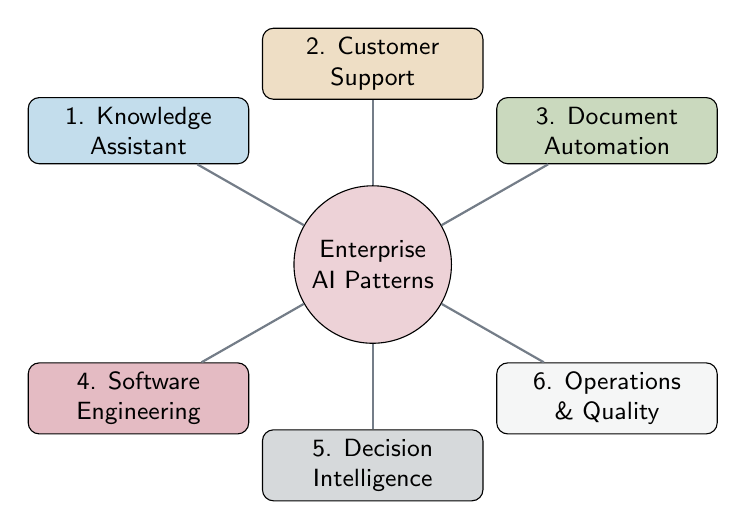
\begin{tikzpicture}[scale=0.85, every node/.style={font=\small}]
            % Center node
            \node[draw, circle, fill=TuebingenRot!20, minimum size=2cm, align=center] (center) at (0,0) {Enterprise\\AI Patterns};
            
            % Surrounding nodes
            \node[draw, rounded corners, fill=TuebingenCyan!30, minimum width=2.8cm, minimum height=0.8cm, align=center] (p1) at (-3.5, 2) {1. Knowledge\\Assistant};
            \node[draw, rounded corners, fill=TuebingenGold!30, minimum width=2.8cm, minimum height=0.8cm, align=center] (p2) at (0, 3) {2. Customer\\Support};
            \node[draw, rounded corners, fill=TuebingenGreen!30, minimum width=2.8cm, minimum height=0.8cm, align=center] (p3) at (3.5, 2) {3. Document\\Automation};
            \node[draw, rounded corners, fill=TuebingenRot!30, minimum width=2.8cm, minimum height=0.8cm, align=center] (p4) at (-3.5, -2) {4. Software\\Engineering};
            \node[draw, rounded corners, fill=TuebingenAnthrazit!20, minimum width=2.8cm, minimum height=0.8cm, align=center] (p5) at (0, -3) {5. Decision\\Intelligence};
            \node[draw, rounded corners, fill=TuebingenBeige, minimum width=2.8cm, minimum height=0.8cm, align=center] (p6) at (3.5, -2) {6. Operations\\\& Quality};
            
            % Lines
            \draw[thick, TuebingenGray] (center) -- (p1);
            \draw[thick, TuebingenGray] (center) -- (p2);
            \draw[thick, TuebingenGray] (center) -- (p3);
            \draw[thick, TuebingenGray] (center) -- (p4);
            \draw[thick, TuebingenGray] (center) -- (p5);
            \draw[thick, TuebingenGray] (center) -- (p6);
        \end{tikzpicture}
    \end{center}
    
    \vspace{0.3em}
    {\color{TuebingenGray}\textbf{Key insight:} Each pattern has distinct architecture, ROI levers, risks, and governance needs. One size does not fit all.}
\end{frame}

% ==============================================================================
% SECTION 3.2: PATTERN 1 — ENTERPRISE KNOWLEDGE ASSISTANT
% ==============================================================================

\begin{frame}{Pattern 1: Enterprise Knowledge Assistant}
    \framesubtitle{RAG-powered internal knowledge access}
    
    \vspace{0.3em}
    \begin{columns}[T]
        \column{0.48\textwidth}
        \textbf{What It Is:}
        \begin{itemize}
            \setlength\itemsep{0.3em}
            \item Natural language Q\&A over internal knowledge
            \item RAG architecture with citations
            \item Self-service for employees
        \end{itemize}
        
        \vspace{0.3em}
        \textbf{Use Cases:}
        \begin{itemize}
            \setlength\itemsep{0.3em}
            \item \textbf{HR:} Policies, benefits, procedures
            \item \textbf{IT:} Troubleshooting, how-to guides
            \item \textbf{Legal:} Compliance, contract terms
            \item \textbf{Product:} Specs, documentation
            \item \textbf{Sales:} Competitive intel, pricing
        \end{itemize}
        
        \column{0.48\textwidth}
        \textbf{Architecture:}
        \begin{center}
            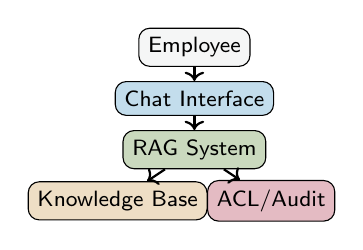
\begin{tikzpicture}[scale=0.65, font=\footnotesize]
                \node[draw, fill=TuebingenBeige, rounded corners] (user) at (0,2.5) {Employee};
                \node[draw, fill=TuebingenCyan!30, rounded corners] (chat) at (0,1.5) {Chat Interface};
                \node[draw, fill=TuebingenGreen!30, rounded corners] (rag) at (0,0.5) {RAG System};
                \node[draw, fill=TuebingenGold!30, rounded corners] (kb) at (-1.5,-0.5) {Knowledge Base};
                \node[draw, fill=TuebingenRot!30, rounded corners] (acl) at (1.5,-0.5) {ACL/Audit};
                
                \draw[->, thick] (user) -- (chat);
                \draw[->, thick] (chat) -- (rag);
                \draw[->, thick] (rag) -- (kb);
                \draw[->, thick] (rag) -- (acl);
            \end{tikzpicture}
        \end{center}
        
        \vspace{0.3em}
        \textbf{Key Components:}
        \begin{itemize}
            \setlength\itemsep{0.2em}
            \item Document ingestion pipeline
            \item Vector + keyword search
            \item Permission-aware retrieval
            \item Citation generation
        \end{itemize}
    \end{columns}
\end{frame}

\begin{frame}{Knowledge Assistant: ROI Levers}
    \framesubtitle{Where the value comes from}
    
    \vspace{0.3em}
    \begin{columns}[T]
        \column{0.48\textwidth}
        \textbf{Time Savings:}
        \begin{itemize}
            \setlength\itemsep{0.4em}
            \item \textbf{Time-to-answer:} Minutes → seconds
            \item \textbf{Search efficiency:} Find vs hunt
            \item \textbf{Onboarding:} Self-service learning
            \item \textbf{Expert availability:} Reduce interruptions
        \end{itemize}
        
        \vspace{0.3em}
        \textbf{Typical Metrics:}
        \begin{itemize}
            \setlength\itemsep{0.3em}
            \item Avg query resolution time
            \item Ticket deflection rate
            \item Employee satisfaction (survey)
            \item Knowledge coverage \%
        \end{itemize}
        
        \column{0.48\textwidth}
        \textbf{Quality Improvements:}
        \begin{itemize}
            \setlength\itemsep{0.4em}
            \item \textbf{Consistency:} Same answer every time
            \item \textbf{Accuracy:} Grounded in authoritative sources
            \item \textbf{Completeness:} Finds across silos
            \item \textbf{Auditability:} Traceable answers
        \end{itemize}
        
        \vspace{0.3em}
        \textbf{Example ROI Calculation:}
        \begin{itemize}
            \setlength\itemsep{0.2em}
            \item 10,000 employees
            \item 5 policy questions/week each
            \item 10 min saved per question
            \item = 43,000 hours/year saved
        \end{itemize}
    \end{columns}
    
    \vspace{0.3em}
    {\color{TuebingenGray}\textbf{Executive insight:} Knowledge assistants have clear, measurable ROI. Start here if you need quick wins.}
\end{frame}

\begin{frame}{Knowledge Assistant: Risks \& Mitigations}
    \framesubtitle{What can go wrong and how to prevent it}
    
    \vspace{0.3em}
    \begin{columns}[T]
        \column{0.48\textwidth}
        {\color{TuebingenRot}\textbf{Risk 1: Data Exposure}}
        \begin{itemize}
            \setlength\itemsep{0.2em}
            \item Unauthorized access to sensitive docs
            \item Cross-tenant information leakage
        \end{itemize}
        {\color{TuebingenGreen}\textbf{Mitigation:}}
        \begin{itemize}
            \setlength\itemsep{0.2em}
            \item Permission enforcement at retrieval
            \item Inherit ACLs from source systems
            \item Audit every query
        \end{itemize}
        
        \vspace{0.3em}
        {\color{TuebingenRot}\textbf{Risk 2: Hallucination}}
        \begin{itemize}
            \setlength\itemsep{0.2em}
            \item Plausible but wrong answers
            \item Employees act on bad info
        \end{itemize}
        {\color{TuebingenGreen}\textbf{Mitigation:}}
        \begin{itemize}
            \setlength\itemsep{0.2em}
            \item Mandatory citations
            \item Confidence indicators
            \item "I don't know" training
        \end{itemize}
        
        \column{0.48\textwidth}
        {\color{TuebingenRot}\textbf{Risk 3: Stale Information}}
        \begin{itemize}
            \setlength\itemsep{0.2em}
            \item Outdated policies returned
            \item Version confusion
        \end{itemize}
        {\color{TuebingenGreen}\textbf{Mitigation:}}
        \begin{itemize}
            \setlength\itemsep{0.2em}
            \item Automated re-ingestion
            \item Version tracking in metadata
            \item Freshness indicators in UI
        \end{itemize}
        
        \vspace{0.3em}
        {\color{TuebingenRot}\textbf{Risk 4: Adoption Failure}}
        \begin{itemize}
            \setlength\itemsep{0.2em}
            \item Employees don't trust/use it
            \item Falls into disuse
        \end{itemize}
        {\color{TuebingenGreen}\textbf{Mitigation:}}
        \begin{itemize}
            \setlength\itemsep{0.2em}
            \item Quality baseline before launch
            \item Feedback mechanism
            \item Executive sponsorship
        \end{itemize}
    \end{columns}
\end{frame}

\begin{frame}{Knowledge Assistant: Implementation Checklist}
    \framesubtitle{What you need to get started}
    
    \vspace{0.3em}
    \begin{columns}[T]
        \column{0.48\textwidth}
        \textbf{Prerequisites:}
        \begin{itemize}
            \setlength\itemsep{0.4em}
            \item[$\square$] Identified knowledge sources
            \item[$\square$] Document access permissions mapped
            \item[$\square$] Content owners engaged
            \item[$\square$] Target user group defined
            \item[$\square$] Success metrics agreed
        \end{itemize}
        
        \vspace{0.3em}
        \textbf{Technical Requirements:}
        \begin{itemize}
            \setlength\itemsep{0.4em}
            \item[$\square$] Document parsing capability
            \item[$\square$] Vector database or search
            \item[$\square$] LLM access (API or hosted)
            \item[$\square$] Authentication integration
            \item[$\square$] Logging infrastructure
        \end{itemize}
        
        \column{0.48\textwidth}
        \textbf{Governance:}
        \begin{itemize}
            \setlength\itemsep{0.4em}
            \item[$\square$] Data classification review
            \item[$\square$] Security assessment
            \item[$\square$] Content update process
            \item[$\square$] Escalation procedures
            \item[$\square$] Quality review cadence
        \end{itemize}
        
        \vspace{0.3em}
        \textbf{Launch Plan:}
        \begin{itemize}
            \setlength\itemsep{0.4em}
            \item[$\square$] Pilot group selected
            \item[$\square$] Evaluation set created
            \item[$\square$] Feedback mechanism ready
            \item[$\square$] Rollback plan documented
            \item[$\square$] Training materials prepared
        \end{itemize}
    \end{columns}
    
    \vspace{0.3em}
    {\color{TuebingenGray}\textbf{Timeline:} Pilot in 4-8 weeks. Broad rollout in 3-6 months.}
\end{frame}

% ==============================================================================
% SECTION 3.3: PATTERN 2 — CUSTOMER SUPPORT AUGMENTATION
% ==============================================================================

\begin{frame}{Pattern 2: Customer Support Augmentation}
    \framesubtitle{AI-assisted customer service}
    
    \vspace{0.3em}
    \begin{columns}[T]
        \column{0.48\textwidth}
        \textbf{What It Is:}
        \begin{itemize}
            \setlength\itemsep{0.3em}
            \item AI assists human agents (not replaces)
            \item Combines customer context + knowledge
            \item Improves speed and consistency
        \end{itemize}
        
        \vspace{0.3em}
        \textbf{Capabilities:}
        \begin{itemize}
            \setlength\itemsep{0.3em}
            \item \textbf{Triage:} Classify, route, prioritize
            \item \textbf{Suggested replies:} Draft responses
            \item \textbf{Summarization:} Ticket history
            \item \textbf{Next-best-action:} Recommend resolution
            \item \textbf{Knowledge lookup:} Find relevant docs
        \end{itemize}
        
        \column{0.48\textwidth}
        \begin{center}
            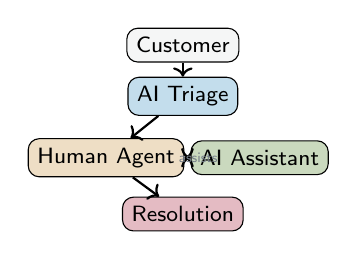
\begin{tikzpicture}[scale=0.65, font=\footnotesize]
                % Flow
                \node[draw, fill=TuebingenBeige, rounded corners] (customer) at (0,3) {Customer};
                \node[draw, fill=TuebingenCyan!30, rounded corners] (triage) at (0,2) {AI Triage};
                \node[draw, fill=TuebingenGold!30, rounded corners] (agent) at (-1.5,0.8) {Human Agent};
                \node[draw, fill=TuebingenGreen!30, rounded corners] (ai) at (1.5,0.8) {AI Assistant};
                \node[draw, fill=TuebingenRot!30, rounded corners] (resolve) at (0,-0.3) {Resolution};
                
                \draw[->, thick] (customer) -- (triage);
                \draw[->, thick] (triage) -- (agent);
                \draw[<->, thick, dashed] (agent) -- (ai);
                \draw[->, thick] (agent) -- (resolve);
                
                % Labels
                \node[font=\tiny, TuebingenGray] at (0.3, 0.8) {assists};
            \end{tikzpicture}
        \end{center}
        
        \vspace{0.3em}
        \textbf{Key Principle:}
        
        \vspace{0.2em}
        {\color{TuebingenGreen} Human in the loop for decisions.}
        
        {\color{TuebingenGreen} AI handles information retrieval + drafting.}
    \end{columns}
\end{frame}

\begin{frame}{Customer Support: Compliance \& Escalation}
    \framesubtitle{Guardrails for customer-facing AI}
    
    \vspace{0.3em}
    \begin{columns}[T]
        \column{0.48\textwidth}
        {\color{TuebingenRot}\textbf{Compliance Constraints:}}
        \begin{itemize}
            \setlength\itemsep{0.4em}
            \item \textbf{Regulated industries:} Financial advice, medical, legal — AI suggests, human approves
            \item \textbf{PII handling:} Don't expose customer data in logs
            \item \textbf{Promises:} AI cannot commit the company
            \item \textbf{Disclaimers:} Required in some contexts
        \end{itemize}
        
        \vspace{0.3em}
        \textbf{Content Policies:}
        \begin{itemize}
            \setlength\itemsep{0.3em}
            \item Tone guidelines
            \item Prohibited topics
            \item Brand voice consistency
        \end{itemize}
        
        \column{0.48\textwidth}
        \textbf{Escalation Rules:}
        \begin{itemize}
            \setlength\itemsep{0.4em}
            \item \textbf{Sentiment:} Angry/frustrated → human
            \item \textbf{Complexity:} Multi-issue → human
            \item \textbf{Risk:} Legal threat → human + legal
            \item \textbf{Value:} High-value customer → human
            \item \textbf{Uncertainty:} Low confidence → human
        \end{itemize}
        
        \vspace{0.3em}
        \begin{theorembox}{Golden Rule}
            When in doubt, escalate. \\
            The cost of over-escalation < cost of wrong answer.
        \end{theorembox}
    \end{columns}
\end{frame}

\begin{frame}{Customer Support: Metrics That Matter}
    \framesubtitle{How to measure success}
    
    \vspace{0.3em}
    \begin{columns}[T]
        \column{0.48\textwidth}
        \textbf{Efficiency Metrics:}
        \begin{itemize}
            \setlength\itemsep{0.4em}
            \item \textbf{Average Handle Time (AHT):}
            \begin{itemize}
                \item Target: 15-30\% reduction
                \item Measure: Time from open to close
            \end{itemize}
            \item \textbf{First Contact Resolution (FCR):}
            \begin{itemize}
                \item Target: 5-10\% improvement
                \item Measure: Resolved without transfer
            \end{itemize}
            \item \textbf{Agent Utilization:}
            \begin{itemize}
                \item More tickets per agent
                \item Less time searching
            \end{itemize}
        \end{itemize}
        
        \column{0.48\textwidth}
        \textbf{Quality Metrics:}
        \begin{itemize}
            \setlength\itemsep{0.4em}
            \item \textbf{CSAT:} Customer satisfaction score
            \item \textbf{QA Score:} Compliance with guidelines
            \item \textbf{Error Rate:} Wrong answers caught
            \item \textbf{Escalation Rate:} Should stay stable
        \end{itemize}
        
        \vspace{0.3em}
        \textbf{AI-Specific Metrics:}
        \begin{itemize}
            \setlength\itemsep{0.3em}
            \item Suggestion acceptance rate
            \item Time saved per suggestion
            \item Retrieval accuracy
        \end{itemize}
    \end{columns}
    
    \vspace{0.5em}
    {\color{TuebingenGray}\textbf{Warning:} Don't optimize AHT at expense of quality. Balance is key.}
\end{frame}

\begin{frame}{Customer Support: Implementation Approach}
    \framesubtitle{Phased rollout for risk control}
    
    \vspace{0.3em}
    \textbf{Phase 1: Shadow Mode (4-6 weeks)}
    \begin{itemize}
        \setlength\itemsep{0.2em}
        \item AI generates suggestions, agents see but don't have to use
        \item Collect feedback: Was this helpful? What was wrong?
        \item Build evaluation dataset from real interactions
    \end{itemize}
    
    \vspace{0.3em}
    \textbf{Phase 2: Assisted Mode (6-8 weeks)}
    \begin{itemize}
        \setlength\itemsep{0.2em}
        \item AI suggestions integrated into workflow
        \item One-click acceptance with edit capability
        \item Measure adoption and quality metrics
    \end{itemize}
    
    \vspace{0.3em}
    \textbf{Phase 3: Enhanced Automation (Optional)}
    \begin{itemize}
        \setlength\itemsep{0.2em}
        \item Auto-draft for simple, low-risk queries
        \item Human review before send (not edit)
        \item Only for high-confidence, low-risk categories
    \end{itemize}
    
    \vspace{0.3em}
    \begin{theorembox}{Success Factor}
        Agent buy-in is critical. Involve agents in design. Position AI as \textbf{tool}, not \textbf{replacement}.
    \end{theorembox}
\end{frame}

% ==============================================================================
% SECTION 3.4: PATTERN 3 — DOCUMENT & WORKFLOW AUTOMATION
% ==============================================================================

\begin{frame}{Pattern 3: Document \& Workflow Automation}
    \framesubtitle{Intelligent document processing at scale}
    
    \vspace{0.3em}
    \begin{columns}[T]
        \column{0.48\textwidth}
        \textbf{What It Is:}
        \begin{itemize}
            \setlength\itemsep{0.3em}
            \item Extract structured data from documents
            \item Route and process automatically
            \item Integrate with business systems
        \end{itemize}
        
        \vspace{0.3em}
        \textbf{Use Cases:}
        \begin{itemize}
            \setlength\itemsep{0.3em}
            \item \textbf{Invoices:} Extract, match, route to AP
            \item \textbf{Claims:} Parse, validate, adjudicate
            \item \textbf{Contracts:} Extract terms, flag risks
            \item \textbf{Procurement:} Process requests
            \item \textbf{Onboarding:} Document verification
        \end{itemize}
        
        \column{0.48\textwidth}
        \begin{center}
            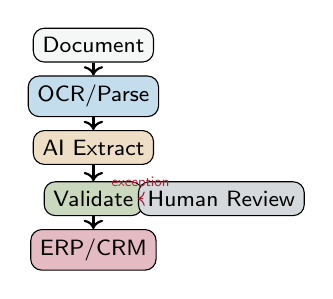
\begin{tikzpicture}[scale=0.65, font=\footnotesize]
                \node[draw, fill=TuebingenBeige, rounded corners] (doc) at (0,2.5) {Document};
                \node[draw, fill=TuebingenCyan!30, rounded corners] (ocr) at (0,1.5) {OCR/Parse};
                \node[draw, fill=TuebingenGold!30, rounded corners] (extract) at (0,0.5) {AI Extract};
                \node[draw, fill=TuebingenGreen!30, rounded corners] (validate) at (0,-0.5) {Validate};
                \node[draw, fill=TuebingenRot!30, rounded corners] (system) at (0,-1.5) {ERP/CRM};
                
                \draw[->, thick] (doc) -- (ocr);
                \draw[->, thick] (ocr) -- (extract);
                \draw[->, thick] (extract) -- (validate);
                \draw[->, thick] (validate) -- (system);
                
                % Exception path
                \node[draw, fill=TuebingenAnthrazit!20, rounded corners] (human) at (2.5,-0.5) {Human Review};
                \draw[->, dashed, TuebingenRot] (validate) -- node[above, font=\tiny] {exception} (human);
            \end{tikzpicture}
        \end{center}
        
        \textbf{Key Principle:}
        
        {\small Always validate before system of record. Exceptions to humans.}
    \end{columns}
\end{frame}

\begin{frame}{Document Automation: Integration is Everything}
    \framesubtitle{The hard part isn't AI — it's connecting systems}
    
    \vspace{0.3em}
    \begin{columns}[T]
        \column{0.48\textwidth}
        \textbf{System Integration Requirements:}
        \begin{itemize}
            \setlength\itemsep{0.4em}
            \item \textbf{Input:} Email, portal, scanner, API
            \item \textbf{Processing:} Workflow engine, queues
            \item \textbf{Output:} ERP, CRM, data warehouse
            \item \textbf{Feedback:} Correction interface
        \end{itemize}
        
        \vspace{0.3em}
        \textbf{Validation Steps:}
        \begin{itemize}
            \setlength\itemsep{0.3em}
            \item Field format checks
            \item Cross-field consistency
            \item Master data lookup (vendor, customer)
            \item Policy rule validation
            \item Duplicate detection
        \end{itemize}
        
        \column{0.48\textwidth}
        \textbf{Why Integration Matters:}
        
        \vspace{0.3em}
        \begin{center}
            \begin{tabular}{@{}lc@{}}
                \toprule
                \textbf{Activity} & \textbf{\% of Effort} \\
                \midrule
                AI/ML model & 20\% \\
                Integration & 40\% \\
                Validation logic & 20\% \\
                Exception handling & 15\% \\
                Monitoring & 5\% \\
                \bottomrule
            \end{tabular}
        \end{center}
        
        \vspace{0.5em}
        {\color{TuebingenGray}\textbf{Reality:} The AI part is often the easy part. Process redesign and integration are where projects succeed or fail.}
    \end{columns}
\end{frame}

\begin{frame}{Document Automation: Failure Modes}
    \framesubtitle{What goes wrong and why}
    
    \vspace{0.3em}
    \begin{columns}[T]
        \column{0.32\textwidth}
        {\color{TuebingenRot}\textbf{OCR Errors:}}
        \begin{itemize}
            \setlength\itemsep{0.2em}
            \item Poor scan quality
            \item Handwritten text
            \item Tables misaligned
            \item Multi-language docs
        \end{itemize}
        
        \vspace{0.2em}
        {\color{TuebingenGreen}\textbf{Fix:}}
        \begin{itemize}
            \setlength\itemsep{0.2em}
            \item Quality gates on input
            \item Confidence thresholds
            \item Human review queue
        \end{itemize}
        
        \column{0.32\textwidth}
        {\color{TuebingenRot}\textbf{Policy Exceptions:}}
        \begin{itemize}
            \setlength\itemsep{0.2em}
            \item Non-standard terms
            \item Unusual amounts
            \item Missing approvals
            \item Edge cases
        \end{itemize}
        
        \vspace{0.2em}
        {\color{TuebingenGreen}\textbf{Fix:}}
        \begin{itemize}
            \setlength\itemsep{0.2em}
            \item Rule-based exception routing
            \item Clear escalation paths
            \item Learn from exceptions
        \end{itemize}
        
        \column{0.32\textwidth}
        {\color{TuebingenRot}\textbf{Adversarial Docs:}}
        \begin{itemize}
            \setlength\itemsep{0.2em}
            \item Fraudulent invoices
            \item Manipulated claims
            \item Hidden terms
        \end{itemize}
        
        \vspace{0.2em}
        {\color{TuebingenGreen}\textbf{Fix:}}
        \begin{itemize}
            \setlength\itemsep{0.2em}
            \item Anomaly detection
            \item Cross-reference checks
            \item Audit sampling
            \item Fraud team integration
        \end{itemize}
    \end{columns}
    
    \vspace{0.5em}
    \begin{theorembox}{Design Principle}
        Assume errors will occur. Design for graceful degradation. \\
        Automation rate of 80\% with 99\% accuracy beats 95\% with 90\% accuracy.
    \end{theorembox}
\end{frame}

\begin{frame}{Document Automation: ROI Model}
    \framesubtitle{Calculating the business case}
    
    \vspace{0.3em}
    \begin{columns}[T]
        \column{0.48\textwidth}
        \textbf{Cost Drivers (Current State):}
        \begin{itemize}
            \setlength\itemsep{0.3em}
            \item Manual data entry time
            \item Error correction rework
            \item Processing delays (float cost)
            \item Compliance failures (penalties)
            \item Missed discounts (late payment)
        \end{itemize}
        
        \vspace{0.3em}
        \textbf{Example: Invoice Processing}
        \begin{itemize}
            \setlength\itemsep{0.2em}
            \item 50,000 invoices/year
            \item \$15 cost per manual invoice
            \item = \$750,000/year baseline
        \end{itemize}
        
        \column{0.48\textwidth}
        \textbf{Automation Benefits:}
        \begin{itemize}
            \setlength\itemsep{0.3em}
            \item 80\% straight-through processing
            \item 70\% cost reduction per invoice
            \item 50\% faster cycle time
            \item 90\% fewer errors
        \end{itemize}
        
        \vspace{0.3em}
        \textbf{ROI Calculation:}
        \begin{itemize}
            \setlength\itemsep{0.2em}
            \item Automated: 40,000 × \$4 = \$160K
            \item Exceptions: 10,000 × \$18 = \$180K
            \item New cost: \$340K
            \item Savings: \$410K/year (55\%)
        \end{itemize}
    \end{columns}
    
    \vspace{0.3em}
    {\color{TuebingenGray}\textbf{Note:} Include implementation cost, maintenance, and ramp-up time in full business case.}
\end{frame}

% ==============================================================================
% SECTION 3.5: PATTERN 4 — SOFTWARE ENGINEERING ACCELERATION
% ==============================================================================

\begin{frame}{Pattern 4: Software Engineering Acceleration}
    \framesubtitle{AI-augmented development}
    
    \vspace{0.3em}
    \begin{columns}[T]
        \column{0.48\textwidth}
        \textbf{What It Is:}
        \begin{itemize}
            \setlength\itemsep{0.3em}
            \item AI integrated into developer workflow
            \item Code completion, generation, search
            \item IDE-native experience
        \end{itemize}
        
        \vspace{0.3em}
        \textbf{Capabilities:}
        \begin{itemize}
            \setlength\itemsep{0.3em}
            \item \textbf{Code completion:} Line/block level
            \item \textbf{Code generation:} From comments/specs
            \item \textbf{Test generation:} Unit tests from code
            \item \textbf{Refactoring:} Suggest improvements
            \item \textbf{Code search:} Natural language queries
            \item \textbf{Documentation:} Generate docs
            \item \textbf{Debugging:} Explain errors
        \end{itemize}
        
        \column{0.48\textwidth}
        \textbf{Tools Landscape:}
        \begin{itemize}
            \setlength\itemsep{0.3em}
            \item \textbf{GitHub Copilot:} Broad adoption
            \item \textbf{Cursor:} IDE with AI-first design
            \item \textbf{Amazon CodeWhisperer:} AWS integration
            \item \textbf{Codeium:} Free tier option
            \item \textbf{Internal:} RAG over your codebase
        \end{itemize}
        
        \vspace{0.3em}
        \textbf{Key Insight:}
        
        \vspace{0.2em}
        {\color{TuebingenGray} These tools are \textbf{RAG systems} specialized for code. Same architecture, different corpus.}
    \end{columns}
\end{frame}

\begin{frame}{Software Engineering: Governance Requirements}
    \framesubtitle{What security and legal need to know}
    
    \vspace{0.3em}
    \begin{columns}[T]
        \column{0.48\textwidth}
        {\color{TuebingenRot}\textbf{Security Risks:}}
        \begin{itemize}
            \setlength\itemsep{0.4em}
            \item \textbf{Secrets exposure:} API keys, credentials in suggestions
            \item \textbf{Code exfiltration:} What goes to the API?
            \item \textbf{Insecure patterns:} AI suggests vulnerable code
            \item \textbf{Dependency risks:} Unknown packages
        \end{itemize}
        
        \vspace{0.3em}
        \textbf{Security Controls:}
        \begin{itemize}
            \setlength\itemsep{0.3em}
            \item Secret scanning in IDE
            \item Allowlist for code sent externally
            \item Security review of AI suggestions
            \item SAST/DAST in CI/CD
        \end{itemize}
        
        \column{0.48\textwidth}
        {\color{TuebingenRot}\textbf{IP/Licensing Risks:}}
        \begin{itemize}
            \setlength\itemsep{0.4em}
            \item \textbf{License contamination:} GPL code in proprietary
            \item \textbf{Copyright claims:} Verbatim reproduction
            \item \textbf{Patent exposure:} Patented algorithms
        \end{itemize}
        
        \vspace{0.3em}
        \textbf{Legal Controls:}
        \begin{itemize}
            \setlength\itemsep{0.3em}
            \item License detection tools
            \item Code similarity scanning
            \item Vendor indemnification review
            \item Clear IP policy for AI-assisted code
        \end{itemize}
    \end{columns}
    
    \vspace{0.3em}
    {\color{TuebingenGray}\textbf{Executive action:} Review vendor agreements. Understand what data flows where. Set clear policy.}
\end{frame}

\begin{frame}{Software Engineering: ROI Measurement}
    \framesubtitle{Quantifying developer productivity gains}
    
    \vspace{0.3em}
    \begin{columns}[T]
        \column{0.48\textwidth}
        \textbf{Productivity Metrics:}
        \begin{itemize}
            \setlength\itemsep{0.4em}
            \item \textbf{Cycle time:} Idea → production
            \item \textbf{Code velocity:} PRs merged/week
            \item \textbf{Time in flow:} Less context switching
            \item \textbf{Onboarding:} Time to first commit
        \end{itemize}
        
        \vspace{0.3em}
        \textbf{Quality Metrics:}
        \begin{itemize}
            \setlength\itemsep{0.3em}
            \item Defect rate (bugs/KLOC)
            \item Test coverage improvement
            \item Code review turnaround
            \item Technical debt reduction
        \end{itemize}
        
        \column{0.48\textwidth}
        \textbf{Published Results:}
        \begin{itemize}
            \setlength\itemsep{0.4em}
            \item GitHub study: 55\% faster task completion
            \item Acceptance rate: 30-40\% of suggestions
            \item Biggest gains: Boilerplate, tests, docs
            \item Smaller gains: Novel/complex logic
        \end{itemize}
        
        \vspace{0.3em}
        \textbf{ROI Calculation:}
        \begin{itemize}
            \setlength\itemsep{0.2em}
            \item 100 developers
            \item \$200K avg fully loaded cost
            \item 10\% productivity gain
            \item = \$2M value/year
            \item Tool cost: \$200K/year
            \item ROI: 10x
        \end{itemize}
    \end{columns}
\end{frame}

\begin{frame}{Software Engineering: Adoption Best Practices}
    \framesubtitle{How to roll out successfully}
    
    \vspace{0.3em}
    \begin{columns}[T]
        \column{0.48\textwidth}
        \textbf{Pilot Design:}
        \begin{itemize}
            \setlength\itemsep{0.4em}
            \item Start with willing early adopters
            \item Mix of senior and junior developers
            \item Clear baseline metrics before
            \item 8-12 week evaluation period
            \item Regular feedback collection
        \end{itemize}
        
        \vspace{0.3em}
        \textbf{Success Factors:}
        \begin{itemize}
            \setlength\itemsep{0.3em}
            \item Developer choice (opt-in)
            \item Good documentation
            \item Champions program
            \item Quick security approval
        \end{itemize}
        
        \column{0.48\textwidth}
        \textbf{Common Pitfalls:}
        \begin{itemize}
            \setlength\itemsep{0.4em}
            \item[$\times$] Mandating tool use
            \item[$\times$] Measuring only code volume
            \item[$\times$] Ignoring security review
            \item[$\times$] No training provided
            \item[$\times$] Expecting magic
        \end{itemize}
        
        \vspace{0.3em}
        \textbf{What to Expect:}
        \begin{itemize}
            \setlength\itemsep{0.3em}
            \item Week 1-2: Learning curve
            \item Week 3-6: Productivity dip possible
            \item Week 7+: Gains materialize
            \item Month 3+: Becomes habit
        \end{itemize}
    \end{columns}
\end{frame}

% ==============================================================================
% SECTION 3.6: PATTERN 5 — DECISION INTELLIGENCE
% ==============================================================================

\begin{frame}{Pattern 5: Decision Intelligence}
    \framesubtitle{AI-augmented business decisions}
    
    \vspace{0.3em}
    \begin{columns}[T]
        \column{0.48\textwidth}
        \textbf{What It Is:}
        \begin{itemize}
            \setlength\itemsep{0.3em}
            \item AI supports human decision-making
            \item Combines prediction + explanation + action
            \item Keeps human accountability
        \end{itemize}
        
        \vspace{0.3em}
        \textbf{Capabilities:}
        \begin{itemize}
            \setlength\itemsep{0.3em}
            \item \textbf{Forecasting:} Demand, revenue, risk
            \item \textbf{Anomaly detection:} Fraud, quality issues
            \item \textbf{Scenario analysis:} What-if modeling
            \item \textbf{Recommendation:} Next best action
            \item \textbf{Explanation:} Why this prediction?
        \end{itemize}
        
        \column{0.48\textwidth}
        {\color{TuebingenRot}\textbf{Critical Warning:}}
        
        \vspace{0.3em}
        \begin{center}
            \fbox{\parbox{0.9\linewidth}{\centering Don't use LLMs as calculators. \\[0.3em] Use tool-based retrieval for numbers.}}
        \end{center}
        
        \vspace{0.3em}
        \textbf{Right Architecture:}
        \begin{itemize}
            \setlength\itemsep{0.3em}
            \item LLM understands question
            \item Tool calls database/model for data
            \item LLM explains results
            \item Numbers come from authoritative source
        \end{itemize}
    \end{columns}
    
    \vspace{0.3em}
    {\color{TuebingenGray}\textbf{Key principle:} AI provides \textbf{information} and \textbf{options}. Humans make \textbf{decisions}.}
\end{frame}

\begin{frame}{Decision Intelligence: Governance \& Accountability}
    \framesubtitle{Who is responsible when AI recommends?}
    
    \vspace{0.3em}
    \begin{columns}[T]
        \column{0.48\textwidth}
        \textbf{Explainability Requirements:}
        \begin{itemize}
            \setlength\itemsep{0.4em}
            \item \textbf{What:} What is the recommendation?
            \item \textbf{Why:} What factors drove it?
            \item \textbf{Confidence:} How certain?
            \item \textbf{Alternatives:} What else considered?
            \item \textbf{Data:} What information used?
        \end{itemize}
        
        \vspace{0.3em}
        \textbf{Regulatory Context:}
        \begin{itemize}
            \setlength\itemsep{0.3em}
            \item EU AI Act: High-risk categories
            \item Fair lending: Adverse action reasons
            \item Insurance: Actuarial justification
            \item HR: Non-discrimination proof
        \end{itemize}
        
        \column{0.48\textwidth}
        \textbf{Accountability Model:}
        
        \vspace{0.3em}
        \begin{center}
            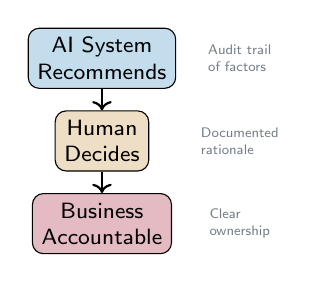
\begin{tikzpicture}[scale=0.7, font=\footnotesize]
                \node[draw, fill=TuebingenCyan!30, rounded corners, align=center] (ai) at (0,2) {AI System\\Recommends};
                \node[draw, fill=TuebingenGold!30, rounded corners, align=center] (human) at (0,0.5) {Human\\Decides};
                \node[draw, fill=TuebingenRot!30, rounded corners, align=center] (outcome) at (0,-1) {Business\\Accountable};
                
                \draw[->, thick] (ai) -- (human);
                \draw[->, thick] (human) -- (outcome);
                
                \node[font=\tiny, TuebingenGray, align=left] at (2.5, 2) {Audit trail\\of factors};
                \node[font=\tiny, TuebingenGray, align=left] at (2.5, 0.5) {Documented\\rationale};
                \node[font=\tiny, TuebingenGray, align=left] at (2.5, -1) {Clear\\ownership};
            \end{tikzpicture}
        \end{center}
        
        \vspace{0.3em}
        {\color{TuebingenGray} AI is a tool. Accountability stays with humans.}
    \end{columns}
\end{frame}

\begin{frame}{Decision Intelligence: Use Case Examples}
    \framesubtitle{Concrete applications}
    
    \vspace{0.3em}
    \begin{columns}[T]
        \column{0.48\textwidth}
        \textbf{Demand Forecasting:}
        \begin{itemize}
            \setlength\itemsep{0.3em}
            \item Input: Historical sales, seasonality, events
            \item Model: Time series + external factors
            \item Output: Forecast + confidence interval
            \item Action: Inventory planning
            \item Governance: Track forecast accuracy
        \end{itemize}
        
        \vspace{0.3em}
        \textbf{Credit Risk:}
        \begin{itemize}
            \setlength\itemsep{0.3em}
            \item Input: Application + bureau data
            \item Model: Scoring model (explainable)
            \item Output: Risk score + factors
            \item Action: Approve/decline/review
            \item Governance: Fair lending compliance
        \end{itemize}
        
        \column{0.48\textwidth}
        \textbf{Fraud Detection:}
        \begin{itemize}
            \setlength\itemsep{0.3em}
            \item Input: Transaction stream
            \item Model: Anomaly detection
            \item Output: Alert + risk score
            \item Action: Review queue priority
            \item Governance: False positive tracking
        \end{itemize}
        
        \vspace{0.3em}
        \textbf{Pricing Optimization:}
        \begin{itemize}
            \setlength\itemsep{0.3em}
            \item Input: Market, inventory, demand
            \item Model: Elasticity + competition
            \item Output: Price recommendation
            \item Action: Human approval required
            \item Governance: Margin guardrails
        \end{itemize}
    \end{columns}
\end{frame}

% ==============================================================================
% SECTION 3.7: PATTERN 6 — OPERATIONS & QUALITY
% ==============================================================================

\begin{frame}{Pattern 6: Operations \& Quality}
    \framesubtitle{AI in physical operations}
    
    \vspace{0.3em}
    \begin{columns}[T]
        \column{0.48\textwidth}
        \textbf{Use Cases:}
        \begin{itemize}
            \setlength\itemsep{0.4em}
            \item \textbf{Predictive maintenance:}
            \begin{itemize}
                \item Sensor data → failure prediction
                \item Schedule maintenance proactively
            \end{itemize}
            \item \textbf{Quality inspection:}
            \begin{itemize}
                \item Visual inspection (CNNs)
                \item Defect detection at speed
            \end{itemize}
            \item \textbf{Supply chain:}
            \begin{itemize}
                \item Demand forecasting
                \item Logistics optimization
            \end{itemize}
        \end{itemize}
        
        \column{0.48\textwidth}
        \textbf{When to Use Deep Learning:}
        \begin{itemize}
            \setlength\itemsep{0.4em}
            \item[$\checkmark$] Unstructured data (images, signals)
            \item[$\checkmark$] Complex patterns
            \item[$\checkmark$] Large training data available
            \item[$\checkmark$] Clear ground truth
        \end{itemize}
        
        \vspace{0.3em}
        \textbf{When Classical Methods Win:}
        \begin{itemize}
            \setlength\itemsep{0.4em}
            \item[$\checkmark$] Structured tabular data
            \item[$\checkmark$] Need explainability
            \item[$\checkmark$] Limited training data
            \item[$\checkmark$] Simpler pattern recognition
        \end{itemize}
    \end{columns}
    
    \vspace{0.3em}
    {\color{TuebingenGray}\textbf{Key insight:} Not every operations problem needs deep learning. Match method to problem.}
\end{frame}

\begin{frame}{Operations: Implementation Considerations}
    \framesubtitle{Unique challenges in physical systems}
    
    \vspace{0.3em}
    \begin{columns}[T]
        \column{0.48\textwidth}
        \textbf{Data Challenges:}
        \begin{itemize}
            \setlength\itemsep{0.4em}
            \item \textbf{Sensor quality:} Noise, drift, gaps
            \item \textbf{Labeling:} Few failures to learn from
            \item \textbf{Edge deployment:} Limited compute
            \item \textbf{Latency:} Real-time requirements
        \end{itemize}
        
        \vspace{0.3em}
        \textbf{Integration Requirements:}
        \begin{itemize}
            \setlength\itemsep{0.3em}
            \item SCADA/PLC connectivity
            \item MES/ERP integration
            \item Alert routing to operators
            \item Maintenance scheduling
        \end{itemize}
        
        \column{0.48\textwidth}
        \textbf{Success Factors:}
        \begin{itemize}
            \setlength\itemsep{0.4em}
            \item \textbf{Domain expertise:} Work with operators
            \item \textbf{Baseline:} Measure current performance
            \item \textbf{Pilot scope:} One line, one failure mode
            \item \textbf{Trust building:} Gradual rollout
        \end{itemize}
        
        \vspace{0.3em}
        \textbf{ROI Metrics:}
        \begin{itemize}
            \setlength\itemsep{0.3em}
            \item Unplanned downtime reduction
            \item Defect escape rate
            \item Maintenance cost savings
            \item Throughput improvement
        \end{itemize}
    \end{columns}
    
    \vspace{0.3em}
    {\color{TuebingenGray}\textbf{Reality check:} Operations AI often has longest implementation time but highest sustained ROI.}
\end{frame}

% ==============================================================================
% SECTION 3.8: WHY PILOTS FAIL & WHAT SUCCESS LOOKS LIKE
% ==============================================================================

\begin{frame}{Why AI Pilots Fail}
    \framesubtitle{Lessons from the field}
    
    \vspace{0.3em}
    \begin{columns}[T]
        \column{0.48\textwidth}
        {\color{TuebingenRot}\textbf{Failure Mode 1: No Process Owner}}
        \begin{itemize}
            \setlength\itemsep{0.2em}
            \item IT builds it, business doesn't adopt
            \item No one accountable for outcomes
            \item Dies when champion leaves
        \end{itemize}
        
        \vspace{0.3em}
        {\color{TuebingenRot}\textbf{Failure Mode 2: Poor Data}}
        \begin{itemize}
            \setlength\itemsep{0.2em}
            \item Garbage in, garbage out
            \item Data quality discovered too late
            \item No budget for data remediation
        \end{itemize}
        
        \vspace{0.3em}
        {\color{TuebingenRot}\textbf{Failure Mode 3: No Integration}}
        \begin{itemize}
            \setlength\itemsep{0.2em}
            \item Standalone demo, not in workflow
            \item Extra steps vs. current process
            \item No system of record connection
        \end{itemize}
        
        \column{0.48\textwidth}
        {\color{TuebingenRot}\textbf{Failure Mode 4: No Evaluation}}
        \begin{itemize}
            \setlength\itemsep{0.2em}
            \item Ship and hope
            \item No baseline metrics
            \item Can't prove value (or problems)
        \end{itemize}
        
        \vspace{0.3em}
        {\color{TuebingenRot}\textbf{Failure Mode 5: No Change Management}}
        \begin{itemize}
            \setlength\itemsep{0.2em}
            \item Users not trained
            \item Resistance not addressed
            \item Process not redesigned
        \end{itemize}
        
        \vspace{0.3em}
        {\color{TuebingenRot}\textbf{Failure Mode 6: Wrong Problem}}
        \begin{itemize}
            \setlength\itemsep{0.2em}
            \item Tech looking for problem
            \item Low value use case
            \item Unstable process to automate
        \end{itemize}
    \end{columns}
\end{frame}

\begin{frame}{What Success Looks Like}
    \framesubtitle{Characteristics of AI initiatives that scale}
    
    \vspace{0.3em}
    \begin{columns}[T]
        \column{0.48\textwidth}
        \textbf{Process Characteristics:}
        \begin{itemize}
            \setlength\itemsep{0.4em}
            \item[$\checkmark$] \textbf{Measurable:} Clear KPIs before/after
            \item[$\checkmark$] \textbf{Stable:} Process doesn't change weekly
            \item[$\checkmark$] \textbf{High volume:} Worth automating
            \item[$\checkmark$] \textbf{Clear handoffs:} Defined inputs/outputs
            \item[$\checkmark$] \textbf{Data available:} Ground truth exists
        \end{itemize}
        
        \vspace{0.3em}
        \textbf{Organizational Readiness:}
        \begin{itemize}
            \setlength\itemsep{0.3em}
            \item[$\checkmark$] Executive sponsor committed
            \item[$\checkmark$] Process owner identified
            \item[$\checkmark$] Users engaged in design
            \item[$\checkmark$] IT/Security aligned
        \end{itemize}
        
        \column{0.48\textwidth}
        \textbf{Success Indicators:}
        \begin{itemize}
            \setlength\itemsep{0.4em}
            \item Users ask for expansion
            \item Metrics improve measurably
            \item Process owner wants more budget
            \item Other teams request similar
            \item Feedback loop generates improvements
        \end{itemize}
        
        \vspace{0.3em}
        \begin{theorembox}{Success Formula}
            \textbf{Clear problem} + \textbf{Good data} + \\ \textbf{Process owner} + \textbf{Measured outcomes} \\ + \textbf{Change management} = Scale
        \end{theorembox}
    \end{columns}
\end{frame}

\begin{frame}{Act III: Summary}
    \framesubtitle{Business patterns you can fund and govern}
    
    \vspace{0.3em}
    \begin{columns}[T]
        \column{0.48\textwidth}
        \textbf{Six Proven Patterns:}
        \begin{enumerate}
            \setlength\itemsep{0.3em}
            \item \textbf{Knowledge Assistant:} Quick wins, clear ROI
            \item \textbf{Customer Support:} High visibility, compliance needs
            \item \textbf{Document Automation:} Integration-heavy, high savings
            \item \textbf{Software Engineering:} Developer productivity
            \item \textbf{Decision Intelligence:} Explainability critical
            \item \textbf{Operations:} Longest timeline, sustained ROI
        \end{enumerate}
        
        \column{0.48\textwidth}
        \textbf{Universal Success Factors:}
        \begin{itemize}
            \setlength\itemsep{0.4em}
            \item Process owner with accountability
            \item Clear metrics before you start
            \item Integration into real workflow
            \item Evaluation and feedback loops
            \item Change management investment
        \end{itemize}
        
        \vspace{0.3em}
        {\color{TuebingenGray}\textbf{Pattern selection:} Match to your organization's strengths, data assets, and risk tolerance.}
    \end{columns}
    
    \vspace{0.5em}
    \begin{theorembox}{Next: Act IV}
        How to deliver these patterns: lifecycle, governance, economics, and vendor strategy.
    \end{theorembox}
\end{frame}

% Act IV — Operating Model, Governance, Benchmarking
\section{Operating Model, Governance, Benchmarking}
% ...existing content to be filled in...

% Act V — Transition to Tailored Needs Analysis
\section{Transition to Tailored Needs Analysis}
% ...existing content to be filled in...


% --- 5. DARK SUMMARY SLIDE ---
{ 
% Local color override for Dark Mode
\setbeamercolor{background canvas}{bg=TuebingenAnthrazit}
\setbeamercolor{normal text}{fg=white}
\setbeamercolor{itemize item}{fg=white}
\setbeamercolor{structure}{fg=white}

\begin{frame}[plain]
    \begin{columns}
        \column{0.6\textwidth}
            {\color{white}\textbf{\Large Summary}}
            \vspace{1em}
            \begin{itemize}
                \setlength\itemsep{1em}
                \item {\color{white}Summary point 1}
                \item {\color{white}Summary point 2}
                \item {\color{white}Summary point 3}
                \item {\color{white}Summary point 4}
            \end{itemize}

        \column{0.4\textwidth}
            \centering
            \vspace{1em}
            {\color{white}Thank you!}
    \end{columns}
    
    % Manual Footer for Dark Slide
    \vspace{2cm}
    \begin{tikzpicture}[remember picture, overlay]
         \node[anchor=south west, white] at ([xshift=0.5cm, yshift=0.2cm]current page.south west) {\tiny Course Name \#\lecturenumber \ -- \ \the\year \ \insertauthor, \license \ -- \ \shortdate};
         \node[anchor=south east, white] at ([xshift=-0.5cm, yshift=0.2cm]current page.south east) {\tiny \insertframenumber};
    \end{tikzpicture}
\end{frame}
}

\end{document}